\documentclass[12pt]{ociamthesis}  % default square logo 
%\documentclass[12pt,beltcrest]{ociamthesis} % use old belt crest logo
%\documentclass[12pt,shieldcrest]{ociamthesis} % use older shield crest logo

%load any additional packages
\usepackage{amssymb}

%\input{packages}
\include{import}
\usepackage[backend=bibtex]{biblatex}
\addbibresource{refs.bib}

\usepackage{times}
\usepackage{epsfig}
\usepackage{graphicx}
\usepackage{amsmath}
\usepackage{amssymb}
\usepackage{dsfont}
\usepackage{enumitem}
\usepackage{multicol}
\usepackage{multirow}
\usepackage{amsbsy}
\usepackage{array, caption, tabularx, makecell, booktabs}%
\usepackage{animate}
%\usepackage{floatrow}
\usepackage{etoolbox}
\usepackage{float}
\usepackage{pdfpages}
%\usepackage[titletoc]{appendix}
\usepackage{appendix}
\DeclareMathOperator{\E}{\mathbb{E}}
\DeclareMathOperator{\R}{\mathbb{R}}

\def\figref#1{Fig.~\ref{#1}}
\def\secref#1{\S\ref{#1}}
\def\tabref#1{Table~\ref{#1}}
\def\eqnref#1{Eq.~\ref{#1}}
\def\etal{et al.}
\def\eg{For example}

\usepackage{subcaption}
\captionsetup{compatibility=false}

\graphicspath{ {figures/chapter_1/syntheticExp/} {figures/chapter_1/images/} {figures/chapter_3/}  }

%input macros (i.e. write your own macros file called mymacros.tex 
%and uncomment the next line)
%\include{mymacros}

\title{Deep Generative Models: Analysis through algorithms and applications to Computer Graphics} 

% \title{Codimension-Two\\[1ex]     %your thesis title,
%         Free Boundary Problems}   %note \\[1ex] is a line break in the title

\author{Arnab Ghosh}             %your name
\college{St Cross College}  %your college

%\renewcommand{\submittedtext}{change the default text here if needed}
\degree{Doctor of Philosophy}     %the degree
\degreedate{Trinity 2021}         %the degree date

%end the preamble and start the document
\begin{document}

%this baselineskip gives sufficient line spacing for an examiner to easily
%markup the thesis with comments
\baselineskip=18pt plus1pt

%set the number of sectioning levels that get number and appear in the contents
\setcounter{secnumdepth}{3}
\setcounter{tocdepth}{3}


\maketitle                  % create a title page from the preamble info
\begin{originality}

This thesis is submitted to the Department of Engineering Science, University of
Oxford, in fulfilment of the requirements for the degree of Doctor of Philosophy.
This thesis is entirely my own work, and except where otherwise stated, describes
my own research.

Arnab Ghosh, St Cross College

\end{originality}        % include a dedication.tex file
\begin{acknowledgements}

I would like to thank my supervisor, Prof.~Phil Torr, for having faith in me and providing the opportunity to pursue a PhD.
His infectious energy and creativity have been pivotal in making this thesis possible.

I have also had the pleasure of working closely with many collaborators during my PhD. 
My mentors in my initial projects -- Michael, Ondra, Stuart and Sadeep -- have played a significant role in my development as a researcher.
I have also enjoyed subsequent collaborations with Kyle, Qizhu, M{\aa}ns, Fredrik, Li, Rodrigo and Carl.
Further thanks go to the computer vision teams in DeepMind and Google (particularly Abhanshu, Matt and Sammy) for hosting me. %during two \FIX{unforgettable} summers.
Bernardino and Stuart have also taken the time to provide detailed and thoughtful feedback on drafts of my papers on numerous occasions.

I have been fortunate to be part of the computer vision community in Oxford.
There are too many past and present members in TVG to name here, along with many others from VGG, OVAL and AVL from whom I have learned things from whilst sharing an ``office''.
One of the best perks of studying at Oxford has been the impressive array of seminar speakers who have given talks here and then been available for further discussions afterwards.
%Another advantage of the large research community at Oxford has been the impressive array of seminar speakers who have visited and given talks here.
I am also grateful to my transfer report examiners, Professors Pawan Kumar and Paul Newman, and also Prof.~Andrew Zissermann whom I collaborated with.
My thesis examiners, Professors Andrea Vedaldi and Iasonas Kokkinos, also provided insightful comments on the manuscript and the viva itself turned out to be a stimulating discussion.

\iffalse
Furthermore, it has been a priviledge to regularly have 

 have a steady stream of invited seminar speakers, and 

, -- there are too many past and present members in TVG to name here, along with many other

-- multiple reserach groups
-- top speakers
	-- In both cases, I have learned cool stuff from them.
	-- had good audience questions
-- transfer report, AZ
	
I have been fortunate to be part of the computer vision community in Oxford, with its impressive array of invited seminar speakers, and filled with many great minds from whom I have learned a lot from.
There are too many past and present members in TVG to name here, along with many others from VGG, OVAL and AVL.
I am also grateful to my transfer report examiners, Professors Pawan Kumar and Paul Newman, and also Prof. Andrew Zisserman whom I collaborated with and learned a lot from.
\fi

I have thoroughly enjoyed my time here in Oxford, both inside and outside of the lab, thanks to Sven, Aravindh, Namhoon, Jessamy, Qizhu, Li, Arnab, Harkirat, Daniela, Oscar, Piotr, Vivek and the badminton clubs of Linacre and Jesus College.

Maddy, and then later Cassandra, have also been helpful regarding all administrative matters.
And thanks to Jerry, as well as the ARC team, for managing the group's computing resources.

I am grateful to my family for their continual support during my PhD. In particular, I am thankful to Didi for proof-reading yet another thesis and spoiling me on every vacation.

Finally, I am grateful to have been funded by the Clarendon Scholarship.

\iffalse
I have also had the pleasure of working closely with 

I have been fortunate to be part of the Torr Vision Group, filled with many great minds from whom I have learned a lot from.
Furthermore


I have been fortunate to be part of the computer vision community in Oxford 

I have been fortunate to be part of the Torr Vision Group, filled with many great minds from whom I have learned a lot from.
	
I would like to thank my supervisor, Prof. Phil Torr, for having faith in me and providing the opportunity to pursue a PhD.
Phil's infectious passion, energy and creativity 
% and willingness to support my work even when he did not agree with it
has been pivotal in making this thesis possible.

I have been fortunate to be part of the Torr Vision Group 

for having faith in me, giving me a chance, supporting me even when I went against his wishes,	
	
Phil passion and creativity

Transfer report examiners, Professors Pawan Kumar and Paul Newman.
Also fortunate to work with Andrew Zisserman.

Collaborators: early on: Michael, Ondra, Stuart, Sadeep
More collaborators: Kyle, Mans, Fredrick, Qizhu, Carl

AZ, Carl at DeepMind, Abhanshu, Sammy and Matt at Google

Lab at Oxford -- TVG, Oval and VGG enriching experience.
Great speakers at seminars

Social: Namhoon, Qizhu, Li, Arnab, Harkirat, Daniela
Sven, Jessamy

Bernardino and Stuart for feedback on my papers.

Clarendon Scholarship, for supporting my DPhil studies.
Maddy, Cassandra and Lincare College for all adminstrative queries

Family for support. In particular, Didi, for proof-reading yet another thesis and spoiling me on vacations.
\fi

\end{acknowledgements}   % include an acknowledgements.tex file
\begin{abstract}

Although humans can effortlessly recognise a scene in its totality, it is an extremely challenging problem for computers which is why scene understanding remains one of the fundamental problems in computer vision.
%
% Humans can effortlessly recognise everything they see in a scene. \TODO{need a bit more here}
% However, scene understanding is extremely challenging for computers, and one of the fundamental problems of computer vision.
This thesis concentrates on pixel-level scene understanding tasks such as semantic- and instance-segmentation, which have applications in diverse fields such as autonomous vehicles, medical diagnosis and assistive technologies for the partially sighted among others.
% Semantic segmentation aims to label each pixel in an image with an object class label, instance segmentation extends this by also assigning a unique instance identifier to each 

Firstly, this thesis addresses the task of semantic segmentation by integrating mean-field inference of a Conditional Random Field (CRF) with higher order potentials directly into a deep neural network.
This approach enables joint, end-to-end training of both the parameters of the CRF and the underlying CNN, and achieved state-of-the-art results on public leaderboards at the time of publication.

This method is then extended to the task of instance segmentation.
In contrast to previous work, the proposed formulation jointly processes all instances in the image.
As such, one pixel can only be assigned to one instance and the network must thus learn to reason about occlusions between instances.
Moreover, unlike previous work, this approach can naturally segment ``stuff'' classes.
This method also achieved state-of-the-art results at the time of publication.

Realising the fact that pixel-level training data for segmentation is time-consuming and thus expensive to obtain, this thesis then proposes a method of training semantic- and instance-segmentation models with weaker supervision.
In particular, annotations in the form of bounding-boxes and image-level tags are considered, which are shown to significantly reduce annotation time with a relatively small impact on the final performance compared to a fully-supervised baseline.

Finally, this thesis studies the adversarial robustness of popular semantic segmentation architectures.
This topic is motivated by the fact that during the course of this thesis, segmentation systems have become accurate enough to use in real-world applications, and thus the security of models deployed in production is critical.
The effect of various architectural components on adversarial robustness are thoroughly evaluated, and mean-field inference of CRFs, multiscale processing (and more generally, input transformation) are shown to naturally implement concurrently proposed adversarial defences.
% This study will aid future efforts developing models that are robust to adversarial attacks without compromising on accuracy.

\iffalse
	The observations from this study provide insight into how we can train models that are both accurate and robust to adversarial attacks.
	
	 motivated by the fact that semantic segmentation systems have, during the course of this thesis, becoming accurate eno
	
	considering that during the course of this thesis, se
	
	
	This thesis first addresses the problem of semantic segmentation by c
	
	This thesis first addresses the problem of semantic segmentation by proposing a Conditional Random Field (CRF) with higher order potentials.
	The iterative mean-field inference algorithm for CRFs is unrolled and formulated as a recurrent neural network, enabling end-to-end training of both the parameters of the CRF and underlying CNN jointly.
	
	Mean-field inference of this CRF is unrolled
	 
	Humans can effortlessly recognise everything they see in a scene.
	Examples are types of objects present, number of them, specific location etc
	However, scene understanding is extremely challenging for computers, and one of the fundamental problems of computer vision
	This thesis concentrates on pixel-level scene understanding tasks such as semantic segmentation -- -- and instance segmentation -- --
	Solving these tasks would enable numerous tasks such as autonomous vehicles, medical diagnosis, ar/vr, glasses for partially sighted.
	
	First address the problem of semantic segmentation
	Model structure of the problem with Conditional Random Fields with Higher Order potentials, and show how mean-field inference of this CRF can be unrolled and interpreted as a neural network.
	Gives us the benefits of both CRFs (prior) and CNN (learn from data).
	Top performance on Pascal VOC benchmark at the time.
	
	Extend this approach to the task of instance segmentation. In contrast to previous work, our formulation jointly processes all instances in the image. As such, one pixel can only be assigned to one instance, and the network must thus learn to reason about occlusions between instances. Furthermore, no problem with dealing with ``stuff'' classes unlike previous work.
	Leading performance on Cityscapes benchmark.
	
	Realising the cost of obtaining annotation, then propose a weakly supervised method of training the semantic- and instance-segmentation networks proposed in this thesis.
	Only bounding-box and image-level tags as annotation, use approach based on the self-training paradigm, still able to achieve up to 95\% of fully-supervised performance in some cases.
	
	Finally, considering that segmentation systems have during the course of the thesis become accurate enough to use in practical applications such as autonomous cars, we consider their security.
	Specifically, we study the adversarial robustness of various segmentation architectures.
	Find that mean-field inference causes gradient masking, and input transformations do X.
	Will help future efforts to understand and develop defences to adversarial examples that are robust whilst not compromising predictive accuracy.
\fi

\end{abstract}          % include the abstract

\begin{romanpages}          % start roman page numbering
\tableofcontents            % generate and include a table of contents
\listoffigures              % generate and include a list of figures
\end{romanpages}            % end roman page numbering

%now include the files of latex for each of the chapters etc
%\include{chapter1}
%\include{chapter2}
%\include{conclusions}

\chapter{Introduction}

\section{Generative Models}
\label{sec:intro_generative_models}

\begin{quote}
	What I cannot create, I do not understand - Richard Feynman
\end{quote}

\begin{figure}[ht!]
	\centering
	\begin{tabular}{cc}
		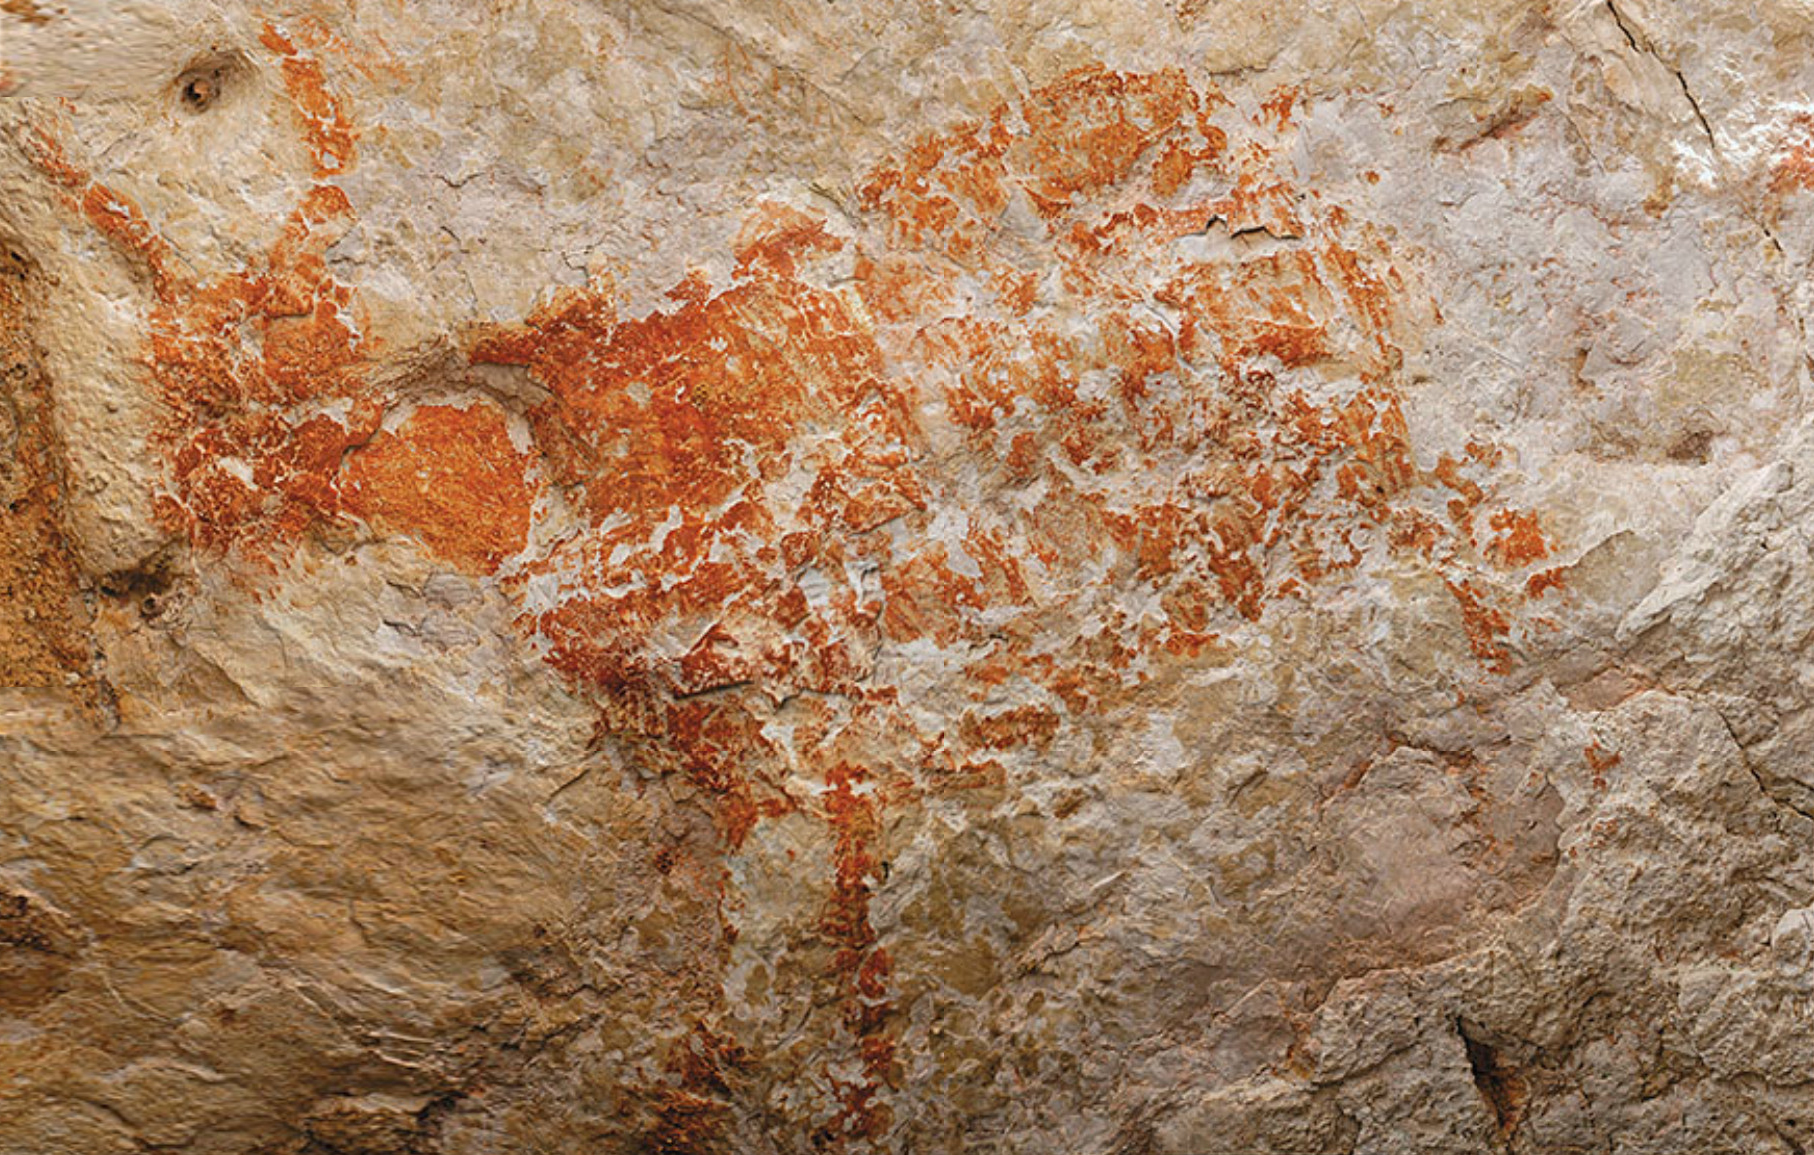
\includegraphics[width=0.49\linewidth]{figures/intro/cave_painting_of_bull.jpeg} &
		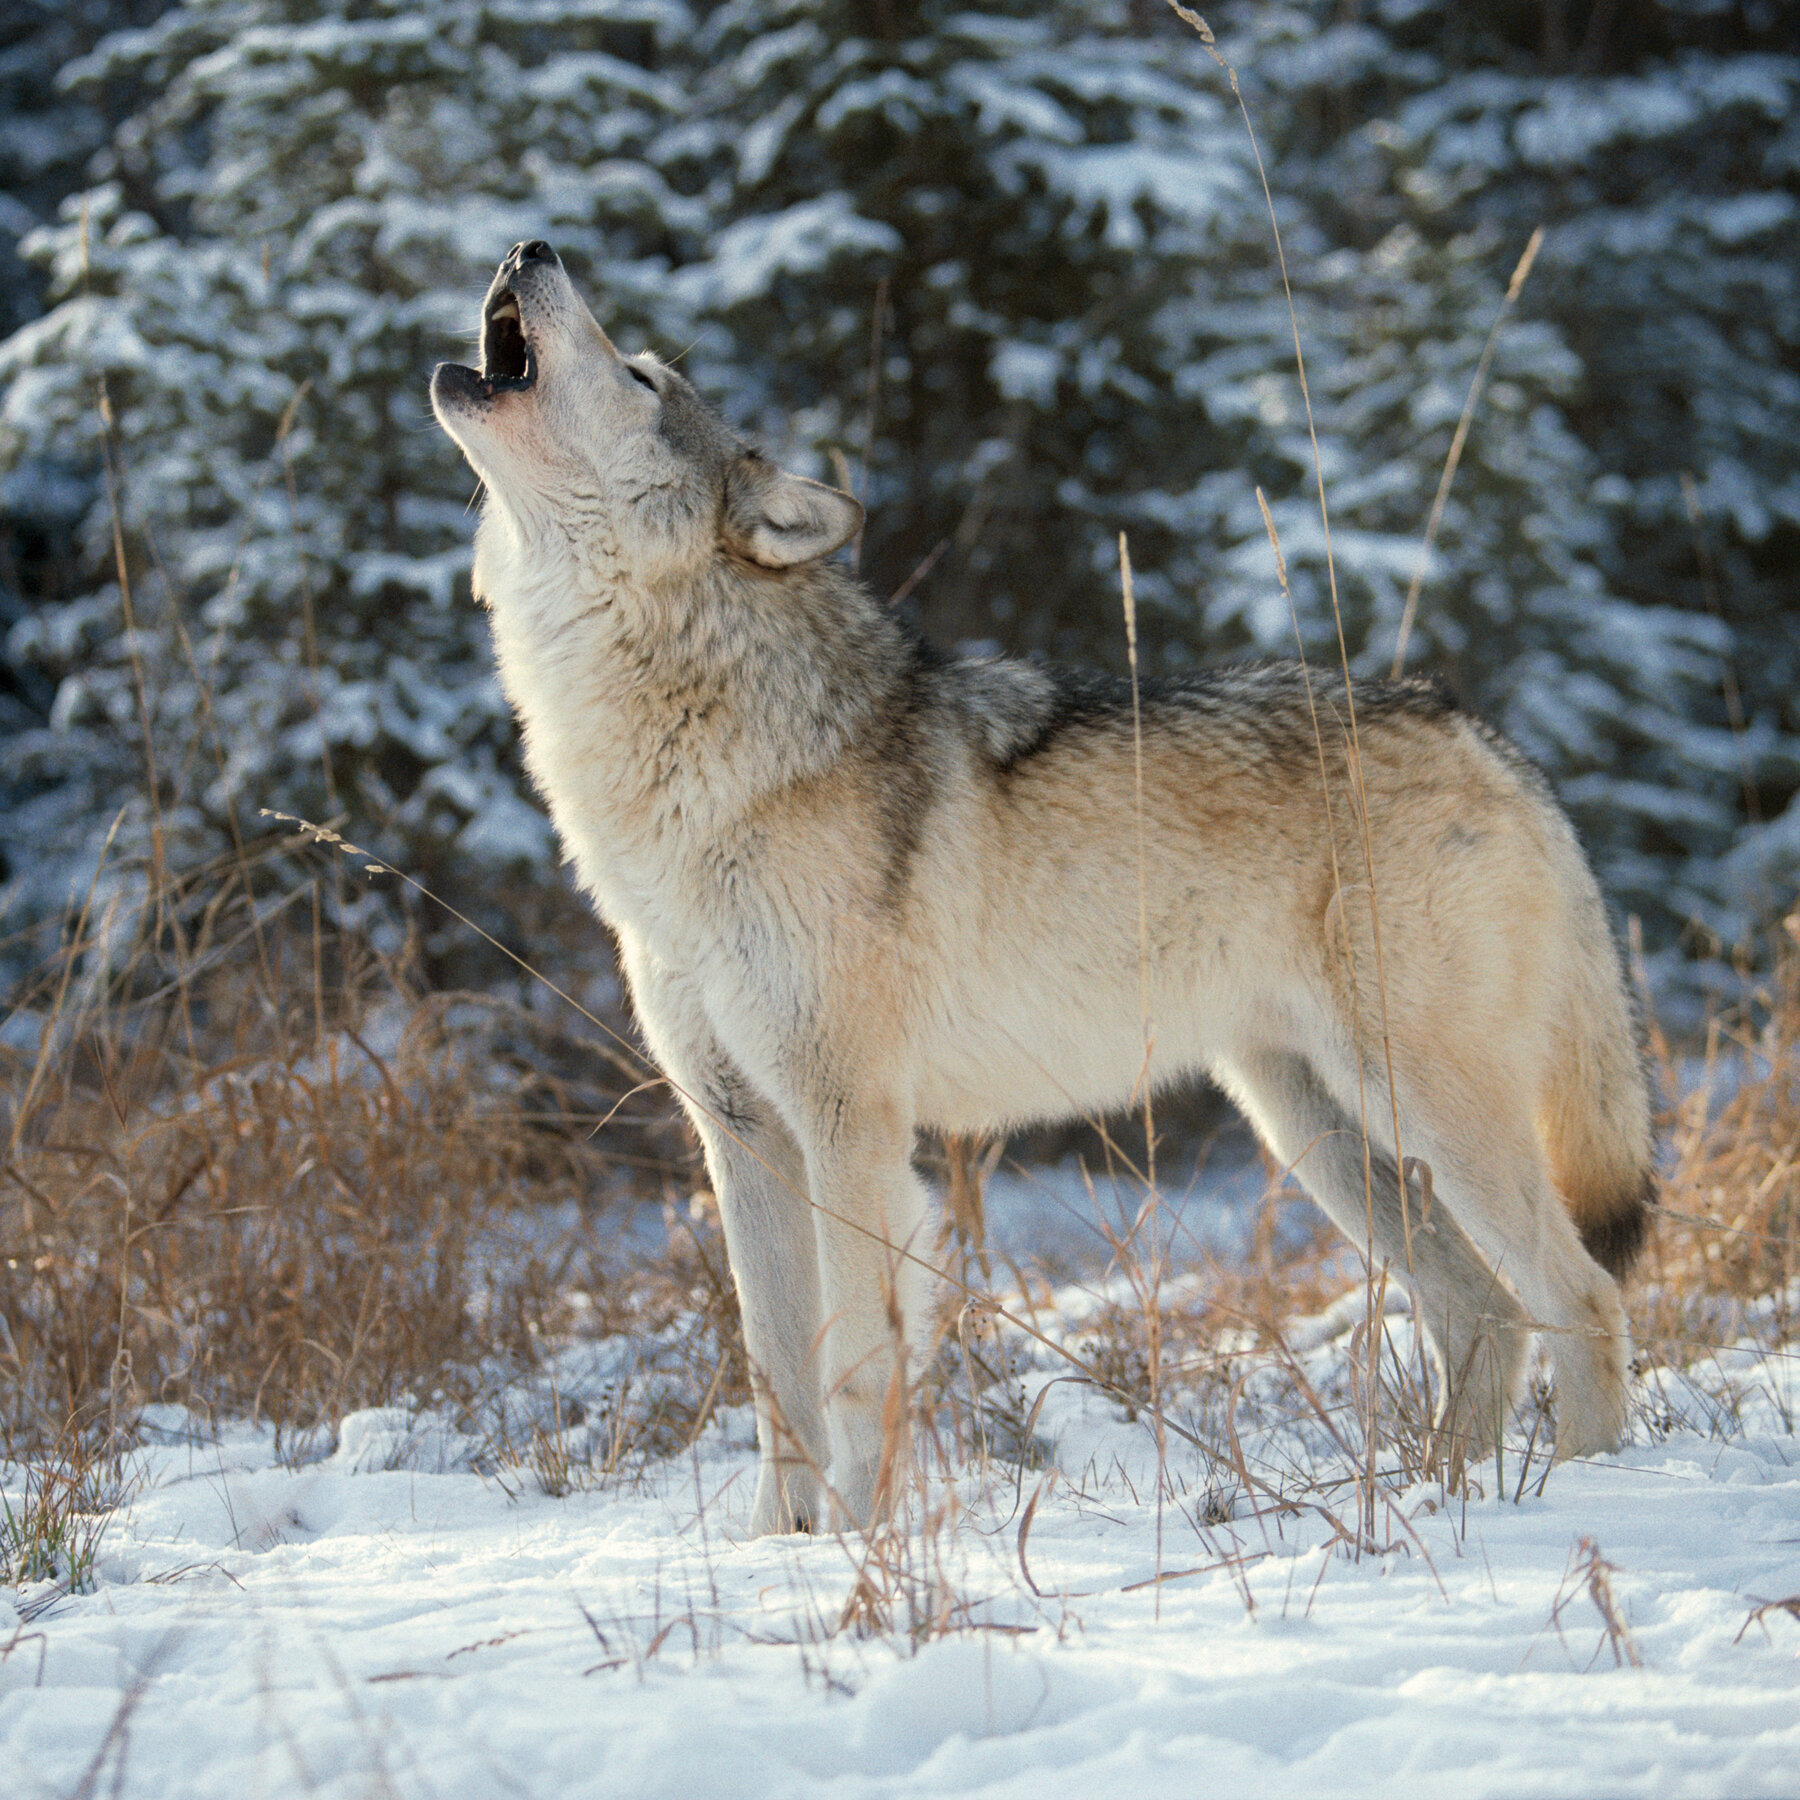
\includegraphics[width=0.31\linewidth]{figures/intro/wolf_nyt.jpeg}
		\\
	%(a) One of the oldest known figurative paintings, a depiction of an unknown bovine, was discovered in the Lubang Jeriji Saléh cave and dated to be more than 40,000 (perhaps as old as 52,000) years old. & (b) Recent photograph of a wolf from New York Times
	\end{tabular}	
	\caption[Efficacy of visual communication]{
		We are able to recognize the bovine creature almost as succinctly as we understand the wolf. However if we're magically transported to the past when this was being painted we wouldn't understand any of the language being spoken.
		}
	\label{fig:cave_painting}
\end{figure}

Visual communication had been the primary method of communication since time immemorial. If we go back to some of the earliest known cave paintings more than 10,000 years ago, we would still recognize what they were trying to communicate. As seen in Figure \ref{fig:cave_painting}. Language evolved in humans as a form of communication since the tools to communicate visually were non ubiquitous. If a wolf was nearby and someone started drawing it would already be too late to save anyone.

The tools at the time didn't enable us to draw a wolf fast enough to stop us from being eaten. Thus humans invented language as a means to communicate. If we suddenly invent a time machine and go back thousands of years to the caves with the earliest cave paintings, we would still understand the bull and the impending danger to the human settlement. However if we try to communicate in either English or any other modern language with the prehistoric cave dwellers neither of us would be able to communicate with the other. However, if we showed them a TikTok video of another human, even the prehistoric cave dwellers would most likely be able to identify with the emotions shown in the video. 

\paragraph{Language  as  a bottleneck}
Language along with the immense benefits which depends upon a shared context has as its achilles heel the same thing which makes it most powerful: shared context. When we talk about our Italian holiday, it can mean so many different things to different people. Some would focus on the feel of the air, others on the mediterranean weather. Others on piazzas. Some would envision the passion for the Ferrari F1 team while others might imagine the obvious taste of the delicious pizzas. All of the above is compressed in a single phrase titled "Italian holiday".

\paragraph{Why is visual communication important}

\begin{itemize}
	\item \textbf{Expressing Emotions:} are hard to express via text on the internet
	
	\item \textbf{Saves time:}
	
	\item \textbf{Promotes consistency:}
	
	\item \textbf{Provides Clarity:}
	
	\item \textbf{Increases retention:}
	
	\item \textbf{Universally understood:}
	
	\item \textbf{More impactful:}
	
\end{itemize}


\paragraph{Current state of the art in Visual Communication for mere mortals}

GIFs are the go to medium for expressing our emotions at the moment. Platforms such as Instagram, snapchat and Tiktok have changed how we communicate visually. Tiktok allows us to make videos which would have taken hours of work on Adobe Premier Pro. Instagram and the modern smartphone cameras have rendered the bulky DSLRs obsolete. We now have Google Lens which can identify anything you don’t know in a matter of seconds. 

\paragraph{Future of visual communication}

Interesting products coming to the forefront. Interactive product design in Virtual reality via the oculuses and the holo lenses of the world. 
Just like when you search “How to” on google, and it starts suggesting “how to give a swashbuckling speech on Toastmasters”. Products from Adobe are coming up which starts autocompleting your sketches and also photo-realisitically renders it.
So with a few strokes of your stylus you can design \& customise  your own luxury sports car or your new set of fancy boots.
 In the future when you can 3D print items, you can quickly design your stuff assisted with Ai and just 3D print it at home. When you watch a movie, you’d like to see yourself as the protagonist on the top of Burj Khalifa rather than Mr Tom Cruise. Ads in the future would feature you in that Armani suit and give you serious FOMO leading your Fear to buy that Armani suit or dress.

The tools for visual communication are becoming an even faster media of communication than traditional forms of text. It thus becomes imperative to design the future of visual communication tools enhanced by data driven learning approaches. Generative models learn the underlying generative function that best fits the data. Once a generative model is trained it should ideally support generation of new samples from the underlying data distribution. 

Generative models spearheaded by Generative Adversarial Networks \cite{goodfellow2014generative} and Variational Autoencoders \cite{kingma2013auto} introduced applications which previously had been deemed impossible. 


\section{Taxonomy of Generative Models}

\begin{figure}
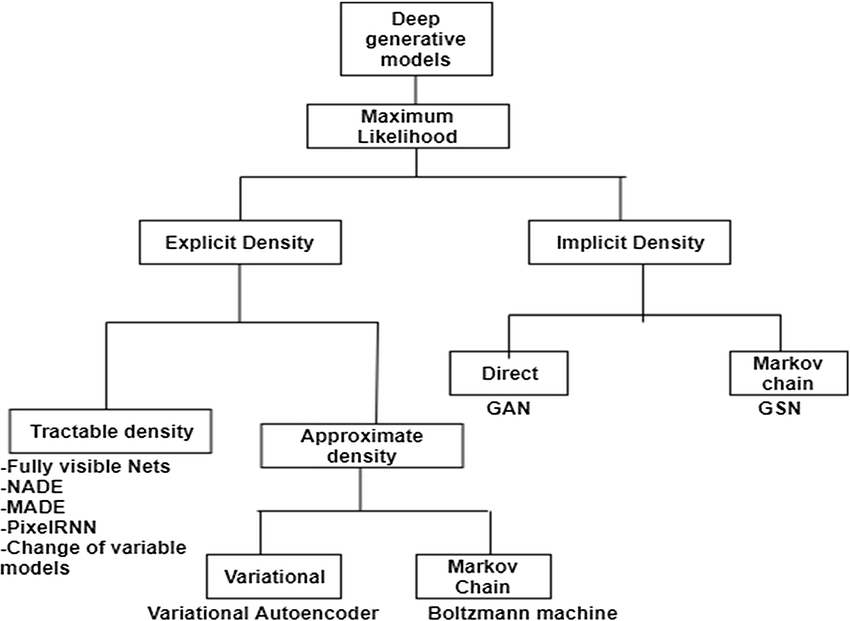
\includegraphics[width=\linewidth]{figures/intro/taxonomy-generative-models.png}
\caption{Taxonomy of Generative Models}
\label{fig:taxonomy_generative_models}

\end{figure}


Typical generative models are trained with maximum likelihood learning. The learnt density function can either be implicit as in the case of Generative Adversarial Networks\cite{goodfellow2014generative} and Generative Stochastic Networks \cite{alain2016gsns}. On the other hand the density can be explicitly modeled. Variational Autoencoders \cite{kingma2013auto} approximate the density function using the Evidence Lower Bound (ELBO). In case of autoregressive models such as PixelRNN\cite{van2016pixel} the density is tractable. Continuous Normalizing Flows \cite{chen2018neural, grathwohl2018ffjord} is also a form of explicit density estimation technique. 


Deep generative models models are function approximators, parametrized by a neural network with several layers. These networks are trained to approximate a complicated high dimensional probability distribution. On successful training, these trained models could either be used to estimate likelihood of a particular sample under the distribution. The trained deep generative model often allows us to draw samples from the distribution. Deep generative models has been one of the most active areas of research in recent years because of its incredible promise. Although, the promise hasn't been fulfilled and hence the increased research interest. In recent years three major avenues of deep generative model has taken centre-stage amongst many others. Variational Autoencoders(VAEs), Normalizing Flows(NFs) and Generative Adversarial Networks(GANs) are the ones that have shown the highest quality results. These are the models which have shown the highest resolution which can be potentially used for effective and reliable Visual Communication applications. 
 

\section{Applications of Generative Models for Visual Communication}
% Flesh it out with a bunch of images (wink visual communication)



\section{Challenges before Generative Models can become ubiquitous} 


\subsection{ Mode Collapse in GANs}

\subsection{ Improper Conditioning in Class Conditional GANs}

\subsection{ Assistance in Human Creativity}

\subsection{ Extremely slow training in Continuous Normalizing Flows}

\section{Approach}

\section{Structure of the thesis}



\chapter{MADGAN: Multi-Agent Diverse Generative Adversarial Networks
}

\begin{abstract}
	We propose MAD-GAN, an intuitive generalization to the Generative Adversarial Networks (GANs) and its {\em conditional variants} to address the well known problem of {\em mode collapse}. First, MAD-GAN is a multi-agent GAN architecture incorporating multiple generators and one discriminator. Second, to enforce that different generators capture diverse high probability modes, the discriminator of MAD-GAN is designed such that along with finding the real and fake samples, it is also required to identify the generator that generated the given fake sample. Intuitively, to succeed in this task, the discriminator must learn to push different generators towards different identifiable modes. 
	We perform extensive experiments on synthetic and real datasets and compare MAD-GAN with different variants of GAN. 
	We show high quality diverse sample generations for challenging tasks such as image-to-image translation and face generation. In addition, we also show that MAD-GAN is able to disentangle different modalities when trained using highly challenging diverse-class dataset (\eg the dataset with images of forests, icebergs, and bedrooms). In the end, we show its efficacy on the unsupervised feature representation task. In Appendix ~\ref{sec:competing}, we introduce a similarity based competing objective (MAD-GAN-Sim) which encourages different generators to generate diverse samples based on a user defined similarity metric. We show its performance on the image-to-image translation, and also show its effectiveness on the unsupervised feature representation task.
\end{abstract}


\section{Introduction}

Generative models have attracted considerable attention recently. The underlying idea behind such models is to attempt to capture the distribution of high-dimensional data such as images and texts. Though these models are highly useful in various applications, it is computationally expensive to train them as they require intractable integration in a very high-dimensional space. This drastically limits their applicability. However, recently there has been considerable progress in {\em deep generative models} -- conglomerate of deep neural networks and generative models -- as they do not explicitly require the intractable integration, and can be efficiently trained using back-propagation algorithm. Two such famous examples are Generative Adversarial Networks (GANs)~\cite{goodfellow2014generative} and Variational Autoencoders~\cite{kingma2013auto}.



In this paper we focus on GANs as they are known to produce sharp and plausible images. Briefly, GANs employ a generator and a discriminator where both are involved in a minimax game. The task of the discriminator is to learn the difference between {\em real} samples (from true data distribution $p_d$) and {\em fake} samples (from generator distribution $p_g$). Whereas, the task of the generator is to maximize the mistakes of the discriminator. At convergence, the generator learns to produce real looking images. A few successful applications of GANs are video generation~\cite{vondrick2016generating}, image inpainting~\cite{pathak2016context}, image manipulation~\cite{zhu2016generative}, 3D object generation~\cite{wu2016learning}, interactive image generation using few brush strokes~\cite{zhu2016generative}, image super-resolution~\cite{ledig2016photo}, diagrammatic abstract reasoning~\cite{ghosh2017contextual} and conditional GANs~\cite{mirza2014conditional,reed2016generative}.

Despite the remarkable success of GAN, it suffers from the major problem of {\em mode collapse}~\cite{arjovsky2016towards,che2016mode,chen2016infogan,metz2017unrolledGAN,salimans2016improved}. Though, theoretically, convergence guarantees the generator learning the true data distribution. However, practically, reaching the true equilibrium is difficult and not guaranteed, which potentially leads to the aforementioned problem of mode collapse. Broadly speaking, there are two schools of thought to address the issue: (1) improving the learning of GANs to reach better optima~\cite{arjovsky2016towards,metz2017unrolledGAN,salimans2016improved}; and (2) explicitly enforcing GANs to capture diverse modes~\cite{che2016mode,chen2016infogan,liu2016coupled}. Here we focus on the latter.


Borrowing from the multi-agent algorithm~\cite{abadi2016learning} and coupled GAN~\cite{liu2016coupled}, we propose to use multiple generators with one discriminator. We call this framework the Multi-Agent GAN architecture, as shown in Fig.~\ref{fig:multiAgentGAN}. In detail, similar to the standard GAN, the objective of each generator here is to maximize the mistakes of the {\em common} discriminator. Depending on the task, it might be useful for different generators to share information. This is done using the initial layer parameters of generators. Another reason behind sharing these parameters is the fact that initial layers capture low-frequency structures which are almost the same for a particular type of dataset (for example, faces), therefore, sharing them reduces redundant computations. However, when the dataset contains images from completely different modalities, one can avoid sharing these parameters. Naively using multiple generators may lead to the {\em trivial solution} where all the generators learn to generate {\em similar} samples. To resolve this issue and generate different visually plausible samples capturing diverse high probability modes, we propose to modify the objective function of the discriminator. In the modified objective, along with finding the real and the fake samples, the discriminator also has to correctly identify the generator that generated the given fake sample. Intuitively, in order to succeed in this task, the discriminator must learn to push generations corresponding to different generators towards different identifiable modes. Combining the Multi-Agent GAN architecture with the diversity enforcing term allows us to generate diverse plausible samples, thus the name Multi-Agent Diverse GAN (MAD-GAN).  


As an example, an intuitive setting where mode collapse occurs is when a GAN is trained on a dataset containing images from different modalities/classes. For example, a diverse-class dataset containing images such as forests, iceberg, and bedrooms. This is of particular interest as it not only requires the model to disentangle intra-class variations, it also requires inter-class disentanglement. Fig.~\ref{fig:madgan_multiview} demonstrates the surprising effectiveness of MAD-GAN in this challenging setting. Generators among themselves are able to disentangle inter-class variations, and each generator is also able to capture intra-class variations.

In addition, we analyze MAD-GAN through extensive experiments and compare it with several variants of GAN. First, for the proof of concept, we perform experiments in controlled settings using synthetic dataset (mixture of Gaussians), and complicated Stacked/Compositional MNIST datasets with hand engineered modes. In these settings, we empirically show that our approach outperforms all other GAN variants we compare with, and is able to generate high quality samples while capturing large number of modes. In a more realistic setting, we show high quality diverse sample generations for the challenging tasks of {\em image-to-image translation}~\cite{isola2016image2image} (conditional GAN) and {\em face generation}~\cite{chen2016infogan,radford2015unsupervised}. Using the SVHN dataset~\cite{Netzer11SVHN}, we also show the efficacy of our framework for learning the feature representation in an unsupervised setting.

We also provide theoretical analysis of this approach and show that the proposed modification in the objective of discriminator allows generators to learn together as a mixture model where each generator represents a mixture component. We show that at convergence, the global optimum value of $-(k+1)\log(k+1) + k \log k$ is achieved, where $k$ is the number of generators. 

\begin{figure}[ht]
	\centering
	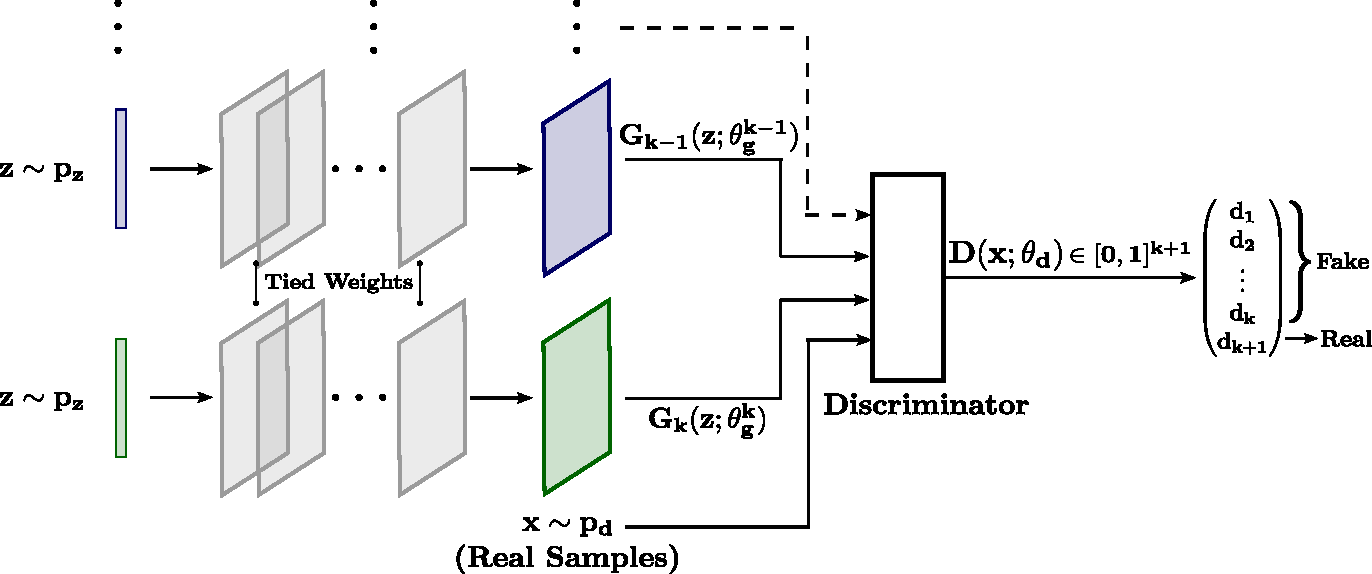
\includegraphics[scale=0.38]{Shared_MADGAN_GIO}
	\caption{Multi-Agent Diverse GAN (MAD-GAN). The discriminator outputs $k+1$ softmax scores signifying the probability of its input sample being from either one of the $k$ generators or the real distribution. 
	}
	\label{fig:multiAgentGAN}
	\vspace{-4mm}
\end{figure}
\section{Related Work}
The recent work called InfoGAN~\cite{chen2016infogan} proposed an information-theoretic extension to GANs in order to address the problem of mode collapse. Briefly, InfoGAN disentangles the latent representation by assuming a factored representation of the latent variables. In order to enforce that the generator learns factor specific generations, InfoGAN maximizes the mutual information between the factored latents and the generator distribution. 
Che \etal~\cite{che2016mode} proposed a mode regularized GAN (ModeGAN) which uses an encoder-decoder paradigm. The basic idea behind ModeGAN is that if a sample from the true data distribution $p_d$ belongs to a particular mode, then the sample generated by the generator (fake sample) when the true sample is passed through the encoder-decoder is likely to belong to the same mode. ModeGAN assumes that there exists enough true samples from a mode for the generator to be able to capture it.
Another work by Metz \etal~\cite{metz2017unrolledGAN} proposed a surrogate objective for the update of the generator with respect to the unrolled optimization of the discriminator (UnrolledGAN) to address the issue of convergence of the training process of GANs. This improves the training process of the generator which in turn allow the generators to explore better coverage to true data distribution. 

Liu \etal~\cite{liu2016coupled} presented Coupled GAN, a method for training two generators with shared parameters to learn the joint distribution of the data. The shared parameters guide both the generators towards similar subspaces but since they are trained independently on two domains, they promote diverse generations. Durugkar \etal~\cite{durugkar2016generative} proposed a model with multiple discriminators whereby an ensemble of multiple discriminators have been shown to stabilize the training of the generator by guiding it to produce better samples. 

W-GAN~\cite{arjovsky2017wasserstein} is a recent technique which employs integral probability metrics based on the earth mover distance rather than the JS-divergences that the original GAN uses. BEGAN~\cite{berthelot2017began} builds upon W-GAN using an autoencoder based equilibrium enforcing technique alongside the Wasserstein distance. DCGAN~\cite{radford2015unsupervised} was a seminal technique which used a fully convolutional generator and discriminator for the first time along with the introduction of batch normalization thus stabilizing the training procedure, and was able to generate compelling generations. GoGAN~\cite{juefei2017gang} introduced a training procedure for the training of the discriminator using a maximum margin formulation alongside the earth mover distance based on the Wasserstein-1 metric.~\cite{arora2017generalization} introduced a technique and theoretical formulation stating the importance of multiple generators and discriminators in order to completely model the data distribution. In terms of employing multiple generators, our work is closest to~\cite{arora2017generalization,liu2016coupled,ghosh2016message}. However, while using multiple generators, our method explicitly enforces them to capture diverse modes. 

\section{Preliminaries}
Here we present a brief review of GANs~\cite{goodfellow2014generative}. Given a set of samples $\mathcal{D} = (x_i)_{i=1}^n$ from the true data distribution $p_d$, the GAN learning problem is to obtain the optimal parameters $\theta_g$ of a generator $G(z;\theta_g)$ that can sample from an approximate data distribution $p_g$, where $z \sim p_z$ is the prior input noise (\eg samples from a normal distribution). In order to learn the optimal $\theta_g$, the GAN objective (Eq.~\eqref{eq:ganObjective}) employs a discriminator $D(x; \theta_d)$ that learns to differentiate between a {\em real} (from $p_d$) and a {\em fake} (from $p_g$) sample $x$. The overall GAN objective is:
\begin{align}
	\label{eq:ganObjective}
	\min_{\theta_g}\max_{\theta_d}\; & V(\theta_d, \theta_g) := \E_{x \sim p_{d}} \log D(x; \theta_d) \nonumber \\&
	+ \E_{z \sim p_z } \log \big( 1 - D(G(z; \theta_g) ; \theta_d)\big) 
\end{align}

The above objective is optimized in a block-wise manner where $\theta_d$ and $\theta_g$ are optimized one at a time while fixing the other. For a given sample $x$ (either from $p_d$ or $p_g$) and the parameter $\theta_d$, the function $D(x; \theta_d) \in [0, 1]$ produces a score that represents the probability of $x$ belonging to the true data distribution $p_d$ (or probability of it being real). The objective of the discriminator is to learn parameters $\theta_d$ that maximizes this score for the true samples (from $p_d$) while minimizing it for the fake ones $\tilde{x} = D(z; \theta_g)$ (from $p_g$). In the case of generator, the objective is to minimize $\E_{z \sim p_z}\log \big( 1 - D(G(z; \theta_g) ; \theta_d) \big)$, equivalently maximize $\E_{z \sim p_z} \log D(G(z; \theta_g) ; \theta_d)$. Thus, the generator learns to maximize the scores for the fake samples (from $p_g$), which is exactly the opposite to what discriminator is trying to achieve. In this manner, the generator and the discriminator are involved in a minimax game where the task of the generator is to maximize the mistakes of the discriminator. Theoretically, at equilibrium, the generator learns to generate real samples, which means $p_g = p_d$.

\section{Multi-Agent Diverse GAN}
In the GAN objective, one can argue that the task of a generator is much harder than that of the discriminator as it has to produce real looking images to maximize the mistakes of the discriminator. This, along with the minimax nature of the objective raise several challenges for GANs~\cite{arjovsky2016towards,che2016mode,chen2016infogan,metz2017unrolledGAN,salimans2016improved}: (1) mode collapse; (2) difficult optimization; and (3) trivial solution. In this work we propose a new framework to address the first challenge of {\em mode collapse} by increasing the capacity of the generator while using well known tricks to partially avoid other challenges~\cite{arjovsky2016towards}. 

Briefly, we propose a {\em Multi-Agent GAN architecture} that employs multiple generators and one discriminator in order to generate different samples from high probability regions of the true data distribution. 
In addition, theoretically, we show that our formulation allows generators to act as a mixture model with each generator capturing one component. 


\subsection{Multi-Agent GAN Architecture}
\label{subsection:architecture}
Here we describe our proposed architecture (Fig.~\ref{fig:multiAgentGAN}). It involves $k$ generators and one discriminator. In the case of homogeneous data (all the images belong to same class, \eg faces or birds), we allow all the generators to share information by tying most of the initial layer parameters. This is essential to avoid redundant computations as initial layers of a generator capture low-frequency structures which are almost the same for a particular type of dataset. This also allows different generators to converge faster. However, in the case of {\em diverse-class} data (\eg dataset with a mixture of different classes such as forests, icebergs \etc), it is necessary to avoid sharing these parameters to allow each generator to capture content specific structures. Thus, the extent to which one should share these parameters depends on the task at hand. 

More specifically, given $z \sim p_z$ for the $i$-th generator, similar to the standard GAN, the first step involves generating a sample (for example, an image) $\tilde{x}_i$. Since each generator receives the same latent input sampled from the same distribution, naively using this simple approach may lead to the {\em trivial solution} where all the generators learn to generate similar samples. In what follows, we propose an intuitive solution to avoid this issue and allow the generators to capture diverse modes.


\subsection{Enforcing Diverse Modes}
\label{sec:diverseModes}
\begin{figure}
	\centering
	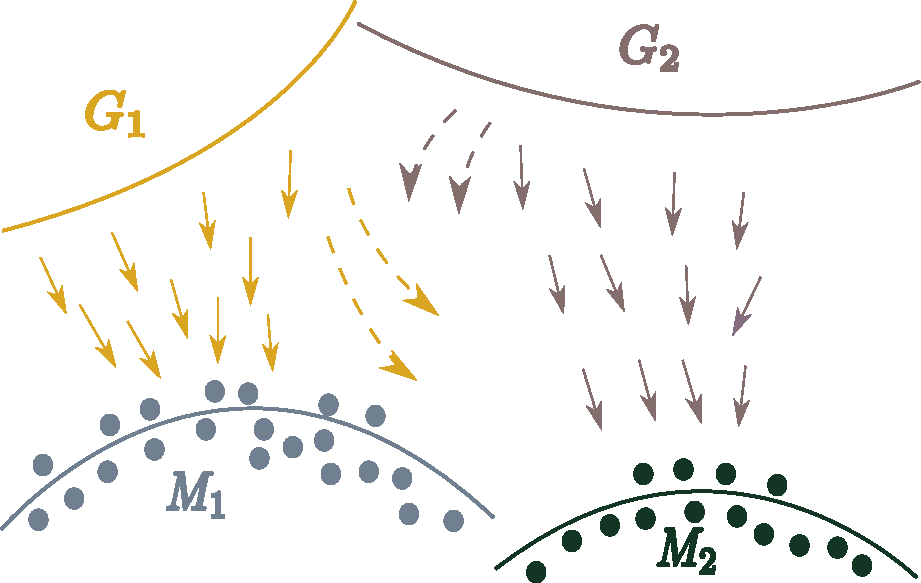
\includegraphics[width=0.5\linewidth]{multi-modes}
	\caption{Visualization of different generators getting pushed towards different modes. Here, $M_1$ and $M_2$ could be a cluster of modes where each cluster itself contains many modes. The arrows abstractly represent generator specific gradients for the purpose of building intuition.}
	\label{fig:modeVisualization}
	\vspace{-4mm}
\end{figure}

Inspired by the discriminator formulation for the semi-supervised learning~\cite{salimans2016improved}, we use a generator identification based objective function that, along with minimizing the score $D(\tilde{x}; \theta_d)$, requires the discriminator to identify the generator that generated the given fake sample $\tilde{x}$. In order to do so, as opposed to the standard GAN objective function where the discriminator outputs a scalar value, we modify it to output $k+1$ soft-max scores. In more detail, given the set of $k$ generators, the discriminator produces a soft-max probability distribution over $k+1$ classes.  The score at $(k+1)$-th index $(D_{k+1}(.))$ represents the probability that the sample belongs to the true data distribution and the score at $j \in \{1, \dots, k\}$-th index represents the probability of it being generated by the $j$-th generator. Under this setting, while learning $\theta_d$, we optimize the cross-entropy between the soft-max output of the discriminator and the Dirac delta distribution $\delta \in \{0,1\}^{k+1}$, where for $j \in \{1, \dots, k\}$, $\delta(j) = 1$ if the sample belongs to the $j$-th generator, otherwise $\delta(k+1) = 1$. Thus, the objective of the discriminator, which is optimizing $\theta_d$ while keeping $\theta_g$ constant (refer Eq.~(\ref{eq:ganObjective})), is modified to:
\begin{align*}
	\max_{\theta_d} \E_{x \sim p} H(\delta, D(x; \theta_d))
\end{align*}
where, $Supp(p) = \cup_{i=1}^k Supp(p_{g_i}) \cup Supp(p_d) $ and $H(.,.)$ is the negative of the cross entropy function. Intuitively, in order to correctly identify the generator that produced a given fake sample, the discriminator must learn to push different generators towards different identifiable modes. However, the objective of each generator remains the same as in the standard GAN. Thus, for the $i$-th generator, the objective is to minimize the following:
\begin{align}
	\mathbb{E}_{x\sim p_{d}}\log D_{k+1}(x; \theta_d) \hspace{-1mm}+ \hspace{-1mm}\mathbb{E}_{z \sim p_z}\log (1- D_{k+1}(G_i(z; \theta_g^i); \theta_d)) \nonumber
\end{align}
To update the parameters, the gradient for each generator is simply computed as $\nabla_{\theta_g^i} \log (1 - D_{k+1}(G_i(z; \theta_g^i); \theta_d)))$. Notice that all the generators in this case can be updated in parallel. For the discriminator, given $x \sim p$ (can be real or fake) and corresponding $\delta$, the gradient is $\nabla_{\theta_d}  \log D_j(x; \theta_d)$, where $D_j(x; \theta_d)$ is the $j$-th index of  $D(x; \theta_d)$ for which $\delta(j) = 1$. Therefore, using this approach requires {\em very minor modifications to the standard GAN optimization algorithm} and can be easily used with different variants of GAN. An intuitive visualization is shown in Fig.~\ref{fig:modeVisualization}.

Theorem~\ref{theo:optimalConditionGenId} shows that the above objective function actually allows generators to form a mixture model where each generator represents a mixture component and the global optimum of $-(k+1) \log (k+1) + k \log k$ is achieved when $p_d = \frac{1}{k} \sum_{i=1}^k p_{g_i}$. Notice that, at $k=1$, which is the case with one generator, we obtain exactly the same Jensen-Shannon divergence based objective function as shown in~\cite{goodfellow2014generative} with the optimal value of $-\log 4$.


\begin{theorem}
	\label{theo:optimalConditionGenId}
	Given the optimal discriminator, the objective for training the generators boils down to minimizing
	\begin{align}
		\label{eq:klDivProof}
		& KL \Big(p_d(x) ||  p_{avg}(x) \Big) + k KL \Big( \frac{1}{k} \sum_{i=1}^k p_{g_i} (x) ||  p_{avg}(x) \Big)  \nonumber \\
		&-(k+1) \log (k+1) + k \log k
	\end{align}
	where, $p_{avg} (x) = \frac{p_d(x) + \sum_{i=1}^k p_{g_i}(x)}{k+1}$. The above objective function obtains its global minimum if $p_d = \frac{1}{k} \sum_{i=1}^k p_{g_i}$ with the objective value of $-(k+1) \log (k+1) + k \log k$.
	\begin{proof}
		The joint objective of all the generators is to minimize the following:
		\begin{align}
			\mathbb{E}_{x\sim p_{d}}\log D_{k+1}(x) + \sum_{i=1}^{k}\mathbb{E}_{x \sim p_{g_i}}\log (1- D_{k+1}(x)) \nonumber 
		\end{align}
		Using Corollary~\ref{cor:optimalDiscrminator}, we substitute the optimal discriminator in the above equation and obtain:
		\begin{align}
			\label{eq:klDivFinal}
			& \mathbb{E}_{x\sim p_{d}}\log \Bigg [ \frac{p_d(x)}{p_d(x) + \sum_{i=1}^k p_{g_i}(x)} \Bigg]  + \nonumber \\
			&\sum_{i=1}^{k} \mathbb{E}_{x\sim p_{g_i}} \log \Bigg[ \frac{\sum_{i=1}^k p_{g_i}(x)}{p_d(x) + \sum_{i=1}^k p_{g_i}(x)} \Bigg] \nonumber \\
			&= \mathbb{E}_{x\sim p_{d}} \log \Bigg [ \frac{p_d(x)}{p_{avg}(x)} \Bigg]  + k \mathbb{E}_{x \sim p_g} \log \Bigg[ \frac{p_g(x)}{p_{avg}(x)} \Bigg] \nonumber \\
			&- (k+1) \log (k+1) + k \log k
		\end{align}
		where, $p_g=\frac{\sum_{i=1}^k p_{g_i}}{k}$ and $p_{avg} (x) = \frac{p_d(x) + \sum_{i=1}^k p_{g_i}(x)}{k+1}$. Note that, Eq.~(\ref{eq:klDivFinal}) is exactly the same as Eq.~(\ref{eq:klDivProof}). When $p_d = \frac{\sum_{i=1}^k p_{g_i}}{k}$, both the KL terms become zero and the global minimum is achieved. 
	\end{proof}
\end{theorem}

\begin{corollary}
	\label{cor:optimalDiscrminator}
	For fixed generators, the optimal distribution learned by the discriminator D has the following form:
	\begin{align*}
		D_{k+1}(x) &=  \frac{p_d(x)}{p_d(x) + \sum_{i=1}^k p_{g_i}(x)}, \\ \nonumber
		D_i(x) &=  \frac{p_{g_i}(x)}{p_d(x) + \sum_{i=1}^k p_{g_i}(x)}, \forall i \in \{1, \cdots, k\}.
	\end{align*}
	where, $D_i(x)$ represents the $i$-th index of $D(x; \theta_d)$, $p_d$ the true data distribution, and $p_{g_i}$ the distribution learned by the $i$-th generator.
	\begin{proof}
		For fixed generators, the objective function of the discriminator is to maximize
		\begin{align*}
			\mathbb{E}_{x\sim p_{d}}\log D_{k+1}(x) + \sum_{i=1}^{k}\mathbb{E}_{x_i\sim p_{g_i}}\log D_i (x_i) 
		\end{align*}
		where, $\sum_{i=1}^{k+1} D_i(x) = 1$ and $D_i(x) \in [0, 1], \forall i$. The above equation can be written as:
		\begin{align}
			\label{eq:optDis2}
			& \int_x p_d(x)\log D_{k+1} (x) dx + \sum_{i=1}^k\int_x p_{g_i}(x)\log D_i(x) dx \nonumber \\
			& = \int_{x \in p} \sum_{i=1}^{k+1} p_i(x) \log D_i(x) dx
		\end{align}
		where, $p_{k+1}(x) := p_d(x)$, $p_i(x) := p_{g_i} (x), \forall i \in \{1, \cdots, k\}$, and $Supp(p) = \bigcup_{i=1}^k Supp(p_{g_i}) \bigcup Supp(p_d)$,   Therefore, for a given $x$, the optimum of objective function defined in Eq.~(\ref{eq:optDis2}) with constraints defined above can be obtained using Proposition~\ref{prop:lpCons}.
	\end{proof}
\end{corollary}

\begin{proposition}
	\label{prop:lpCons}
	Given ${\bf y} = (y_1, \cdots, y_n)$, $y_i \geq 0$, and $a_i \in \mathbb{R}$, the optimal solution for the objective function defined below is achieved at $y_i^* = \frac{a_i}{\sum_{i = 1}^n a_i}, \forall i$
	\begin{align*}
		\max_{\bf y} \sum_{i=1}^n a_i\log y_i,  \;\; s.t. \; \sum_i^n y_i = 1
	\end{align*}
	\begin{proof}
		The Lagrangian of the above problem is:
		\begin{align*}
			L({\bf y}, \lambda) = \sum_{i=1}^n a_i\log y_i + \lambda (\sum_{i=1}^n y_i - 1) 
		\end{align*}
		Differentiating w.r.t $y_i$ and $\lambda$, and equating to zero,
		\begin{align*}
			\frac{a_i}{y_i} + \lambda = 0 \; , \; \sum_{i=1}^n y_i - 1 = 0
		\end{align*}
		Solving the above two equations, we obtain $y_i^* = \frac{a_i}{\sum_{i = 1}^n a_i}$.
	\end{proof}
\end{proposition}

\newcommand{\addSubFig}[3]{\begin{subfigure}[t]{.33\linewidth}
		\includegraphics[width=\linewidth]{#1}
		\caption{#2}\label{#3}\end{subfigure}
}

%% 1D experiments
\newcommand{\addSubFigEighth}[3]{\begin{subfigure}[t]{.24\linewidth}
		\includegraphics[width=\linewidth]{#1}
		\caption{#2}\label{#3}\end{subfigure}
}

\newcommand{\addSubFigNineth}[3]{\begin{subfigure}[t]{.19\linewidth}
		\includegraphics[width=\linewidth]{#1}
		\caption{#2}\label{#3}\end{subfigure}
}

%% 1D experiments
\begin{figure}
	\centering
	\addSubFigNineth{DCGAN_1D}{DCGAN}{fig:DCGAN_1D} 
	\addSubFigNineth{WGAN_1D}{WGAN}{fig:WGAN_1D} 
	\addSubFigNineth{BEGAN_1D}{BEGAN}{fig:BEGAN_1D} 
	\addSubFigNineth{GGAN_2nd_1D}{GoGAN}{fig:GoGAN_1D}\\ 
	\addSubFigNineth{UNROLLEDGAN_1D}{Unrolled GAN}{fig:Unrolled_1D} 
	\addSubFigNineth{MODEGAN_1D}{Mode-Reg DCGAN}{fig:ModeReg_1D} 
	\addSubFigNineth{InfoGAN_1D}{InfoGAN}{fig:InfoGAN_1D} 
	\addSubFigNineth{TRIVIAL_1D}{MA-GAN}{fig:MA-GAN_1D} 
	\addSubFigNineth{MADGAN_1D}{MAD-GAN (Our)}{fig:MAD-GAN_1D} 
	\caption{A toy example to understand the behaviour of different GAN variants in order to compare with MAD-GAN (each method was trained for 198000 iterations).  The orange bars show the density estimate of the training data and the blue ones for the generated data points. After careful cross-validation, we chose the bin size of $0.1$. }
	\label{fig:toy_1D}
	\vspace{-3mm}
\end{figure}

\begin{figure}
	\centering
	\addSubFigEighth{MADGAN_1_1D}{1 Generator}{fig:MADGAN_1} 
	\addSubFigEighth{MADGAN_2_1D}{2 Generators}{fig:MADGAN_2} 
	\addSubFigEighth{MADGAN_3_1D}{3 Generators}{fig:MADGAN_3} 
	\addSubFigEighth{MADGAN_4_1D}{4 Generators}{fig:MADGAN_4}\\ 
	\addSubFigEighth{MADGAN_5_1D}{5 Generators}{fig:MADGAN_5} 
	\addSubFigEighth{MADGAN_6_1D}{6 Generators}{fig:MADGAN_6} 
	\addSubFigEighth{MADGAN_7_1D}{7 Generators}{fig:MADGAN_7} 
	\addSubFigEighth{MADGAN_8_1D}{8 Generators}{fig:MADGAN_8} 
	\caption{A toy example to understand the behavior of MAD-GAN with different number of generators (each method was trained for $1,98,000$ iterations).  The orange bars show the density estimate of the training data and the blue ones for the generated data points. After careful cross-validation, we chose the bin size of $0.1$. }
	\label{fig:toy_1D_multi}
	\vspace{-3mm}
\end{figure}

\section{Experiments}
We present an extensive quantitative and qualitative analysis of MAD-GAN on various synthetic and real-world datasets. First, we use a simple 1D mixture of Gaussians and also Stacked/Compositional MNIST dataset (1000 modes) to compare MAD-GAN with several known variants of GANs, such as DCGAN \cite{radford2015unsupervised}, WGAN \cite{arjovsky2017wasserstein}, BEGAN \cite{berthelot2017began}, GoGAN \cite{juefei2017gang}, Unrolled GAN \cite{metz2017unrolledGAN}, Mode-Reg GAN \cite{che2016mode} and InfoGAN \cite{chen2016infogan}. Furthermore, we created another baseline, called {\em MA-GAN (Multi-Agent GAN)}, which is a trivial extension of GAN with multiple generators and one discriminator. As opposed to MAD-GAN, MA-GAN has a simple Multi-Agent architecture without modifications to the objective of the discriminator. This comparison allows us to understand the effect of explicitly enforcing diversity in the objective of the MAD-GAN. We use KL-divergence \cite{kullback1951information} and number of modes recovered \cite{che2016mode} as the criterion for comparisons and show superior results compared to all the other methods. Additionally, we show diverse generations for the challenging tasks of {\em image-to-image translation}~\cite{isola2016image2image}, {\em diverse-class data generation}, and face generation. It is non-trivial to devise a metric to evaluate diversity on these high quality generation tasks, so we perform qualitative assessment. Note that, the image-to-image translation objective is known to learn the delta distribution, thus, it is agnostic to the input noise vector. However, we show that MAD-GAN is able to produce highly plausible diverse generations for this task. In the end, we show the efficacy of MAD-GAN in unsupervised feature representation learning task. We provide detailed overview of the architectures, datasets, and the parameters used in our experiments in the Appendix~\ref{sec:architectures}.

In the case of InfoGAN~\cite{chen2016infogan}, we varied the dimension of the categorical variable, depicting the number of modes, to obtain the best cross-validated results.


\begin{table}
	\centering
	\begin{tabular}{c@{\hspace{2pt}}c@{\hspace{4pt}}c}
		\toprule
		\textbf{GAN Variants} & \textbf{Chi-square}${(\times10^5)}$ & \textbf{KL-Div} \\
		\midrule
		DCGAN~\cite{radford2015unsupervised} & 0.90  & 0.322\\ 
		WGAN~\cite{arjovsky2017wasserstein} & 1.32 & 0.614\\ 
		BEGAN~\cite{berthelot2017began} & 1.06 & 0.944\\ 
		GoGAN~\cite{juefei2017gang} & 2.52 & 0.652\\
		Unrolled GAN~\cite{metz2017unrolledGAN} & 3.98 & 1.321 \\ 
		Mode-Reg DCGAN~\cite{che2016mode}  & 1.02 & 0.927 \\ 			
		InfoGAN~\cite{chen2016infogan}  & 0.83 & 0.21 \\ 
		MA-GAN & 1.39 & 0.526 \\
		\textbf{MAD-GAN (Our)} &  \textbf{0.24} & \textbf{0.145}\\ 
		\bottomrule
	\end{tabular}
	\caption{\label{tab:toy_1D}Synthetic experiment on 1D GMM (Fig.~\ref{fig:toy_1D}).}
	\vspace{-1mm}
\end{table}


\begin{table}
	\centering
	\begin{tabular}{c@{\hspace{8pt}}c@{\hspace{8pt}}c} 
		\toprule
		\textbf{\# Generators} & \textbf{Chi-square} ${(\times10^7)}$ & \textbf{KL-Div} \\
		\midrule
		1 & 1.27  & 0.57\\ 
		2 & 1.38 & 0.42\\ 
		3 & 3.15 & 0.71\\
		4 & 0.39 & 0.28\\
		5 & 3.05 & 0.88\\
		6 & 0.54 & 0.29\\
		7 & 0.97 & 0.78\\
		8 & 4.83 & 0.68\\
		\bottomrule
	\end{tabular}
	\caption{\label{tab:toy_1D_multi}Synthetic experiment with different number of MAD-GAN generators (same setup as in Fig.~\ref{fig:toy_1D}).}
	\vspace{-3mm}
\end{table}

\subsection{Non-Parametric Density Estimation}
\label{sec:toyExperiment}
In order to understand the behavior of MAD-GAN and different state-of-the-art GAN models, we first perform a very simple synthetic experiment, much easier than generating high-dimensional complex images. We consider a distribution of 1D GMM~\cite{bishop2007pattern} having five mixture components with modes at 10, 20, 60, 80 and 110, and standard deviations of 3, 3, 2, 2 and 1, respectively. While the first two modes overlap significantly, the fifth mode stands isolated as shown in Fig.~\ref{fig:toy_1D}. We train different GAN models using $200,000$ samples from this distribution and generate $65,536$ data points from each model. In order to compare the learned distribution with the ground truth distributions, we first estimate them using bins over the data points and create the histograms. These histograms are carefully created using different bin sizes and the best bin (found to be $0.1$) is chosen. Then, we use Chi-square distance and the KL-divergence to compute distance between the two histograms. From Fig.~\ref{fig:toy_1D} and Tab.~\ref{tab:toy_1D} it is evident that MAD-GAN is able to capture all the clustered modes which includes significantly overlapped modes as well. MAD-GAN obtains the minimum value in terms of both Chi-square distance and the KL-divergence. In this experiment, both MAD-GAN and MA-GAN used four generators. In the case of InfoGAN, we used $5$ dimensional categorical variable, which provides the best result. 

To understand the effect of varying the number of generators in MAD-GAN, we use the same synthetic experimental setup, \ie the real data distribution is the same GMM with $5$ Gaussians. For better non-parametric estimation of the distribution, we use $1$ million sample points from the real distribution (instead of $65,536$). We generate an equal number of points from each of the generators such that they sum up to $1$ million. The results are shown in Fig.~\ref{fig:toy_1D_multi} and corresponding Tab.~\ref{tab:toy_1D_multi}. It is quite clear that as the number of generators are increased up to $4$, the sampling keeps getting more realistic. In the case when multiple modes are significantly overlapped/clustered, a generator can capture a cluster of modes. Therefore, for this real data distribution, $4$ generators are enough to capture all the $5$ modes. With $5$ or more generators, all the modes were still captured, but the two overlapping modes have more than two generation peaks. This is mainly because multiple generators capture this region and all the generators (mixture components) were assigned {\em equal weights} during sampling.

Other work using more than one generators~\cite{liu2016coupled, arora2017generalization} also use the number of generators as a hyper-parameter as knowing a-priori the number of modes in a real-world data (\eg images) in itself is an open problem.


\begin{table}
	\centering
	\begin{tabular}{c@{\hspace{2pt}}c@{\hspace{8pt}}c} 
		\toprule
		\textbf{GAN Variants} & \textbf{KL Div} & \textbf{\# Modes Covered} \\
		\midrule
		DCGAN~\cite{radford2015unsupervised}  & 2.15  & 712\\ 
		WGAN~\cite{arjovsky2017wasserstein}  & 1.02 & 868 \\ 
		BEGAN~\cite{berthelot2017began}  & 1.89 & 819\\ 
		GoGAN~\cite{juefei2017gang}  & 2.89 & 672\\
		Unrolled GAN~\cite{metz2017unrolledGAN} &1.29 & 842\\ 
		Mode-Reg DCGAN~\cite{che2016mode}  & 1.79 & 827 \\ 
		InfoGAN~\cite{chen2016infogan}  & 2.75 & 840 \\ 
		MA-GAN & 3.4 & 700 \\
		\textbf{MAD-GAN (Our)} &  \textbf{0.91} & \textbf{890}\\ 
		\bottomrule		
	\end{tabular}
	\caption{\label{tab:stacked_mnist}Stacked-MNIST experiments and comparisons. Note that three generators are used for MAD-GAN.
	}
	\vspace{-3mm}
\end{table}


\begin{table}
	\centering
	\begin{tabular}{c@{\hspace{2pt}}c@{\hspace{8pt}}c} 
		\toprule
		\textbf{GAN Variants} & \textbf{KL Div} & \textbf{\# Modes Covered} \\
		\midrule
		DCGAN~\cite{radford2015unsupervised}  & 0.18  & 980\\ 
		WGAN~\cite{arjovsky2017wasserstein} & 0.25 & 1000\\ 
		BEGAN~\cite{berthelot2017began} & 0.19 & 999\\ 
		GoGAN~\cite{juefei2017gang} & 0.87 & 972\\
		Unrolled GAN~\cite{metz2017unrolledGAN} &0.091 & 1000 \\
		Mode-Reg DCGAN~\cite{che2016mode}  & 0.12 & 992 \\ 
		InfoGAN~\cite{chen2016infogan}  & 0.47 & 990 \\ 
		MA-GAN & 1.62 & 997 \\
		\textbf{MAD-GAN (Our)} &  \textbf{0.074} & \textbf{1000}\\ 
		\bottomrule
	\end{tabular}
	\caption{\label{tab:compositional_mnist}Compositional-MNIST experiments and comparisons. Note that three generators are used for MAD-GAN.
	}
	\vspace{-3mm}
\end{table}

\newcommand{\addSubFigHalf}[2]{\begin{subfigure}{.48\linewidth}
		\centering
		\includegraphics[width=.88\linewidth]{#1}
		\label{#2}\end{subfigure}
}

\begin{figure*}
	\centering
	\addSubFigHalf{pix2pix_bags1}{fig:bags1} 
	\addSubFigHalf{pix2pix_bags2}{fig:bags2} \\
	\captionof{figure}{Diverse generations for {\em edges-to-handbags} generation task. In each sub-figure, the first column is the input, columns 2-4 are generations by MAD-GAN (using three generators), and columns 5-7 are generations by InfoGAN (using three categorical codes). Clearly different generators of MAD-GAN are producing diverse results capturing different colors, textures, design patterns, \etc. However, InfoGAN generations are visually almost the same, indicating mode collapse.
	}\label{fig:pix2pixBag}
	\vspace{-2mm}
\end{figure*}

\begin{figure*}
	\centering
	\addSubFigHalf{InfoGAN_bags1}{fig:infobags1} 
	\addSubFigHalf{InfoGAN_bags2}{fig:infobags2} \\
	\captionof{figure}{InfoGAN for {\em edges-to-handbags} task by sharing the discriminator and Q Network. In each sub-figure, the first column is the input, columns $2-4$ are generations when input is categorical code besides conditioning image, and columns $5-7$ are generations with noise as an additional input. The generations for both the architectures are visually the same irrespective of the categorical code value, which clearly indicates that it is not able to capture diverse modes.
	}\label{fig:pix2pixBag_infoGAN}
	\vspace{-3mm}
\end{figure*}

\subsection{Stacked and Compositional MNIST}
We now perform experiments on a more challenging setup, similar to~\cite{che2016mode,metz2017unrolledGAN}, in order to examine and compare MAD-GAN with other GAN variants. \cite{metz2017unrolledGAN} created a Stacked-MNIST dataset with $25,600$ samples where each sample has three channels stacked together with a random MNIST digit in each of them. Thus, it creates $1000$ distinct modes in the data distribution. \cite{metz2017unrolledGAN} used a stripped down version of the generator and discriminator pair to reduce the modeling capacity. We do the same for fair comparisons and used the same architecture as mentioned in their paper. Similarly, \cite{che2016mode} created Compositional-MNIST whereby they took $3$ random MNIST digits and place them at the $3$ quadrants of a $64 \times 64$ dimensional image. This also resulted in a data distribution with $1000$ hand-designed modes. The distribution of the resulting generated samples was estimated using a pretrained MNIST classifier to classify each of the digits either in the channels or the quadrants to decide the mode it belongs to. 

Tables~\ref{tab:stacked_mnist} and~\ref{tab:compositional_mnist} provide comparison of our method with variants of GAN in terms of KL divergence and the number of modes recovered for the Stacked and Compositional MNIST datasets, respectively. In Stacked-MNIST, as evident from the Tab.~\ref{tab:stacked_mnist}, MAD-GAN outperforms all other variants of GAN in both the criteria. Interestingly, in the case of Compositional-MNIST, as shown in Tab.~\ref{tab:compositional_mnist}, MAD-GAN, WGAN and Unrolled GAN were able to recover all the $1000$ modes. However, in terms of KL divergence, the distribution generated by MAD-GAN is the closest to the true data distribution.


\begin{figure}
	\centering
	\addSubFigHalf{day1_classifying}{fig:nightCom} 
	\addSubFigHalf{day2_classifying}{fig:nightGen} 
	\captionof{figure}{Diverse generations for {\em night-to-day} image generation task. First column in each sub-figure represents the input. The remaining three columns show the diverse generations of three different generators of MAD-GAN (Our). 
	}\label{fig:image2imageNight}
	\vspace{-4mm}
\end{figure}

\newcommand{\addSubFigThird}[2]{\begin{subfigure}{.31\linewidth}
		\centering
		\includegraphics[width=\linewidth]{#1}
		\label{#2}\vspace{-3mm}\end{subfigure}
}

\begin{figure*}
	\centering
	\addSubFigThird{faces_gen1}{fig:fg1} 
	\addSubFigThird{faces_gen2}{fig:fg2}
	\addSubFigThird{faces_gen3}{fig:fg3}
	\captionof{figure}{Face generations using MAD-GAN. Each sub-figure shows generations by a single generator. The first generator is generating faces with very dark background. The second one is generating female faces with long hair in light background, while the third one is generating faces with colored background and casual look (based on facial direction and expression).
	}\label{fig:faces}
	\vspace{-3mm}
\end{figure*}

\subsection{Diverse Samples for Image-to-Image Translation and Comparison to InfoGAN}
Here we present experimental results on the challenging task of image-to-image translation~\cite{isola2016image2image} which uses conditional variant of GANs~\cite{mirza2014conditional}. Conditional GAN for this task is known to learn the delta distribution, thus, generates the same image irrespective of the variations in the input noise vector. Generating diverse samples in this setting in itself is an open problem. We show that MAD-GAN is able to generate diverse samples in these experiments as well. We use three generators for MAD-GAN experiments and show three diverse generations. Note that, we do not claim to capture all the possible modes present in the data distribution because firstly we cannot estimate the number of modes a priori, and secondly, even if we could, we do not know how diverse the generations would be after using certain number of generators. 
We follow the same approach as~\cite{isola2016image2image} and employ patch based conditional GAN. 

We compare MAD-GAN with InfoGAN~\cite{chen2016infogan} in these experiments as it is closest to our approach and can be used in image-to-image translation task. Theoretically, latent codes in InfoGAN should enable diverse generations. However, InfoGAN can only be used when the bias introduced by the categorical variables have significant impact on the generator network. For image-to-image translation and high resolution generations, the categorical variable does not have sufficient impact on the generations. As will be seen shortly, we validate this hypothesis by comparing our method with InfoGAN for this task. 
For the InfoGAN generator, to capture three kinds of distinct modes, the categorical code is chosen to take three values. Since we are dealing with images, in  this case, the categorical code is a 2D matrix in which we set one third of the entries to 1 and remaining to 0 for each category. The generator is fed input image along with categorical code appended channel wise to the image. Architecture of the Q network is same as that of the pix2pix discriminator~\cite{isola2016image2image}, except that the output is a vector of size $3$ for the prediction of the categorical codes. Note that, we tried different variations of the categorical codes but did not observe any significant variation in the generations.

Fig.~\ref{fig:pix2pixBag} shows generations by MAD-GAN and InfoGAN for the {\em edges-to-handbags} task, where given the edges of handbags, the objective is to generate real looking handbags. Clearly, each MAD-GAN generator is able to produce meaningful images but different from remaining generators in terms of color, texture, and patterns. However, InfoGAN generations are almost the same for all the three categorical codes. The results shown for InfoGAN are obtained by not sharing the discriminator and Q network parameters.

To make our baseline as strong as possible, we did some more experiments with InfoGAN for the {\em edges-to-handbags} task. For Fig.~\ref{fig:pix2pixBag_infoGAN}, we conducted two experiments by sharing all the initial layers of the discriminator and Q network. In the first experiment, the input is the categorical code besides the conditional image. In the second experiment, noise is also added as an input. The details of the architecture are given in Appendix~\ref{subsection:InfoArch}. In Fig.~\ref{fig:pix2pixBag_infoGAN}, we show the results of both these experiments side by side. There are not many perceivable changes as we vary the categorical code values, as the generator learns to ignore the input noise (as was also seen in~\cite{isola2016image2image}).

In addition, in Fig.~\ref{fig:image2imageNight}, we show diverse generations for the {\em night-to-day} task, where given night images, the objective is to generate their corresponding day images. As can be seen, the generated day images in Fig.~\ref{fig:image2imageNight} differ in terms of lighting conditions, sky patterns, weather conditions, and many other minute yet useful cues. 


\newcommand{\addSubFigDCGAN}[3]{\begin{subfigure}[t]{.7\linewidth}
		\includegraphics[width=\linewidth]{#1}
		\caption{#2}\label{#3}\end{subfigure}
}
\begin{figure}
	\centering
	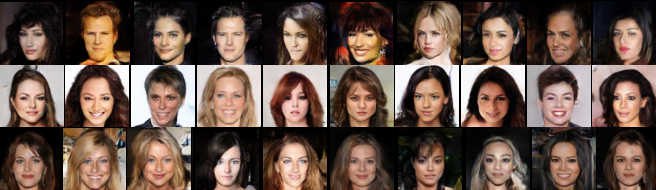
\includegraphics[width=\linewidth]{madgan_faces}
	\caption{Face generations using MAD-GAN. Each generator employed is DCGAN. Each row represents a generator. Each column represents generations for a given random noise input $z$. Note that, the first generator is generating faces pointing to the left. The second generator is generating female faces with long hair, while the third generator generates images with light background. 
	}
	\label{fig:DCGANfaces}
	\vspace{-4mm}
\end{figure}


\subsection{Diverse-Class Data Generation}
To further explore the mode capturing capacity of MAD-GAN, we experimented with a much more challenging task of diverse-class data generation. In detail, we trained MAD-GAN (three generators) on a combined dataset consisting of various highly diverse images such as {\em islets}, {\em icebergs}, {\em broadleaf-forest}, {\em bamboo-forest}, and {\em bedroom}, obtained from the Places dataset~\cite{zhou2017places}. Images were randomly selected from each of them, creating a training dataset of $24,000$ images. The generators have the same architecture as that of DCGAN. In this case, as the images in the dataset belong to different classes, we did not share the generator parameters. As shown in Fig.~\ref{fig:madgan_multiview}, to our surprise, we found that even in this highly challenging setting, the generations from different generators belong to different classes. This clearly indicates that the generators in MAD-GAN are able to disentangle inter-class variations. In addition, each generator for different noise input is able to generate diverse samples, indicating intra-class diversity. 

\subsection{Diverse Face Generation}
Here we show diverse face generations (CelebA dataset) using MAD-GAN where we use DCGAN~\cite{radford2015unsupervised} as each of our three generators. Again, we use the same setting as provided in DCGAN. The high quality face generations are shown in the Fig.~\ref{fig:DCGANfaces}. We show additional generations in Fig.~\ref{fig:faces}.

\subsection{Unsupervised Representation Learning}
\label{subsec:unsup_svhn}
Similar to DCGAN~\cite{radford2015unsupervised}, we train our framework using SVHN dataset~\cite{Netzer11SVHN}. The trained discriminator is used to extract features. Using these features, we train an SVM for the classification task. For the MAD-GAN, with three generators, we obtained misclassification  error of $17.5 \%$ which is almost $5\%$ better than the results reported by DCGAN ($22.48 \%$). This clearly indicates that our framework is able to learn a better feature space in an unsupervised setting. 

\section{Conclusion}
We presented a very simple and effective framework, Multi-Agent Diverse GAN (MAD-GAN), for generating diverse and meaningful samples. We showed the efficacy of our approach and compared it with various variants of GAN that it captures diverse modes while producing high quality samples. We presented a theoretical analysis of MAD-GAN with conditions for global optimality. Looking forward, an interesting future direction would be to estimate a priori the number of generators needed for a particular dataset. It is not clear how to do that given that we do not have access to the true data distribution. In addition, we would also like to theoretically understand the limiting cases that depend on the relationship between the number of generators and the complexity of the data distribution. Another interesting direction would be to exploit different generators such that their combinations can be used to capture diverse modes. 

\section{Acknowledgements}
This work was supported by the EPSRC, ERC grant ERC-2012-AdG 321162-HELIOS, EPSRC grant Seebibyte EP/M013774/1 and EPSRC/MURI grant EP/N019474/1.

{\small
	\bibliographystyle{ieee}
	\bibliography{biblio}
}

\newpage
% \appendix

\section{Appendix}
Here, we first give better insights about the Theorem~\ref{theo:optimalConditionGenId} and discuss how and when MAD-GAN leads to diverse generations. In Appendix~\ref{sec:competing}, we introduce another way of getting different generators to generate diverse samples. We introduce intuitive similarity based competing objective (MAD-GAN-Sim) which encourages different generators to generate diverse samples. Finally in Appendix~\ref{sec:architectures}, we provide architecture details and data preparations for all the experiments reported for MAD-GAN and MAD-GAN-Sim.

\section{Insights for Diversity in MAD-GAN}
One obvious question that could arise is that {\em is it possible that all the generators learn to capture the same mode?}. The short answer is, theoretically {\em yes} and in practice {\em no}. Let us begin with the discussion to understand this. Theoretically, according to Theorem~\ref{theo:optimalConditionGenId} if $p_{g_i} = p_d$, for all $i$, then also the minimum objective value can be achieved. This implies, in worst case, MAD-GAN would perform same as the standard GAN. However, as discussed below, this is possible in following {\em highly unlikely} situations:
\begin{itemize}
	\item all the generators {\em always generate exactly similar} samples so that the discriminator is not able to differentiate them. In this case, the discriminator will learn a uniform distribution over the generator indices, thus, the gradients passed through the discriminator will be exactly the same for all the generators. However, this situation in general is not possible as all the generators are initialized differently. Even a slight variation in the samples from the generators will be enough for the discriminator to identify them and pass different gradient information to each generator. In addition, the objective function of generators is {\em only} to generate {\em real} samples, thus, there is nothing that encourages them to generate exactly the same samples. 
	\item the discriminator does not have enough capacity to learn the optimal parameters. This is in contrast to the assumption made in Theorem 1, which is that the discriminator is {\em optimal}. Thus, it should have enough capacity to learn a feature representation such that it can correctly identify samples from different generators. In practice, this is a very easy task and we did not have to modify anything up to the feature representation stage of the architecture of the discriminator. We used the standard architectures (explained in Appendix~\ref{sec:architectures}) for all the tasks. 
\end{itemize}
Hence, with random initializations and sufficient capacity generator/discriminator, we can easily avoid the trivial solution in which all the generators focus on exactly the same region of the true data distribution. This has been very clearly supported by various experiments showing diverse generations by MAD-GAN. 

\section{Similarity based competing objective}
\label{sec:competing}
We have discussed the MAD-GAN architecture using generator identification based objective. In this section, we propose a different extension to the standard GAN : {\em similarity based competing objective}, which we call as MAD-GAN-Sim. Here, we augment the GAN objective function with a diversity enforcing term. It ensures that the generations from different generators are diverse where the diversity depends on a user-defined task-specific function.

The architecture is same as that of MAD-GAN discussed in Section~\ref{subsection:architecture} (refer Fig.~\ref{fig:multiAgentGAN_both}).

\begin{figure}[ht]
	\centering
	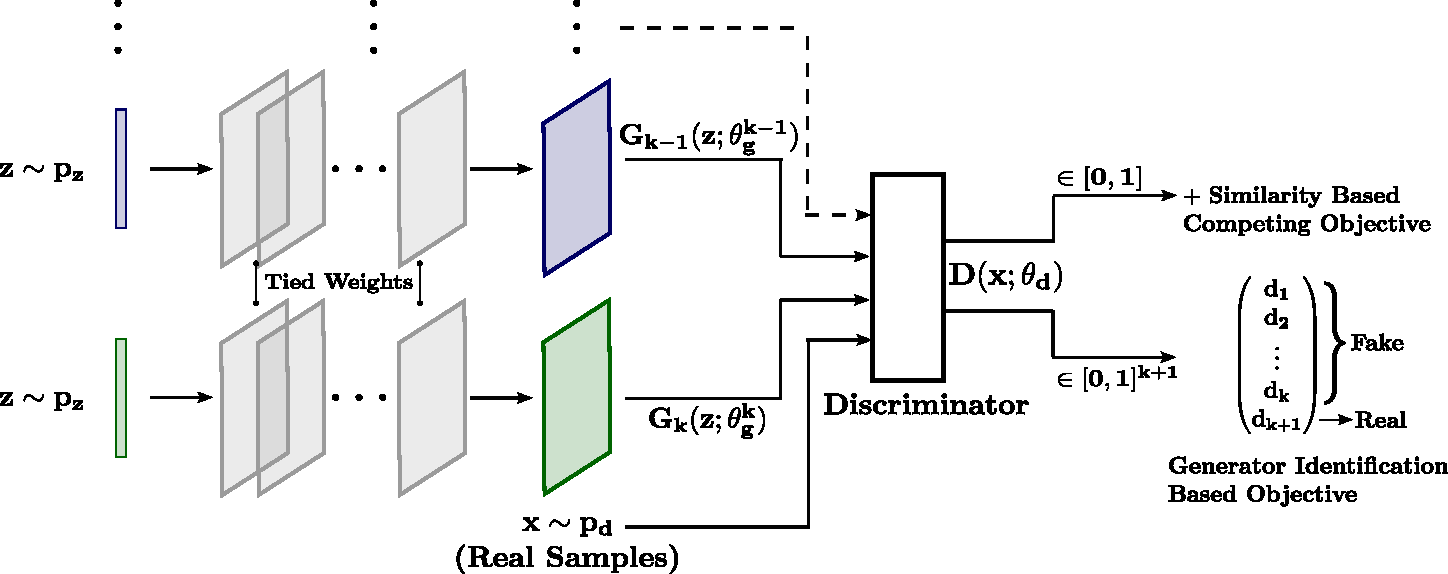
\includegraphics[scale=0.35]{Shared_MADGAN_both}
	\caption{MAD-GAN-Sim compared with MAD-GAN. All the generators share parameters of all the layers except the last one. The two proposed diversity enforcing objectives, `competing' (MAD-GAN-Sim) and `generator identification' (MAD-GAN), are shown at the end of the discriminator}
	\label{fig:multiAgentGAN_both}
\end{figure}

\subsection{Approach}
The approach presented here is motivated by the fact that the samples from different modes must look different. For example, in the case of images, these samples should differ in terms of texture, color, shading, and various other cues. Thus, different generators must generate dissimilar samples where the dissimilarity comes from a task-specific function. Before delving into the details, let us first define some notations in order to avoid clutter. We denote $\theta_g^i$ as the parameters of the $i$-th generator. The set of generators is denoted as $K = \{1, \cdots, k\}$. Given a random noise $z$ to the $i$-th generator, the corresponding generated sample $G_i(z; \theta_g^i)$ is denoted as $g_i(z)$. Using these notations and following the above discussed intuitions, we impose following constraints over the $i$-th generator while updating its parameters:
\begin{align}
	\label{eq:divConstraint}
	&D( G_i( z; \theta_g^i ); \theta_d ) \geq D ( G_j (z; \theta_g^j ) ; \theta_d) \nonumber \\
	&+ \Delta\big( \phi(g_i(z)), \phi(g_j(z)) \big), \; \; \forall j \in K \setminus i
\end{align}
where, $\phi(g_i(z))$ denotes the mapping of the generated image $g_i(z)$ by the $i$-th generator into a feature space and $\Delta(.,.) \in [0,1]$ is the similarity function. Higher the value of $\Delta(.,.)$ more similar the arguments are. Intuitively, the above set of constraints ensures that the discriminator score for each generator should be higher than all the other generators with a margin proportional to the similarity score. If the samples are similar, the margin increases and the constraints become more active. We use unsupervised learning based representation as our mapping function $\phi(.)$. Precisely, given a generated sample $g_i(z)$, $\phi(g_i(z))$ is the feature vector obtained using the discriminator of our framework. This is motivated by the feature matching based approach to improve the stability of the training of GANs~\cite{salimans2016improved}. The $\Delta(.,.)$ function used in this work is the standard cosine similarity based function. The above mentioned constraints can be satisfied by maximizing an equivalent unconstrained objective function as defined below:
\begin{align*}
	&U(\theta_g^i, \theta_d) := f\Big( D( G_i( z; \theta_g^i ); \theta_d ) - \nonumber \\
	&\frac{1}{k-1} \sum_{j \in K \setminus i} \big( D( G_j (z; \theta_g^j ) ; \theta_d) + \Delta( \psi_i, \psi_j) \Big) 
\end{align*}
where, $f(a) = \min(0, a)$, $\psi_i = \phi(g_i(z))$, and  $\psi_j = \phi(g_j(z))$. Intuitively, if the argument of $f(.)$ is positive, then the desirable constraint is satisfied and there is no need to do anything. Otherwise, maximize the argument with respect to $\theta_g^i$. Note that instead of using all the constraints independently, we use the average of all of them. Another approach would be to use the constraint corresponding to the $j$-th generator that maximally violates the set of constraints shown in Eq.~\ref{eq:divConstraint}. Experimentally we found that the training process of the average constraint based objective is more stable than the maximum violated constraint based objective. The intuition behind using these constraints comes from the well know $1$-slack formulation of the structured SVM framework~\cite{Joachims09_CuttingPlane,Tsochantaridis04SSVM}. Thus, the overall objective for the $i$-th generator is:
\begin{align*}
	\min_{\theta_g^i} \; \; V(\theta_d, \theta_g^i) - \lambda \; U(\theta_g^i, \theta_d)
\end{align*}
where $\lambda \geq 0$ is the hyperparameter. Algorithm~\ref{algo:competingObjective} shows how to compute gradients corresponding to different generators for the above mentioned objective function. Notice that, once sampled, the same $z$ is passed through all the generators in order to enforce constraints over a {\em particular generator} (as shown in Eq.~\ref{eq:divConstraint}). However, in order for constraints to not to contradict with each other while updating another generator, a different $z$ is sampled again from the $p_z$. The Algorithm~\ref{algo:competingObjective} is shown for the batch of size one which can be trivially generalized for any given batch sizes. In the case of the discriminator, the gradients will have exactly the same form as the standard GAN objective. The only difference is that in this case the fake samples are being generated by $k$ generators, instead of one.

\begin{algorithm}[tb]
	\caption{Updating generators for MAD-GAN-Sim}
	\label{algo:competingObjective}
	\begin{algorithmic}[1]
		\INPUT  $\theta_d$; $p(z)$; $\theta_g^i, \forall i \in \{1, \cdots, k \}$; $\lambda$.
		\FOR {each generator $i \in \{1, \cdots, k\}$}
		\STATE Sample noise from the given noise prior $z \sim p_z$.
		\STATE Obtain the generated sample $G_i(z; \theta_g^i)$ and corresponding feature vector $\psi_i = \phi(G_i(z; \theta_g^i))$.
		\STATE $\nu \leftarrow 0$.
		\FOR {each generator $j \in \{1, \cdots, k\}\setminus i$}
		\STATE Compute feature vector $\psi_j = \phi(G_j(z; \theta_g^j))$.
		\STATE $\nu \leftarrow \nu +  D( G_j (z; \theta_g^j ) ; \theta_d) + \Delta(\psi_i, \psi_j)$.
		\ENDFOR
		\STATE $\nu \leftarrow D(G_i(z; \theta_g^i); \theta_d) - \frac{\nu}{k-1}$.
		\IF {$\nu \geq 0$}
		\STATE $\nabla_{\theta_g^i} \log (1 - D(G_i(z; \theta_g^i); \theta_d)))$.
		\ELSE
		\STATE $\nabla_{\theta_g^i} \big( \log (1 - D(G_i(z; \theta_g^i); \theta_d))) - \lambda U(\theta_g^i, \theta_d) \big)$ .
		\ENDIF
		\ENDFOR
		\OUTPUT 
	\end{algorithmic}
\end{algorithm}

\subsection{Experiments}
We present the efficacy of MAD-GAN-Sim on the real world datasets. 

\subsection{Diverse Samples for Image-to-Image Translation}
We show diverse and highly appealing results using the diversity promoting objective. We use cosine based similarity to enforce diverse generations, an important criteria for real images. As before, we show results for the following two situations where diverse solution is useful: (1) given the edges of handbags, generate real looking handbags as in Fig.~\ref{fig:pix2pixBag_com}; and (2) given night images of places, generate their equivalent day images as in Fig.~\ref{fig:image2imageNight_com}. We clearly notice that each generator is able to produce meaningful and diverse images.

\begin{figure}
	\centering
	\addSubFigHalf{pix2pix_bags1_compete}{fig:pix2pix_bags1_com} 
	\addSubFigHalf{pix2pix_bags2_compete}{fig:pix2pix_bags2_com} 
	\captionof{figure}{MAD-GAN-Sim: Diverse generations for `edges-to-handbags' image generation task. First column in each sub-figure represents the input. The remaining three columns show the diverse outputs of different generators. It is evident that different generators are able to produce very diverse results capturing color (brown, pink, black), texture, design pattern, shininess, among others. 
	}\label{fig:pix2pixBag_com}
\end{figure}

\begin{figure}
	\centering
	\addSubFigHalf{night2day_1_compete}{fig:night2day_1_com} 
	\addSubFigHalf{night2day_2_compete}{fig:night2day_2_com} 
	\captionof{figure}{MAD-GAN-Sim: Diverse generations for `night to day' image generation task. First column in each sub-figure represents the input. The remaining three columns show the diverse outputs of different generators. It is evident that different generators are able to produce very diverse results capturing different lighting conditions, different sky patterns (cloudy vs clear sky), different weather conditions (winter, summer, rain), different landscapes, among many other minute yet useful cues. 
	}\label{fig:image2imageNight_com}
	\vspace{-2mm}
\end{figure}

\subsection{Unsupervised Representation Learning}
We do the same experiment using SVHN as done in Section \ref{subsec:unsup_svhn}. For MAD-GAN-Sim we obtained the misclassification error of 18.3\% which is better than DCGAN (22.48\%). It clearly indicates that MAD-GAN-Sim is able to learn better feature representation in an unsupervised setting.

\section{Network Architectures and Parameters}
\label{sec:architectures}
Here we provide all the details about the architectures and the parameters used in various experiments. For the experiment concerning non-parametric density estimation, the MAD-GAN parameters are randomly initialized using xavier initialization with normal distributed random sampling \cite{glorot2010understanding}. For all the other experiments, the initialization done is same as the base architecture used to adapt MAD-GAN.

\begin{center}
	\begin{table*}
		\begin{tabular}{| m{10em} | m{5em} | m{5em} | m{4em} | m{4em} | m{4em} | m{4em} | m{4em} |}
			\hline
			\textbf{DCGAN, Unrolled GAN, InfoGAN, MA-GAN Disc} & \textbf{Mode-Reg DCGAN Disc} & \textbf{Mode-Reg DCGAN Enc} & \textbf{WGAN, GoGAN Disc} & \textbf{BEGAN Enc} & \textbf{BEGAN Dec} & \textbf{MAD-GAN Disc} & \textbf{InfoGAN QNet} \\
			\hline
			Input: 1 & 1 & 1 & 32 & 1 & 1 & 1 & 1 \\ 
			\hline
			\multicolumn{8}{|c|}{fc: 128, leaky relu}  \\
			\hline
			\multicolumn{8}{|c|}{fc: 128, leaky relu}  \\
			\hline
			fc: 1 & 1 & 64 & 1 & 32 & 1 & 5 (nGen+1) & 5 \\
			\hline
			\multicolumn{2}{|c|}{sigmoid} & \multicolumn{4}{|c|}{identity} & \multicolumn{2}{|c|}{softmax} \\
			\hline
		\end{tabular}
		\caption{\label{tab:toyDisc}Non-Parametric density estimation architecture for discriminators (Disc), encoders (Enc), decoders (Dec), and Q Network (QNet). nGen is number of generators, fc is fully connected layer.}
	\end{table*}
\end{center}

\subsection{Non-Parametric Density Estimation}
\label{subsection:toy}
\paragraph{Architecture Details:}
The generator has two fully connected hidden layers with $128$ neurons (each of which are followed by exponential linear unit) and fully connected outer layer. In case of MAD-GAN and MA-GAN, we used $4$ generators with parameters of first two layers shared. Generator generates 1D samples. Input to each generator is a uniform noise $U(-1,1)$ of $64$ dimension. In case of InfoGAN, $5$ dimensional categorical code is further concatenated with the uniform noise to form the input. The categorical code is randomly sampled from the multinomial distribution. The discriminator architecture for respective networks is shown in Tab.~\ref{tab:toyDisc}. Mode-Regularized GAN architecture has encoder, BEGAN has encoder and decoder, and InfoGAN has Q Network whose details are also present in Tab.~\ref{tab:toyDisc}.

MAD-GAN has multi-label cross entropy loss. MA-GAN has binary cross entropy loss. For training, we use Adam optimizer with batch size of $128$ and learning rate of $1e-4$. In each mini batch, for MAD-GAN we have $128$ samples from each of the generators as well as real distribution, while for MA-GAN $128$ samples are chosen from real distribution as well as all the generators combined.

\paragraph{Dataset Generation}
We generated synthetic 1D data using GMM with $5$ Gaussians and select their means at $10, 20, 60, 80$ and $110$. The standard deviation used is $3,3,2,2$ and $1$. The first two modes overlap significantly while the fifth one is peaky and stands isolated.

\subsection{Stacked and compositional MNIST Experiments}
\label{subsection:stackMNIST}
\paragraph{Architecture details:} The architecture for stacked-MNIST is similar to the one used in \cite{metz2017unrolledGAN}. Please refer to the Tab.~\ref{tab:stackMNISTGen} for generator architecture and Tab.~\ref{tab:stackMNISTDisc} for discriminator architecture and Q network architecture of InfoGAN. The architecture for compositional-MNIST experiment is same as DCGAN \cite{radford2015unsupervised}. Please refer to the Tab.~\ref{tab:compositionalMNISTDisc} for discriminator architecture and Q network architecture of InfoGAN. In both the experiments, Q network of InfoGAN shares all except the last layer with the discriminator.
\begin{center}
	\begin{table}
		\begin{tabular}{| m{12em} | m{4em} | m{4em} |} 
			\hline
			& \textbf{number outputs} & \textbf{stride} \\
			\hline
			Input: $z \sim \mathcal{N}(0, I_{256})$ & & \\ 
			\hline
			Fully connected & 4 * 4 * 64 & \\ 
			\hline
			Reshape to image 4,4,64 & & \\
			\hline
			Transposed Convolution & 32 & 2 \\
			\hline
			Transposed Convolution & 16 & 2 \\
			\hline
			Transposed Convolution & 8 & 2 \\
			\hline
			Convolution & 3 & 1 \\
			\hline
		\end{tabular}
		\caption{\label{tab:stackMNISTGen}Generator architecture for $1000$ class stacked-MNIST experiment. For MAD-GAN, all the layers except those mentioned in last two rows are shared.}
	\end{table}
\end{center}

\begin{center}
	\begin{table}
		\begin{tabular}{| m{12em} | m{4em} | m{4em} | } 
			\hline
			& \textbf{number outputs} & \textbf{stride} \\
			\hline
			Input: 32x32 Color Image  & & \\ 
			\hline
			Convolution & 4 & 2 \\ 
			\hline
			Convolution & 8 & 2 \\
			\hline
			Convolution & 16 & 2 \\
			\hline
			Flatten & & \\
			\hline
			Fully Connected & 1 & \\
			\hline
		\end{tabular}
		\caption{\label{tab:stackMNISTDisc} Discriminator architecture for $1000$ class stacked-MNIST experiment. For MAD-GAN, with $k$ generators, it is adapted to have $k+1$ dimensional last layer output. For InfoGAN, with 156 dimensional salient variables and 100 dimensional incompressible noise, it is adapted to have $156$ dimensional output for Q network. 
		}
	\end{table}
\end{center}

\begin{center}
	\begin{table}
		\begin{tabular}{| m{12em} | m{5em} | m{4em} | } 
			\hline
			& \textbf{number outputs} & \textbf{stride} \\
			\hline
			Input: Color Image (64x64) & & \\ 
			\hline
			Convolution & 64 & 2 \\ 
			\hline
			Convolution & 128 & 2 \\
			\hline
			Convolution & 256 & 2 \\
			\hline
			Convolution & 512 & 2 \\
			\hline
			Flatten & & \\
			\hline
			Fully Connected & 1 & \\
			\hline
		\end{tabular}
		\caption{\label{tab:compositionalMNISTDisc} Discriminator architecture for $1000$ class compositional-MNIST experiment. For MAD-GAN, with $k$ generators, it is adapted to have $k+1$ dimensional last layer output. For InfoGAN, with 156 dimensional salient variables and 100 dimensional incompressible noise, it is adapted to have $156$ dimensional output for Q network.
		}
	\end{table}
\end{center}


\paragraph{Dataset preparation:} MNIST database of hand written digits are used for both the tasks.

\subsection{Image-to-Image Translation}
\subsubsection{MAD-GAN/MAD-GAN-Sim}
\paragraph{Architecture details:}
The network architecture is adapted from~\cite{isola2016image2image} and the experiments were conducted with the U-Net architecture and patch based discriminator.

In more detail, let Ck denote a Convolution-BatchNorm-ReLU layer with k filters and CDk represent a Convolution-BatchNorm-Dropout-ReLU layer with a dropout rate of $50$\%. All Convolutions are $4\times 4$ spatial filters with a stride of $2$. Convolutions in the encoder, and in the discriminator, downsample by a factor of $2$, whereas in the decoder they upsample by a factor of $2$.

\paragraph{Generator Architectures}
We used the U-Net generator based architecture from~\cite{isola2016image2image} as follows:

\begin{itemize}
	\item U-Net Encoder: C64-C128-C256-C512-C512-C512-C512-C512
	\item U-Net Decoder: CD512-CD1024-CD1024-C1024-C1024-C512-C256-C128. Note that, in case of MAD-GAN, the last layer does not share parameters with other generators.
\end{itemize}
After the last layer in the decoder, a convolution is applied to map to the number of output channels to $3$, followed by a tanh function. BatchNorm is not applied to the first C64 layer in the encoder. All ReLUs in the encoder are leaky, with a slope of $0.2$, while ReLUs in the decoder are not leaky. The U-Net architecture has skip-connections between each layer $i$ in the encoder and layer $n-i$ in the decoder, where $n$ is the total number of layers. The skip connections concatenate activations from layer $i$ to layer $n-i$. This changes the number of channels in the decoder.

\paragraph{Discriminator Architectures}
The patch based $70\times 70$ discriminator architecture was used in this case : C64-C128-C256-C512.

\paragraph{Diversity term}
\begin{itemize}
	\item MAD-GAN: After the last layer, a convolution is applied to map the output layer to the dimension of $k+1$ (where $k$ is the number of generators in MAD-GAN) followed by the softmax layer for the normalization. 
	\item MAD-GAN-Sim: After the last layer, a convolution is applied to map to a 1 dimensional output followed by a Sigmoid function. For the unsupervised feature representation $\phi(.)$, the feature activations from the penultimate layer C256 of the discriminator was used as the feature activations for the computation of the cosine similarity. 
\end{itemize}

For the training, we used Adam optimizer with learning rate of $2e-4$ (for both generators and discriminator), $\lambda_{L1} = 10$ (hyperparameter corresponding to the $L_1$ regularizer), $\lambda = 1e-3$ (corresponding to MAD-GAN-Sim), and batch size of $1$.

\subsubsection{InfoGAN}
\label{subsection:InfoArch}
The network architecture is adapted from~\cite{isola2016image2image} and the experiments were conducted with the U-Net architecture and patch based discriminator.

\paragraph{Generator Architectures}
The U-Net generator is exactly same as in~\cite{isola2016image2image} except that the number of input channels are increased from $3$ to $4$. For the experiment done for Fig.~\ref{fig:pix2pixBag_infoGAN}, to take noise as input, input channels are increased to $5$ (one extra input channel for noise).

\paragraph{Discriminator Architectures}
The discriminator is exactly same as in~\cite{isola2016image2image}: C64-C128-C256-C512

\paragraph{Q network Architectures}
The Q network architecture is C64-C128-C256-C512-Convolution3-Convolution3. Here first Convolution3 gives a output of $30\times 30$ patches with $3$ channels while second Convolution3 just gives $3$ dimensional output. All the layers except last two are shared with the discriminator to perform the experiments for Fig.~\ref{fig:pix2pixBag_infoGAN}.

\paragraph{Diversity term}
To capture three kinds of distinct modes, the categorical code can take three values. Hence, in  this case, the categorical code is a 2D matrix in which one third of entries are set to $1$ and remaining to $0$ for each category. The generator is fed input image along with categorical code appended channel wise to the image. For the experiment done for Fig.~\ref{fig:pix2pixBag_infoGAN}, to take noise as input, the generator input is further channel wise appended with a 2D matrix of normal noise.

For the training, we used Adam optimizer with learning rate of $2e-4$ (for both generator and discriminator), $\lambda_{L1} = 10$ (hyperparameter corresponding to the $L_1$ regularizer) and batch size of $1$. 

\paragraph{Dataset Preparation:}
\begin{itemize}
	\item Edges-to-Handbags:  We used $137,000$ Amazon handbag images from \cite{zhu2016generative}. The random split into train and test was kept the same as done by \cite{zhu2016generative}.
	\item Night-to-Day: We used $17,823$ training images extracted from 91 webcams. We thank Jun-Yan Zhu for providing the dataset. 
\end{itemize}

\subsection{Diverse-Class Data Generation}
\paragraph{Architecture details:} The network architecture is adapted from DCGAN~\cite{radford2015unsupervised}. Concretely, the discriminator architecture is described in \tabref{tab:res-disc} and the generator architecture in \tabref{tab:dcgan-gen}. We use three generators without sharing any parameter. The residual layers helped in improving the image quality since the data manifold was much more complicated and the discriminator needed more capacity to accommodate it.

\paragraph{Diversity terms} For the training, we used Adam optimizer with the learning rate of $2e-4$ (both generator and discriminator) and batch size of $64$.

\paragraph{Dataset preparation:} Training data is obtained by combining dataset consisting of various highly diverse images such as {\em islets}, {\em icebergs}, {\em broadleaf-forest}, {\em bamboo-forest} and {\em bedroom}, obtained from the Places dataset~\cite{zhou2017places}. To create the training data, images were randomly selected from each of them, creating a dataset consisting of $24,000$ images.

\subsection{Diverse Face Generations with DCGAN}
\paragraph{Architecture details:} The network architecture is adapted from DCGAN~\cite{radford2015unsupervised}. Concretely, the discriminator architecture is described in \tabref{tab:res-disc} and the generator architecture in \tabref{tab:dcgan-gen}. In this case all the parameters of the generators except the last layer were shared. The residual layers helped in improving the image quality since the data manifold and the manifolds of each of the generators was much more complicated and the discriminator needed more capacity to accommodate it.

\begin{center}
	\begin{table}
		\begin{tabular}{ | m{22em} |} 
			\hline
			\textbf{Discriminator D} \\
			\hline
			Input 64x64 Color Image \\
			\hline
			4x4 conv. 64 leakyRELU. stride 2. batchnorm \\
			\hline
			4x4 conv. 128 leakyRELU. stride 2. batchnorm \\
			\hline
			4x4 conv. 256 leakyRELU. stride 2. batchnorm \\
			\hline 
			4x4 conv. 512 leakyRELU. stride 2. batchnorm \\  
			\hline
			4x4 conv. output leakyRELU. stride 1 \\  
			\hline
		\end{tabular}
		\caption{\label{tab:dcgan-disc}DCGAN Discriminator: It is adapted to have $k+1$ dimensional last layer output for MAD-GAN with $k$ generators. (normalizer is softmax).}
	\end{table}
\end{center}

\begin{center}
	\begin{table}
		\begin{tabular}{ | m{22em} | } 
			\hline
			\textbf{Generator G}\\
			\hline
			Input $\in \R^{100}$\\
			\hline
			4x4 upconv. 512 RELU.batchnorm.shared\\
			\hline
			4x4 upconv. 256 RELU. stride 2.batchnorm.shared\\
			\hline
			4x4 upconv. 128 RELU. stride 2.batchnorm.shared\\
			\hline 
			4x4 upconv. 64 RELU. stride 2.batchnorm.shared\\
			\hline
			4x4 upconv. 3 tanh. stride 2\\
			\hline
		\end{tabular}
		\caption{\label{tab:dcgan-gen}DCGAN Generator: All the layers except the last one are shared among all the three generators.}
	\end{table}
\end{center}

\begin{center}
	\begin{table}
		\begin{tabular}{ | m{22em} |} 
			\hline
			\textbf{Residual Discriminator D} \\
			\hline
			Input 64x64 Color Image \\
			\hline
			7x7 conv. 64 leakyRELU. stride 2. pad 1. batchnorm \\
			\hline
			3x3 conv. 64 leakyRELU. stride 2. pad 1. batchnorm \\
			\hline
			3x3 conv. 128 leakyRELU. stride 2.pad 1.  batchnorm \\
			\hline
			3x3 conv. 256 leakyRELU. stride 2. pad 1. batchnorm \\
			\hline 
			3x3 conv. 512 leakyRELU. stride 2. pad 1. batchnorm \\  
			\hline
			3x3 conv. 512 leakyRELU. stride 2. pad 1. batchnorm \\ 
			\hline
			3x3 conv. 512 leakyRELU. stride 2. pad 1. batchnorm \\
			\hline
			RESIDUAL-(N512, K3, S1, P1) \\
			\hline
			RESIDUAL-(N512, K3, S1, P1) \\
			\hline
			RESIDUAL-(N512, K3, S1, P1) \\
			
			\hline
		\end{tabular}
		\caption{\label{tab:res-disc}Discriminator architecture for diverse-class data generation and diverse face generation: The last layer output is $k+1$ dimensional for MAD-GAN with $k$ generators (normalizer is softmax). `RESIDUAL' layer is elaborated in \tabref{tab:res-layer}.}
	\end{table}
\end{center}

\begin{center}
	\begin{table}
		\begin{tabular}{ | m{22em} |} 
			\hline
			\textbf{RESIDUAL}-Residual Layer \\
			\hline
			\textbf{Input:} previous-layer-output \\
			\hline
			\textbf{c1:} CONV-(N512, K3, S1, P1), BN, ReLU \\
			\hline
			\textbf{c2:} CONV-(N512, K3, S2, P1), BN \\
			\hline
			SUM(c2,previous-layer-output) \\
			\hline
		\end{tabular}
		\caption{\label{tab:res-layer}Residual layer description for Tab.~\ref{tab:res-disc}.}
	\end{table}
\end{center}

\paragraph{Diversity terms}

For the training, we used Adam optimizer with the learning rate of $2e-4$ (both generator and discriminator) and batch size of $64$.

\paragraph{Dataset preparation:} We used CelebA dataset as mentioned for face generation based experiments. For Image generation all the images ($14,197,122$) from the Imagenet-1k dataset~\cite{Deng09ImageNet} were used to train the DCGAN with $3$ Generators alongside the MAD-GAN objective. The images from both CelebA and Imagenet-1k were resized into $64\times 64$.

\subsection{Unsupervised Representation Learning}
\paragraph{Architecture details:} Our architecture uses the one proposed in DCGAN~\cite{radford2015unsupervised}. Similar to the DCGAN experiment on SVHN dataset ($32\times 32\times 3$)~\cite{Netzer11SVHN}, we removed the penultimate layer of generator (second last row in Tab.~\ref{tab:dcgan-gen}) and first layer of discriminator (first convolution layer in Tab.~\ref{tab:dcgan-disc}).

\begin{center}
	\begin{table}
		\begin{tabular}{ |m{4.5em} |m{4.5em} |m{4.5em} |m{4.5em} |} 
			\hline
			\textbf{Technique} & \textbf{2 Gen} & \textbf{3 Gen} & \textbf{4 Gen} \\
			\hline
			MAD-GAN & 20.5\% & 18.2\% & 17.5\% \\
			\hline
			MAD-GAN-Sim & 20.2\% & 19.6\% & 18.3\% \\
			\hline
		\end{tabular}
		\caption{\label{tab:dcgan-svhn} The misclassification error of MAD-GAN and MAD-GAN-Sim on SVHN while varying the number of generators.}
	\end{table}
\end{center}

\paragraph{Classification task:} We trained our model on the available SVHN dataset \cite{Netzer11SVHN}. For feature extraction using discriminator, we followed the same method as mentioned in the DCGAN paper \cite{radford2015unsupervised}. The features were then used for training a regularized linear L2-SVM. The ablation study is presented in Tab.~\ref{tab:dcgan-svhn}.

\paragraph{Dataset preparation:} We used SVHN dataset \cite{Netzer11SVHN} consisting of $73,257$ digits for the training, $26,032$ digits for the testing, and $53,1131$ extra training samples. As done in DCGAN~\cite{radford2015unsupervised}, we used $1000$ uniformly class distributed random samples for training, $10,000$ samples from the non-extra set for validation and $1000$ samples for testing.

For the training, we used Adam optimizer with learning rate of $2e-4$ (both generator and discriminator), $\lambda = 1e-4$ (competing objective), and batch size of $64$.
\chapter{iSketchNFill: Interactive Sketch \& Fill: Multiclass Sketch-to-Image Translation}

\begin{abstract}
	We propose an interactive GAN-based sketch-to-image translation method that helps novice users create images of simple objects.
	As the user starts to draw a sketch of a desired object type, the network interactively recommends plausible completions, and shows a corresponding synthesized image to the user. This enables a feedback loop, where the user can edit their sketch based on the network's recommendations, visualizing both the completed shape and final rendered image while they draw.
	In order to use a single trained model across a wide array of object classes, we introduce a gating-based approach for class conditioning, which allows us to generate distinct classes without feature mixing, from a single generator network. 
\end{abstract}

\section{Introduction}
Conditional GAN-based image translation \cite{isola2016image2image,sangkloy2017scribbler,zhu2017unpaired} models have shown remarkable success at taking an abstract input, such as an edge map or a semantic segmentation map, and translating it to a real image. Combining this with a user interface allows a user to quickly create images in the target domain. 
However, such interfaces for object creation require the entire edge or label map as input, which is a challenging task as users typically create drawings \emph{incrementally}.
Furthermore, completing a line drawing without any feedback may prove difficult for many, as untrained practitioners generally struggle at free-hand drawing of accurate proportions of objects and their parts~\cite{cohen1997can}, 3D shapes and perspective~\cite{schmidt2009expert}. 
As a result, it is much easier with current interactive image translation methods to obtain realistic looking images by editing \emph{existing} images~\cite{dekel2018sparse,portenier2018faceshop} rather than creating images from scratch. 

We propose a new GAN-based interactive image generation system for drawing objects from scratch that: 1) generates full images given {\em partial} user strokes (or sketches); 2) serves as a \emph{recommender system} that suggests or helps the user \emph{during} their creative process to help them generate a desired image; and 3) uses a single conditional GAN model for {\em multiple} image classes, via a gating-based conditioning mechanism. Such a system allows for creative input to come from the user, while the challenging task of getting exact object proportions correct is left to the model, which constantly predicts a plausible completion of the user's sketch (\figref{fig:teaser}). 

Unlike other related work, we use sparse object outlines/sketches/simplified-edges instead of dense edge maps as the user input
as these are closer to the lines that novice users tend to draw~\cite{cole2008people}. 
Our model first completes the user input and then generates an image conditioned on the completed shape. There are several advantages to this two-stage approach.
For one, we are able to give the artist feedback on the general object shape in our interactive interface (similar to ShadowDraw~\cite{lee2011shadowdraw}), allowing them to quickly refine higher level shape until it is satisfactory.
Second, we found that splitting completion and image generation to work better than going directly from partial outlines to images, as the additional intermediate supervision on full outlines/sketches breaks the problem into two easier sub-problems -- first recover the geometric properties of the object (shape, proportions) and then fill in the appearance (colors, textures). 


For the second stage, we use a multi-class generator that is conditioned on a user supplied class label. This generator applies a gating mechanism that allows the network to focus on the important parts (activations) of the network specific to a given class. Such an approach allows for a clean separation of classes, enabling us to train a single generator and discriminator across \emph{multiple} object classes, thereby enabling a finite-size deployable model that can be used in multiple different scenarios. %based on this gating conditioning.

To demonstrate the potential of our method as an interactive tool for stroke-based image generation, we collect a new image dataset of ten simple object classes (pineapple, soccer, basketball, etc.) with white backgrounds. In order to stress test our conditional generation mechanism, six of the object classes have similar round shapes, which requires the network to derive texture information from the class conditioning. \figref{fig:gui} shows a short video of an interactive editing session using our system. Along with these simple objects, we also demonstrate the potential of our method on more complicated shapes, such as faces and shoes. Code and other details are available at our \href{https://arnabgho.github.io/iSketchNFill/}{website}.



\begin{figure}[t]
	\centering  
	\begin{tabular}{cc}
		%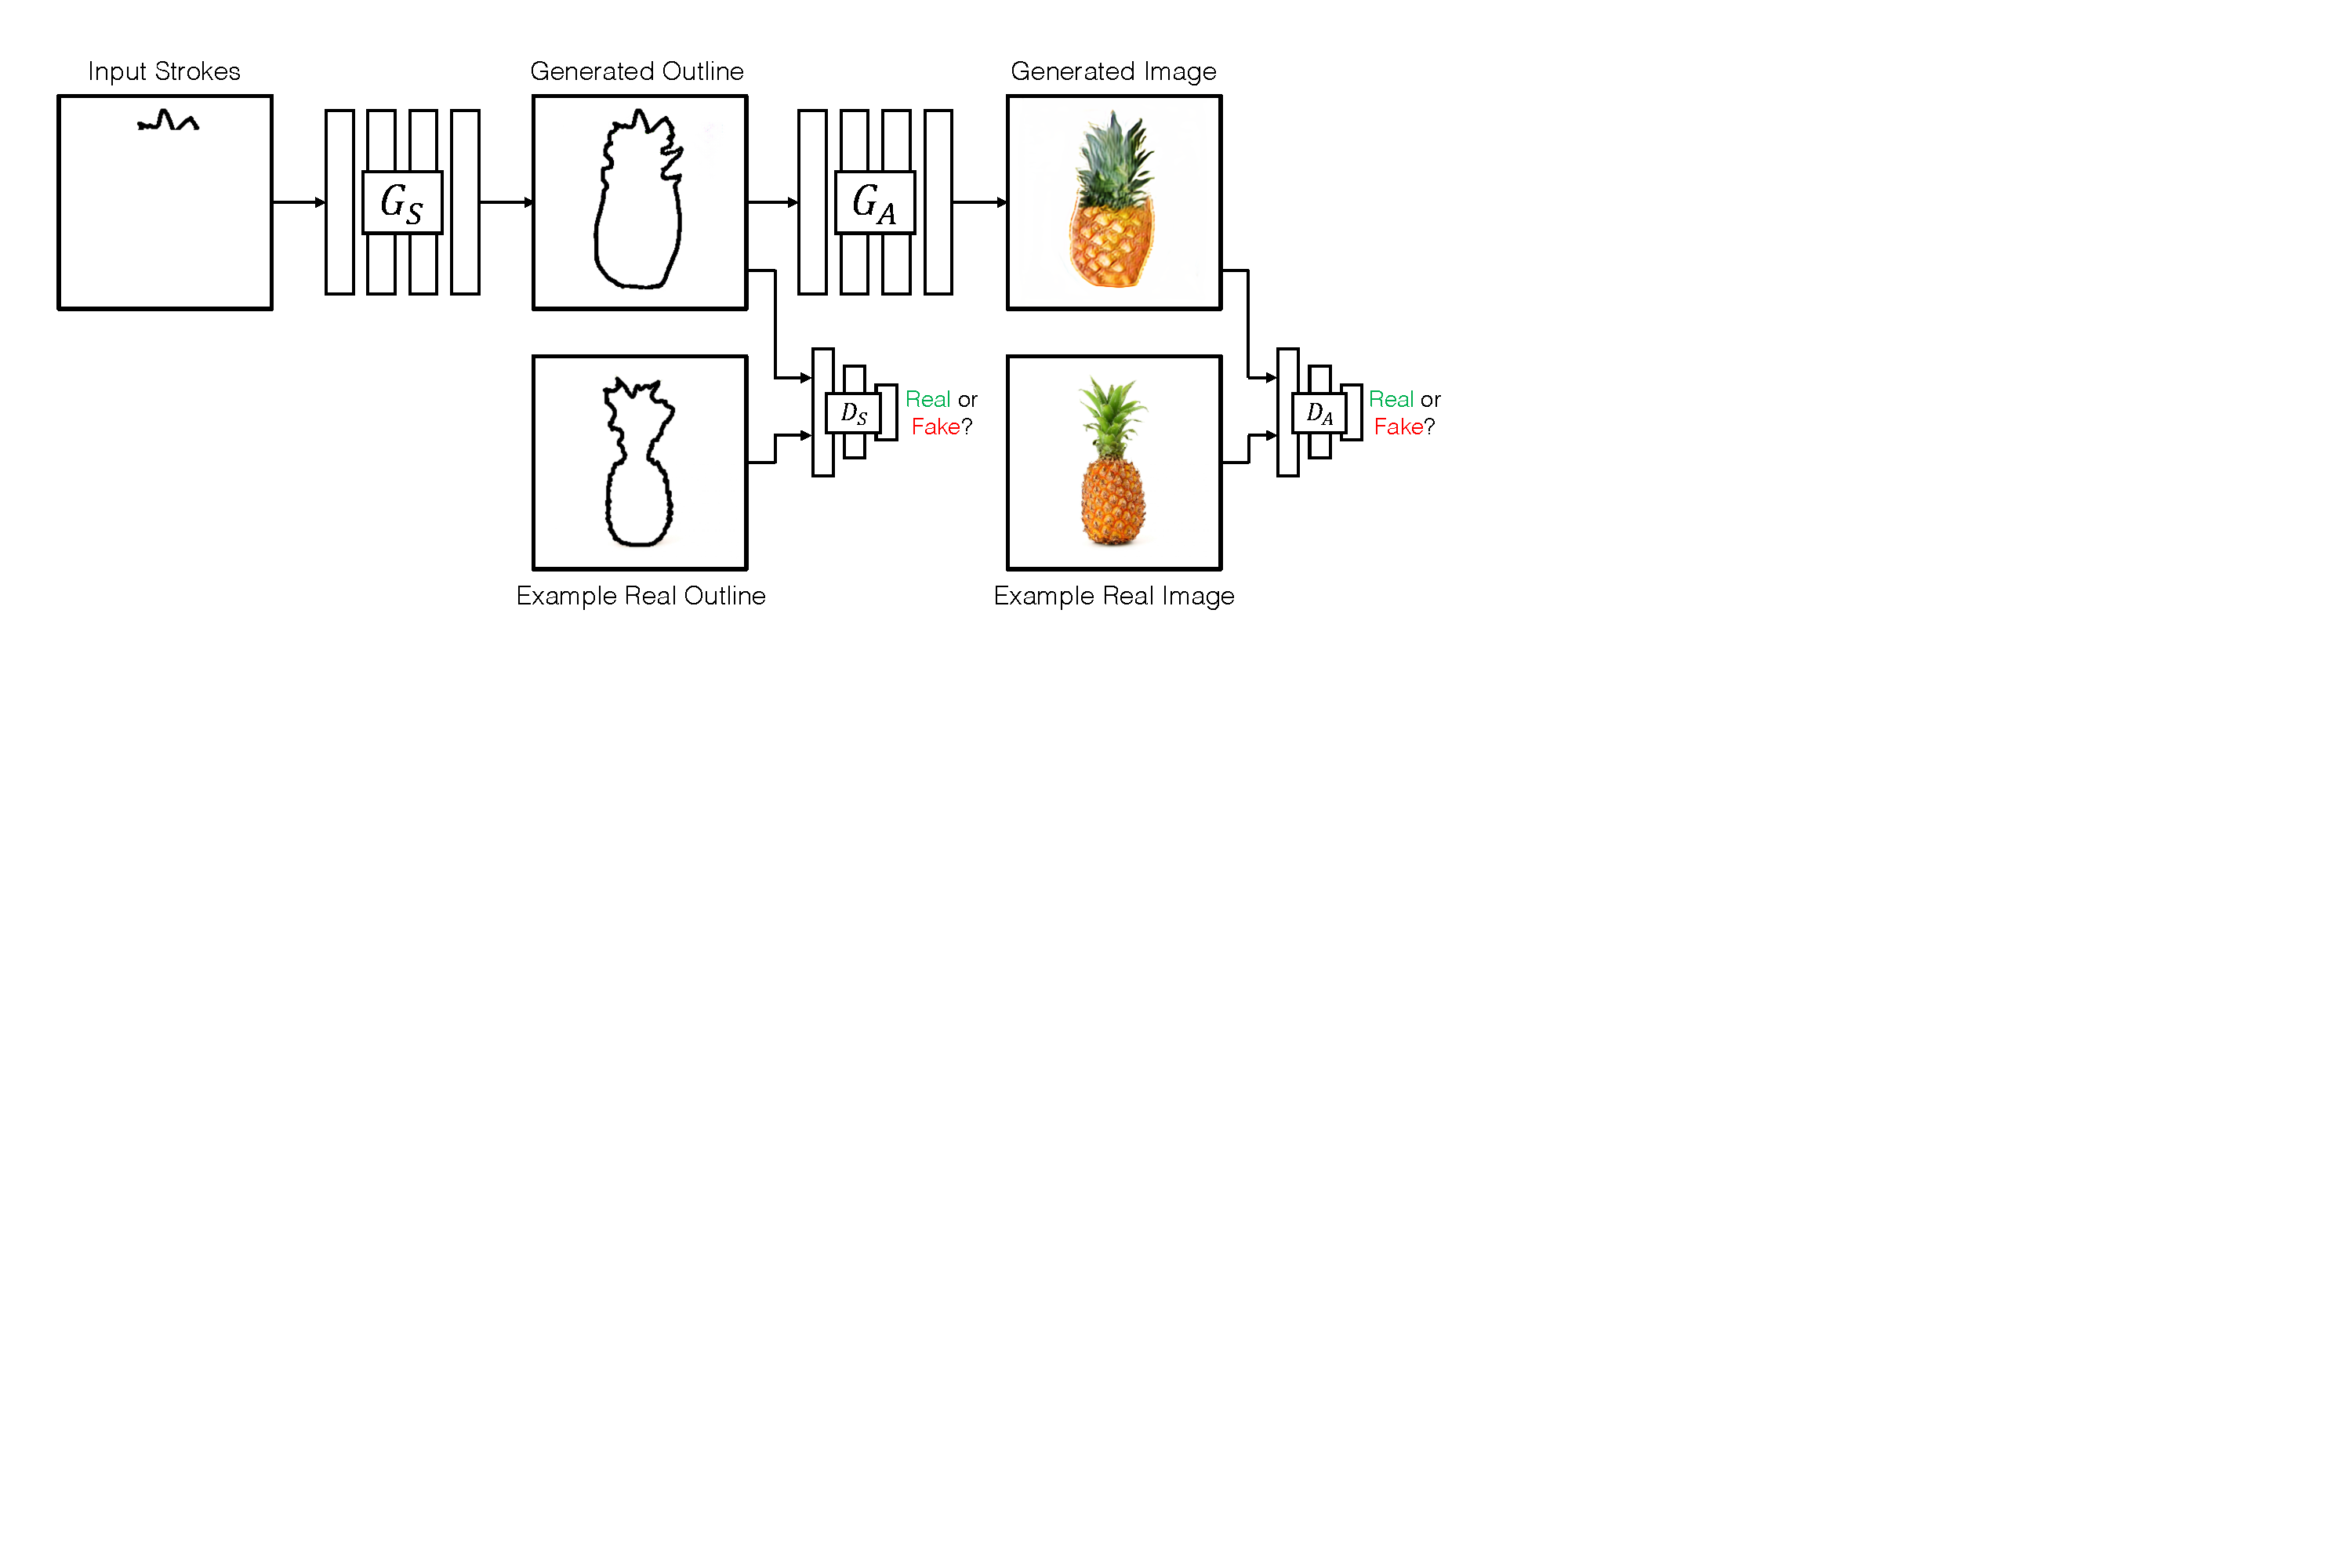
\includegraphics[width=.45\linewidth]{paper_images/isf_method_v3.pdf} &
		\includegraphics[width=.45\linewidth]{images/gif/00001.jpg} \hspace{4pt}
		\includegraphics[width=.45\linewidth]{images/gif_shadow/00001.jpg} 
		%\animategraphics[autoplay,loop,width=.45\linewidth]{25}{images/gif/}{00001}{00266} &
		%\animategraphics[autoplay,loop,width=.50\linewidth]{25}{images/gif_shadow/}{00001}{00096}
		\\
		% (a) & (b) \\
	\end{tabular}
	\caption{{\bf Video of our interface} We can see two versions of our interface. The left side shows how a user can quickly generate multiple objects using a few strokes, while the right side shows the utility of multimodal completions where the user can quickly explore different possible shape generations while drawing. Full video available at our \href{https://arnabgho.github.io/iSketchNFill/}{website}. { \textbf{Please view with Acrobat Reader.}}}\label{fig:gui}
	%\label{fig:gui}}
\end{figure}


\section{Related Work}

\paragraph{Interactive Generation} Interactive interfaces for freehand drawing go all the way back to Ivan Sutherland's Sketchpad~\cite{sutherland64}.  The pre-deep work most related to us, ShadowDraw~\cite{lee2011shadowdraw}, introduced the concept of generating multiple shadows for novice users to be able to draw sketches. PhotoSketcher \cite{eitz2011photosketcher} introduces a retrieval based method for obtaining real images from sketches. %Hays et al.~\cite{hays2007scene} introduce a retrieval-based method for filling scenes.
% \es{other old papers? Talk about ShadowDraw and other non-deep methods}. 
More recently, deep recurrent networks have been used to generate sketches~\cite{ha2017neural,ganin2018synthesizing}. Sketch-RNN~\cite{ha2017neural} provides a completion of partial strokes, with the advantage of intermediate stroke information via the Quickdraw dataset at training time. SPIRAL \cite{ganin2018synthesizing} learns to generate digits and faces using a reinforcement learning approach.
% to generate programs for synthesizing the final image.
Zhu et al.~\cite{zhu2016generative} train a generative model, and an optimization-based interface to generate possible images, given color or edge constraints. The technique is limited to a single class and does not propose a recommendation for the completion of the shape. SketchyGAN~\cite{chen2018sketchygan} also aimed at generating multi-class images but lacks interactive capability. In contrast to the above, our method provides interactive prediction of the shape and appearance to the user and supports multiple object classes.
% \vspace{-6mm}
\paragraph{Generative Modeling} Parametric modeling of an image distribution is a challenging problem. Classic approaches include autoencoders~\cite{hinton2006reducing,vincent2008extracting} and Boltzmann machines~\cite{smolensky1986information}. More modern approaches include autoregressive models~\cite{efros1999texture,van2016conditional}, variational autoencoders (VAEs)~\cite{kingma2013auto}, and generative adversarial networks (GANs). GANs and VAEs both learn mappings from a low-dimensional ``latent" code, sampled stochastically, to a high-dimensional image through a feedforward pass of a network. GANs have been successful recently~\cite{denton2015deep,radford2015unsupervised,arjovsky2017wgan}, and hybrid models feature both a learned mapping from image to latent space as well as adversarial training~\cite{donahue2016adversarial,dumoulin2016adversarially,larsen2016vaegan,chen2016infogan}.

% \vspace{2mm} 
\paragraph{Conditioned Image Generation} The methods described above can be conditioned, either by a low-dimensional vector (such as an object class, or noise vector), a high-dimensional image, or both. Isola et al.~\cite{isola2016image2image} propose ``pix2pix", establishing the general usefulness of conditional GANs for image-to-image translation tasks. However, they discover that obtaining multimodality by injecting a random noise vector is difficult, a result corroborated in~\cite{mathieu2015deep,pathak2016context,zhu2017toward}.
% introduced a set of tasks whereby the pixels of the input in a different domain corresponded to the pixels of the generated image.
% As a result, image-to-image translation methods have exploded in popularity, as many applications can be expressed in this framework.
% However, one problem with the original Pix2pix formulation is that the quality degrades quickly with increased class diversity. 
% We build upon these ideas by proposing a new architecture and gating scheme that allows for high quality multiclass image generation. 
% \paragraph{Mode Collapse}
This is an example of mode collapse~\cite{goodfellow2016nips}, a phenomenon especially prevalent in image-to-image GANs, as the generator tends or ignore the low-dimensional latent code in favor of the high-dimensional image.
% This is an example of mode collapse is a major challenge for GANs~\cite{goodfellow2016nips}, where the diversity of the generated results is limited and only a portion of the training set is utilized. 
Proposed solutions include layers which better condition the optimization, such as Spectral Normalization~\cite{zhang2018self,miyato2018spectral}, modifications to the loss function, such as WGAN~\cite{arjovsky2017wasserstein,gulrajani2017improved} or optimization procedure~\cite{heusel2017gans}, or modeling proposals, such as MAD-GAN~\cite{ghosh2017multi} and MUNIT~\cite{huang2018multimodal}. 
% Several techniques deal with this issue, the best performing among those include Spectral Normalization \cite{zhang2018self,miyato2018spectral} which normalizes the spectral norms of the layers to stabilize training, MAD-GAN \cite{ghosh2017multi} which introduces multiple generators, BicycleGAN \cite{zhu2017toward} which reconstructs the latent code from the generation using two cycles, and MUNIT \cite{huang2018multimodal} which introduces a factorized latent space for content and style for producing variations.
One modeling approach is to add a predictor from the output to the conditioner, to discourage the model from ignoring the conditioner. This has been explored in the classification setting in Auxiliary-Classifier GAN (ACGAN)~\cite{odena2016conditional} and regression setting with InfoGAN~\cite{chen2016infogan} and ALI/BiGAN (``latent regressor" model)~\cite{dumoulin2016adversarially,donahue2016adversarial}, and is one half of BicycleGAN model~\cite{zhu2017toward}. We explore a complementary approach of architectural modification via gating.


\noindent \textbf{Gating Mechanisms}
%Residual Networks \cite{he2016deep} introduced a new set of architectures that enabled training of very deep networks.
Residual networks~\cite{he2016deep}, first introduced for image classification~\cite{krizhevsky2012imagenet}, have made extremely deep networks viable to train. Veit et al.~\cite{veit2016residual} find that the skip connection in the architecture enables test-time removal of blocks. Follow-up work~\cite{veit2018adaptive} builds in block removal during training time, with the goal of subsets of blocks specializing to different categories. Inspired by these results, we propose the use of gating for image generation and provide a systematic analysis of gating mechanisms.
% Prior work has demonstrated that in ResNets, some paths are more important for particular classes~\cite{veit2016residual}, and has used this to develop a hard gating mechanism~\cite{veit2018adaptive}.
% We provide a further analysis of gating mechanisms, in the context of GAN image generation, as opposed to image classification.

The adaptive instance normalization (AdaIn) layer has similarly been used in arbitrary style transfer~\cite{huang2017arbitrary} and image-to-image translation~\cite{huang2018multimodal}, and Feature-wise Linear Modulation (FiLM)~\cite{perez2017film}. Both methods scale and shift feature distributions, based on a high-dimensional conditioner, such as an image or natural language question. Gating also plays an important role in sequential models for natural language processing: LSTMs \cite{hochreiter1997long} and GRU \cite{cho2014learning}. Similarly, concurrent work \cite{karras2018style}, \cite{park2019semantic} use a AdaIN-style network to modulate the generator parameters.
% \es{Mention concurrent work? StyleGAN, Taesung's paper}


\begin{figure}[t]
	\centering  
	% \begin{tabular}{cc}
	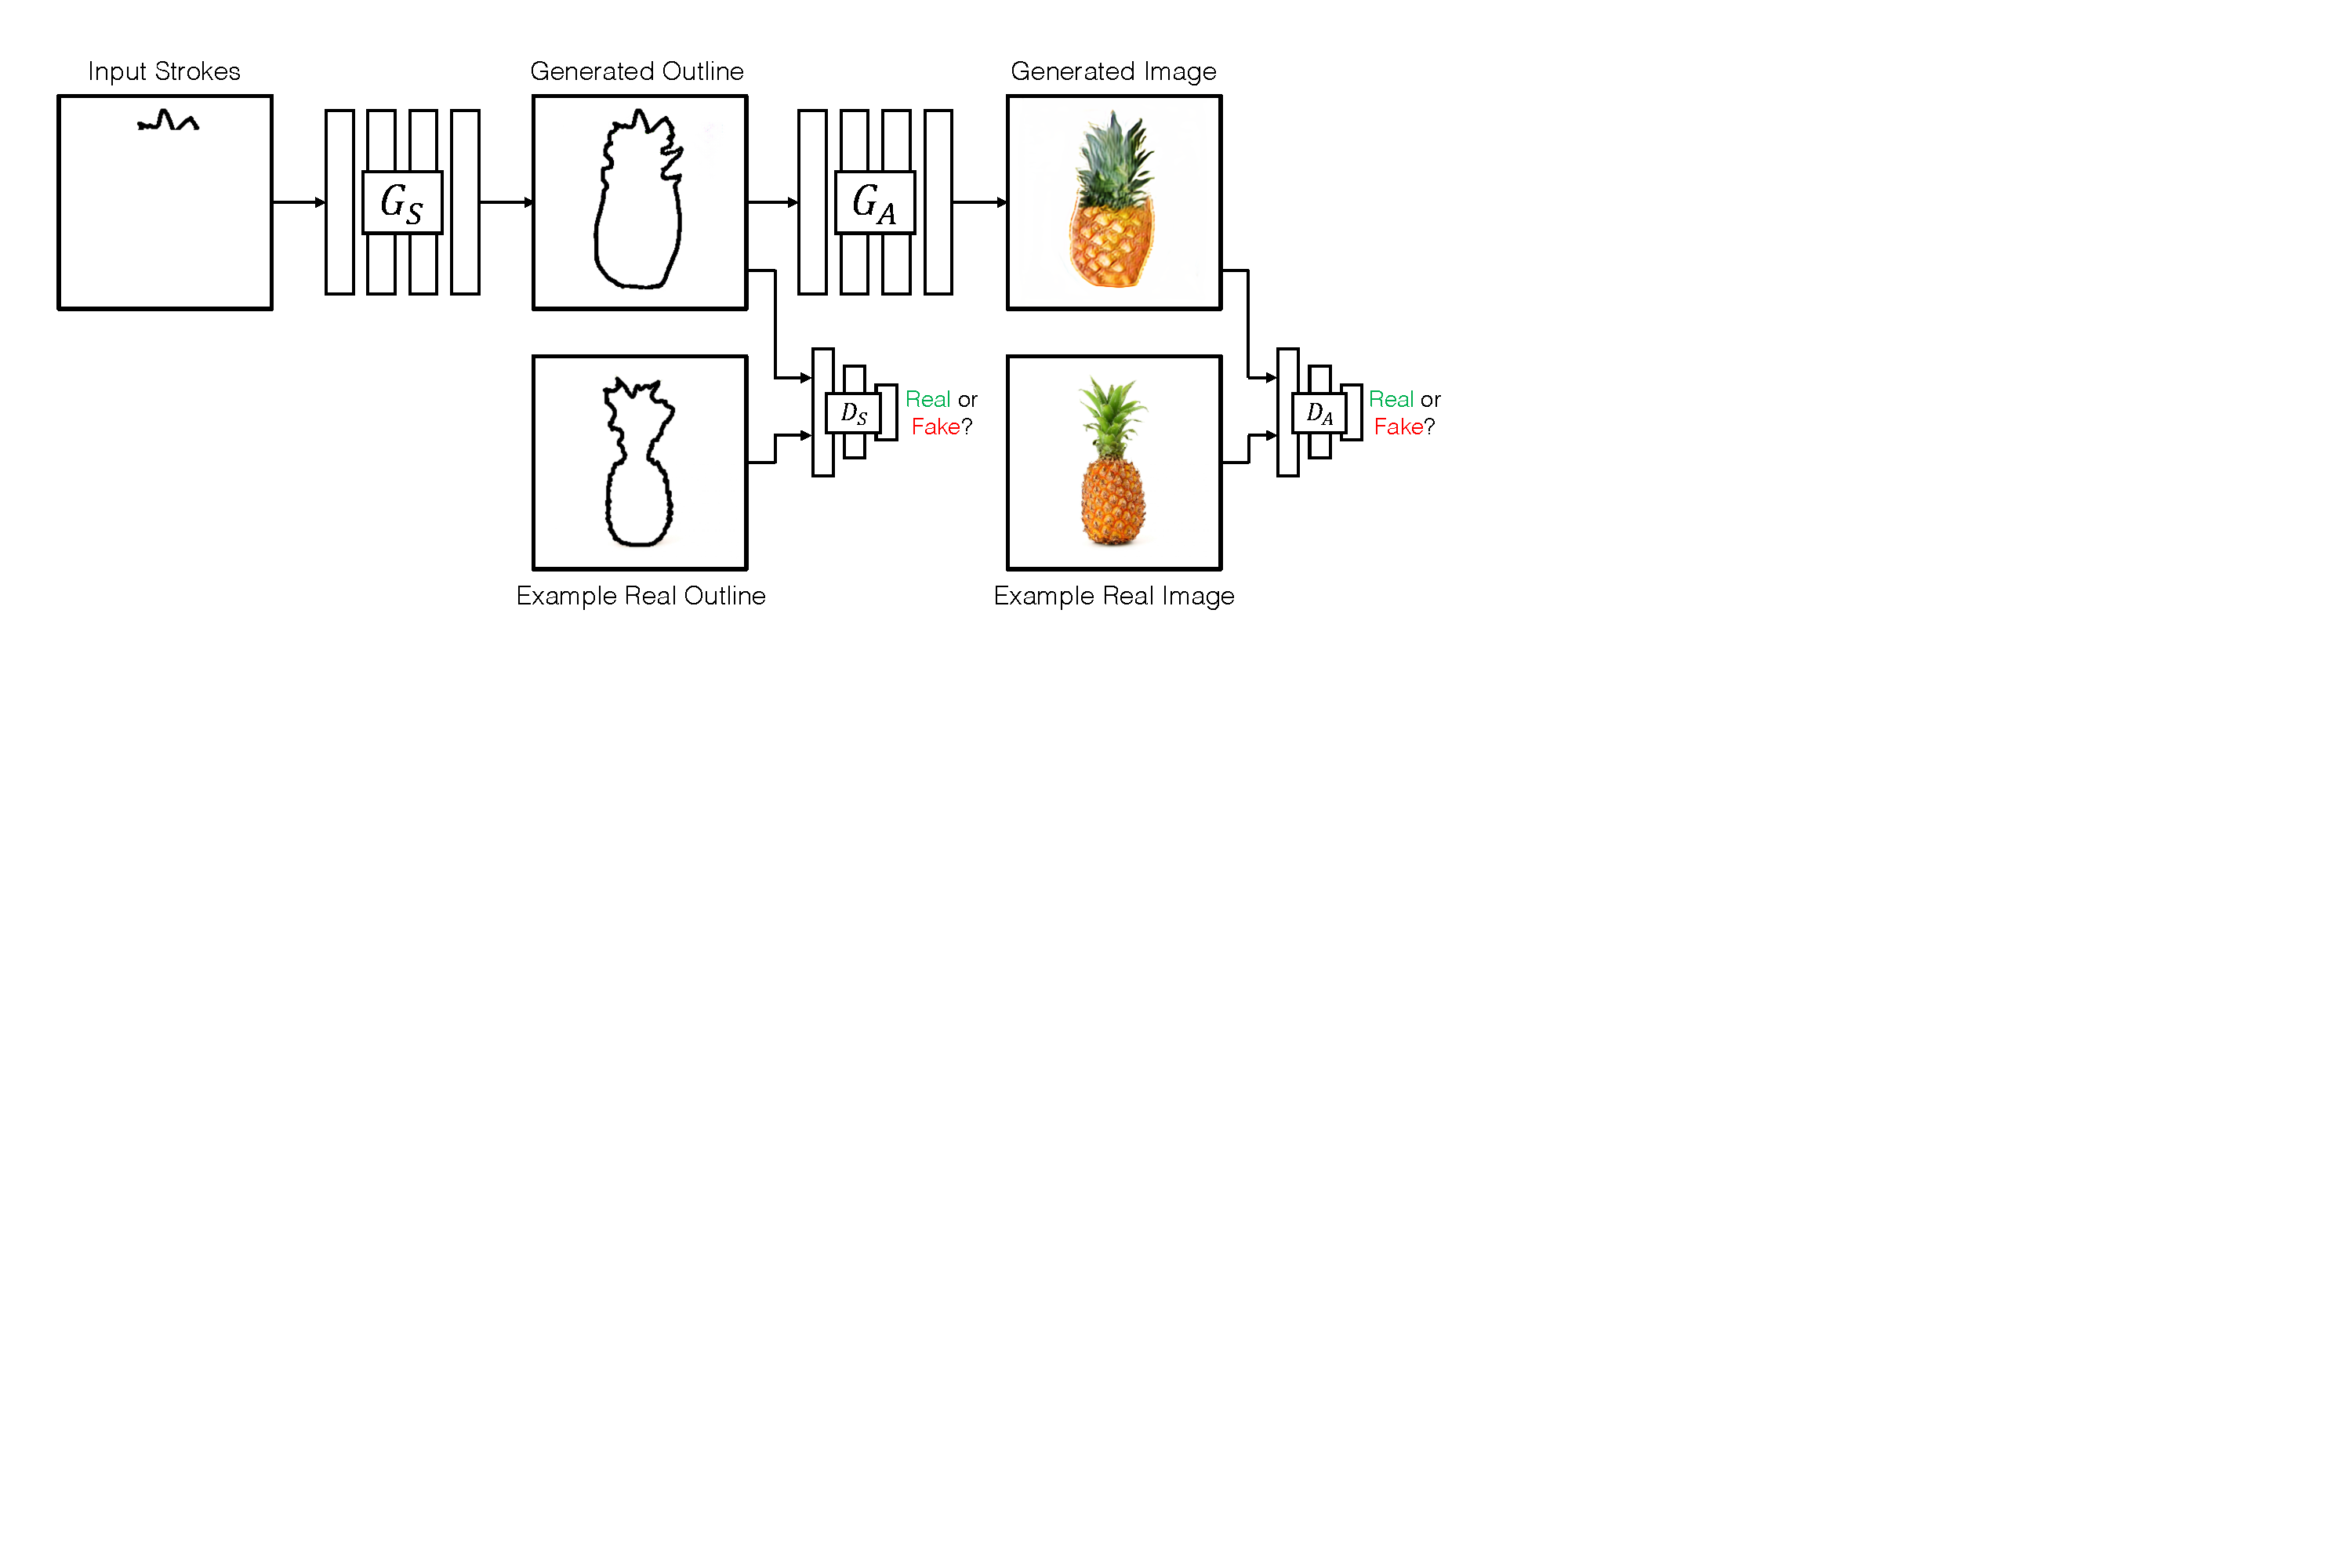
\includegraphics[width=\linewidth]{paper_images/isf_method_v3.pdf} 
	% 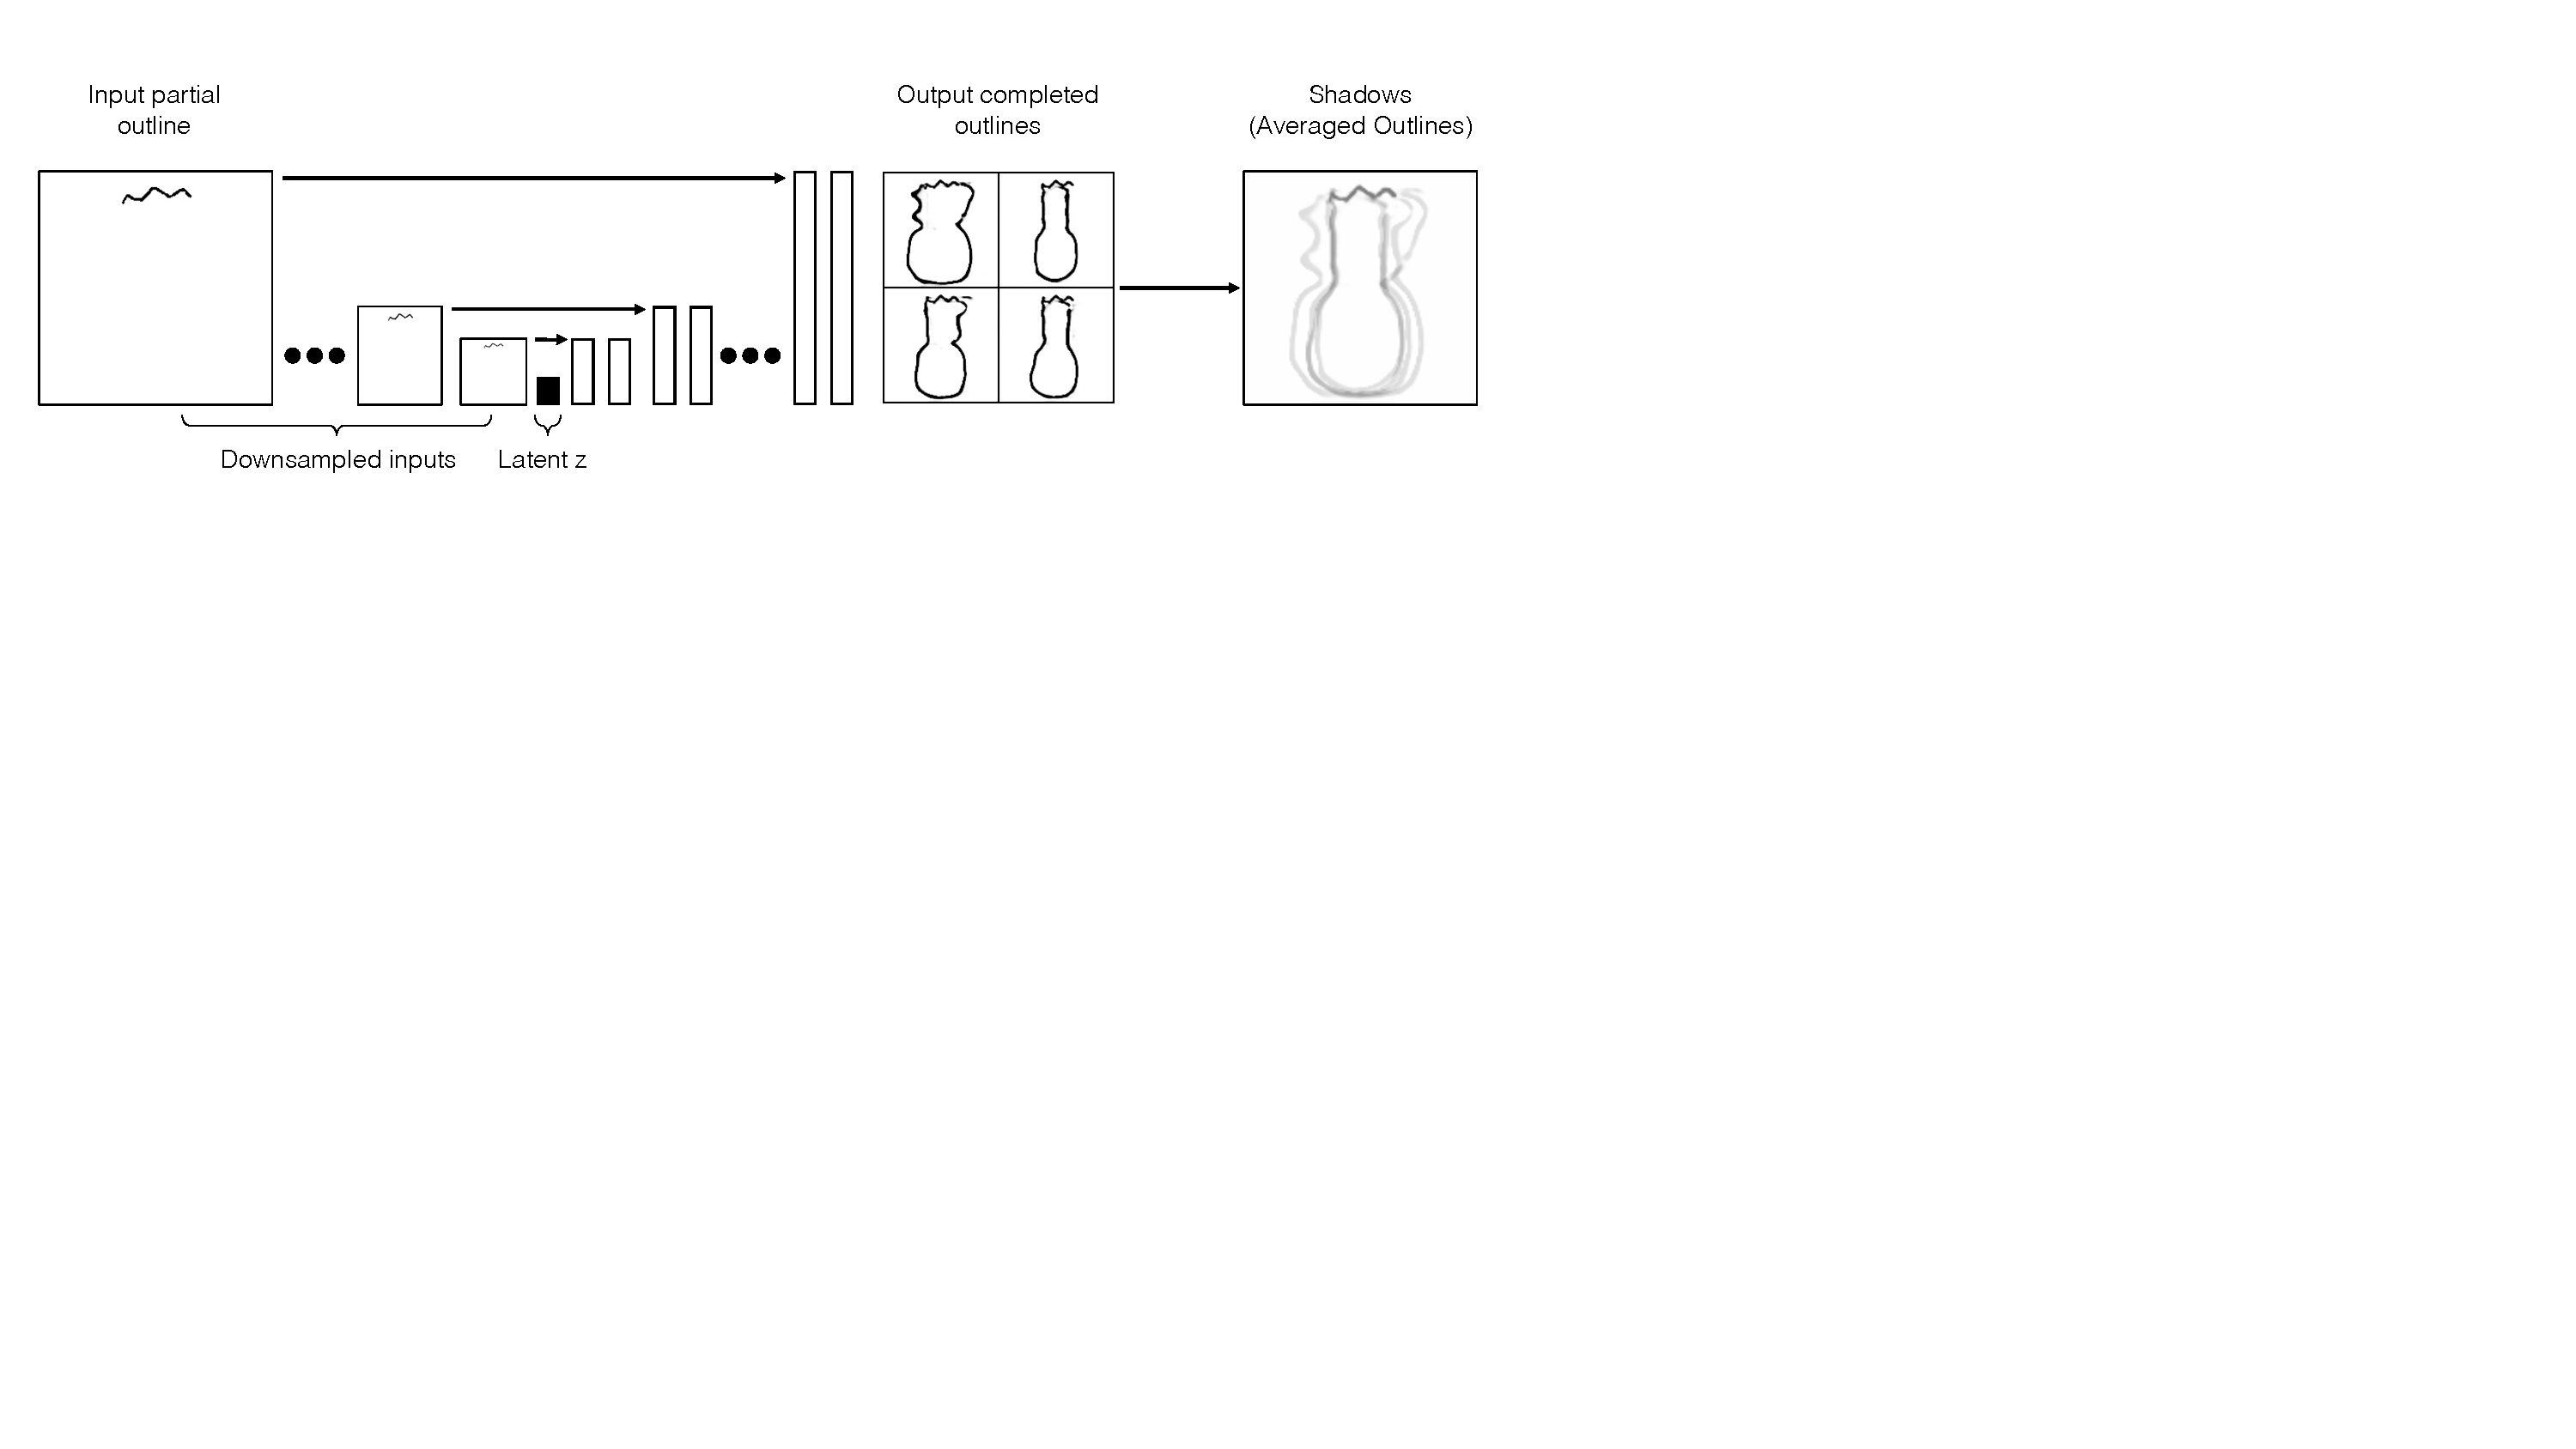
\includegraphics[width=.55\linewidth]{paper_images/shapegen.pdf}
	\\
	% (a) & (b) \\
	% \end{tabular}
	\vspace{-4mm}
	\caption{{\bf Our two-stage approach} First, we complete a partial sketch using the shape generator $G_S$. Then we translate the completed sketch into an image using the appearance generator $G_A$. Both generators are trained with their respective discriminators $D_S$, and $D_A$.
		{}}\label{fig:SketchFillNet}
	%\label{fig:gui}}
\end{figure}




\begin{figure*}[t]
	\centering
	% 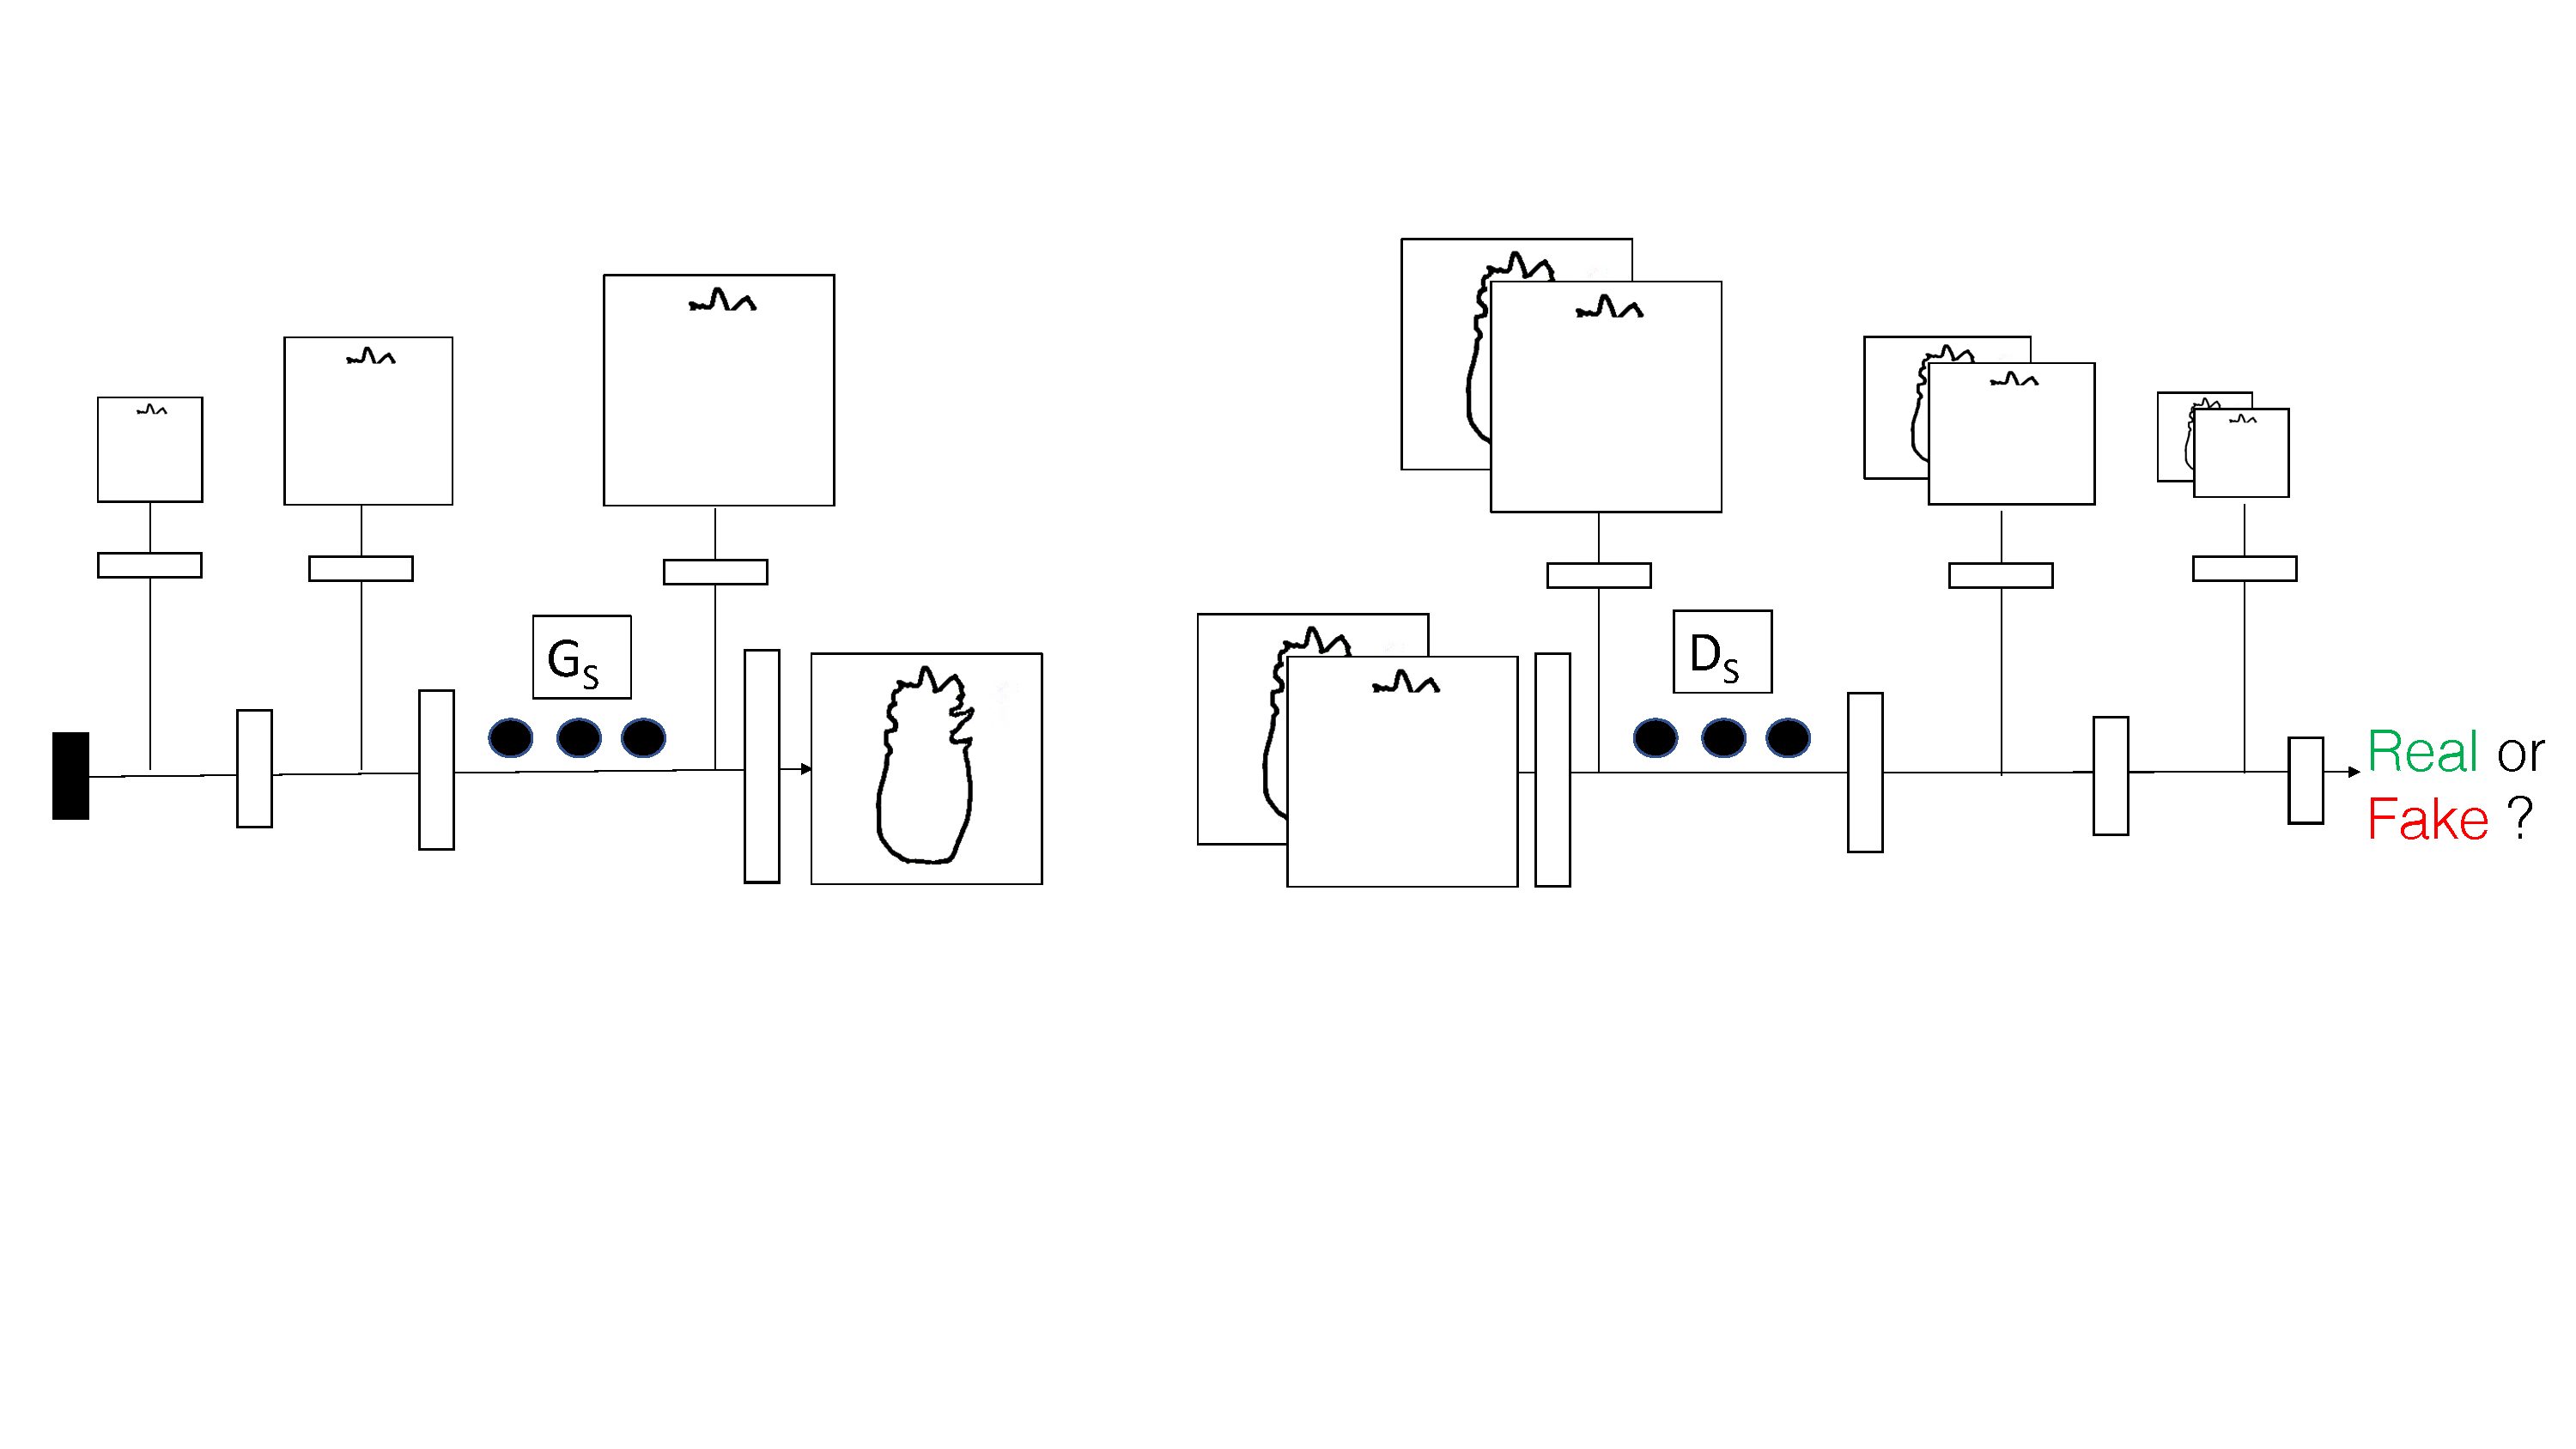
\includegraphics[width=\linewidth]{images/shape_completion/shape_completion.pdf}
	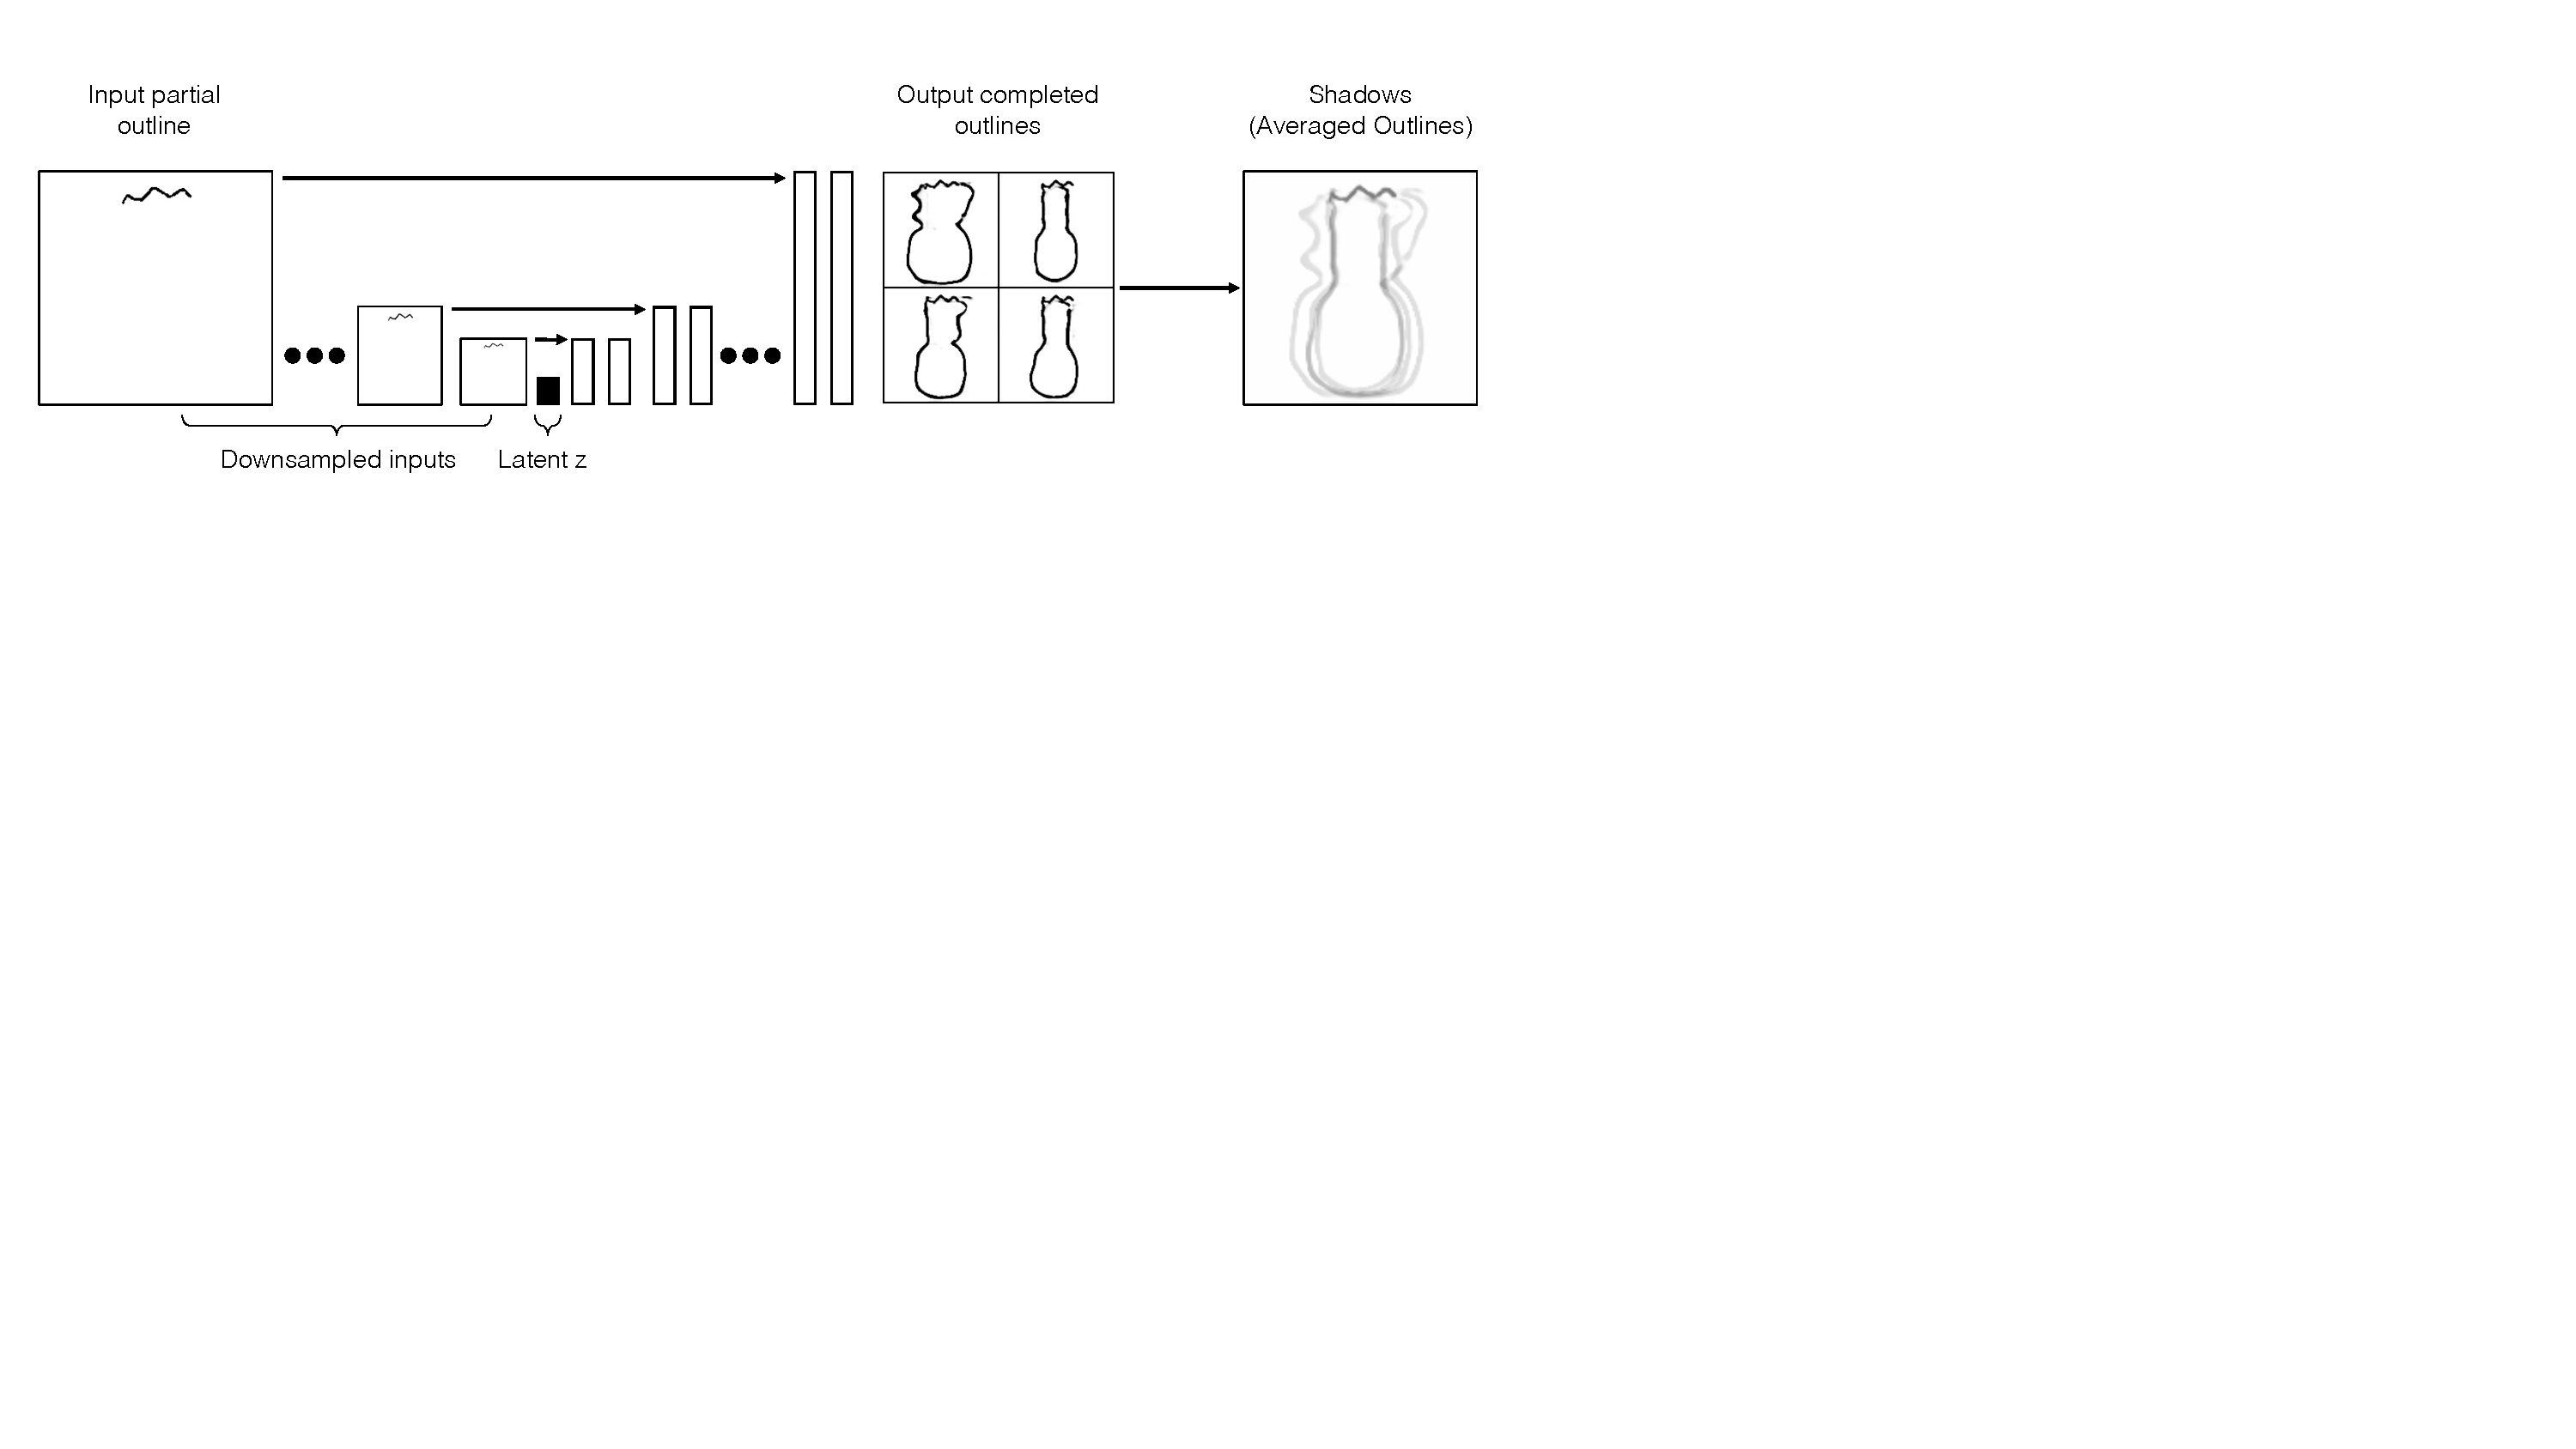
\includegraphics[width=\linewidth]{paper_images/shapegen.pdf}
	\vspace{-8mm}
	\caption{\textbf{First stage (Shape Generator)} To achieve multi-modal completions, the shape generator is designed using inspiration from non-image conditional model \cite{mescheder2018training} with the conditioning input provided at multiple scales, so that the generator network doesn't ignore the partial stroke conditioning.
		%$G_S$ design inspired from unconditional generator, with the conditioning provided at multiple scales to $G_S$ and $D_S$
	}\label{fig:SketchNet}
	%\vspace{-2mm}
\end{figure*}

\label{sec:methods}

\vspace{-4mm}
\section{Method}
We decouple the problem of interactive image generation into two stages: object shape completion from sparse user sketches, and appearance synthesis from the completed shape. More specifically, as illustrated in \figref{fig:SketchFillNet} we use the Shape Generator $G_S$ for the automatic shape (outline/sparse-sketch/simplified-edge) generation and the Appearance Generator $G_A$ for generating the final image as well as the adversary discriminators $D_S$ and $D_A$. Example usage is shown in our user interface in \figref{fig:gui}.

\subsection{Shape completion}
\label{sec:shape}
The shape completion network $G_S$ should provide the user with a visualization of its completed shape(s), based on the user input, and should keep on updating the suggested shape(s) interactively. 
%For an interactive user interface to be effective, the network has to generate an estimated full image shape as the user adds sparse input. 
We take a data-driven approach for this whereby, to train the network, we simulate partial strokes (or inputs) by removing random square patches from the full outline/ full sparse sketch/ full simplified edges. 
The patches are of three sizes (64$\times$64, 128$\times$128, 192$\times$192) and placed at a random location in the image of size 256$\times$256 (see \figref{fig:autocomplete_data_generation} for an example). To extend the technique beyond outlines and generate more human-like sketches, we adopt the multistage procedure depicted in \figref{fig:simplified_edges}. We refer to these generated sketches as ``simplified edges''.
% \es{probably need more details here - size of squares, how many per image, total training data size etc.}
We automatically generate data in this manner, creating a dataset where for a given full outline/sketch or a simplified edge-map, 75 different inputs are created.
%We found that the BicycleGAN model~\cite{zhu2017toward} performed well on the shape completion task, and we train it, unmodified, on pairs of partial-full outline images. %(Fig.~\ref{fig:infogan_gate}, top left).
The model, shown in \figref{fig:SketchFillNet}, is based on the architecture used for non-image conditional generations in \cite{mescheder2018training}. We modify the architecture such that the conditioning input is provided to the generator and discriminator at multiple scales as shown in \figref{fig:SketchNet}. This makes the conditioning input an active part of the generation process and helps in producing multimodal completions.


\begin{figure}[t]
	\centering
	\begin{tabular}{*{4}{c@{\hspace{3px}}}}
		\frame{
\includegraphics[width=.22\linewidth]{images/autocomplete_data_generation/original.png}} &
		\frame{
\includegraphics[width=.22\linewidth]{images/autocomplete_data_generation/64.png}} &
		\frame{
\includegraphics[width=.22\linewidth]{images/autocomplete_data_generation/128.png}} &
		\frame{
\includegraphics[width=.22\linewidth]{images/autocomplete_data_generation/192.png}}\\
		Outline &
		% 64$\times$64&
		% 128$\times$128 &
		% 192$\times$192
		\multicolumn{3}{c}{Simulated Partial Inputs}
		\\
	\end{tabular} \\
	\vspace{-3mm}
	\caption{\textbf{Simulated Inputs} Three sizes of occluders were used to simulate partial outlines.}
	\label{fig:autocomplete_data_generation}
\end{figure}

\begin{figure}[t]%[ht!]
	\centering
	\begin{tabular}{*{4}{c@{\hspace{3px}}}}
		\frame{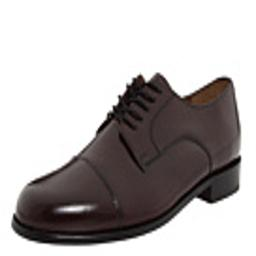
\includegraphics[width=.22\linewidth]{images/edge_simplification/1.jpg}} &
		\frame{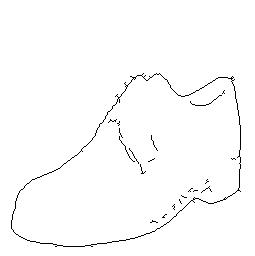
\includegraphics[width=.22\linewidth]{images/edge_simplification/1_edge.jpg}} &
		\frame{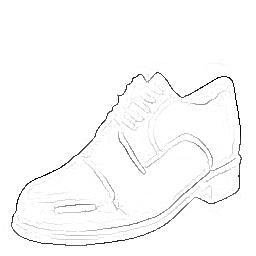
\includegraphics[width=.22\linewidth]{images/edge_simplification/1_edge_tone.jpg}} &
		\frame{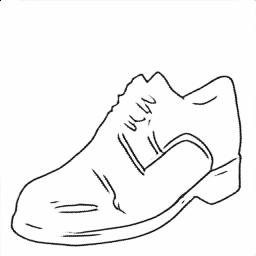
\includegraphics[width=.22\linewidth]{images/edge_simplification/1_simplified_edge.jpg}}
		\\
		
		% \begin{subfigure}[t]{.25\linewidth}\caption{}\label{fig:basketball_partial}\end{subfigure} &
		% \begin{subfigure}[t]{.25\linewidth}\caption{}\label{fig:basketball_full}\end{subfigure} &
		% \begin{subfigure}[t]{.25\linewidth}\caption{}\label{fig:basketball_full}\end{subfigure} &
		% \begin{subfigure}[t]{.25\linewidth}\caption{}\label{fig:soccer_partial}\end{subfigure} \\
	\end{tabular} \\
	\caption{\textbf{Simplified Edges} The 2nd edgemap is obtained using the technique of \cite{isola2016image2image}, while the 3rd is the intermediate edgemap using \cite{li2019im2pencil} and further simplified using \cite{simo2016learning} which looks closer to what a human would sketch. }
	\label{fig:simplified_edges}
	\vspace{-3mm}
\end{figure}

\vspace{-4mm}
\begin{figure*}[t]
	\centering
	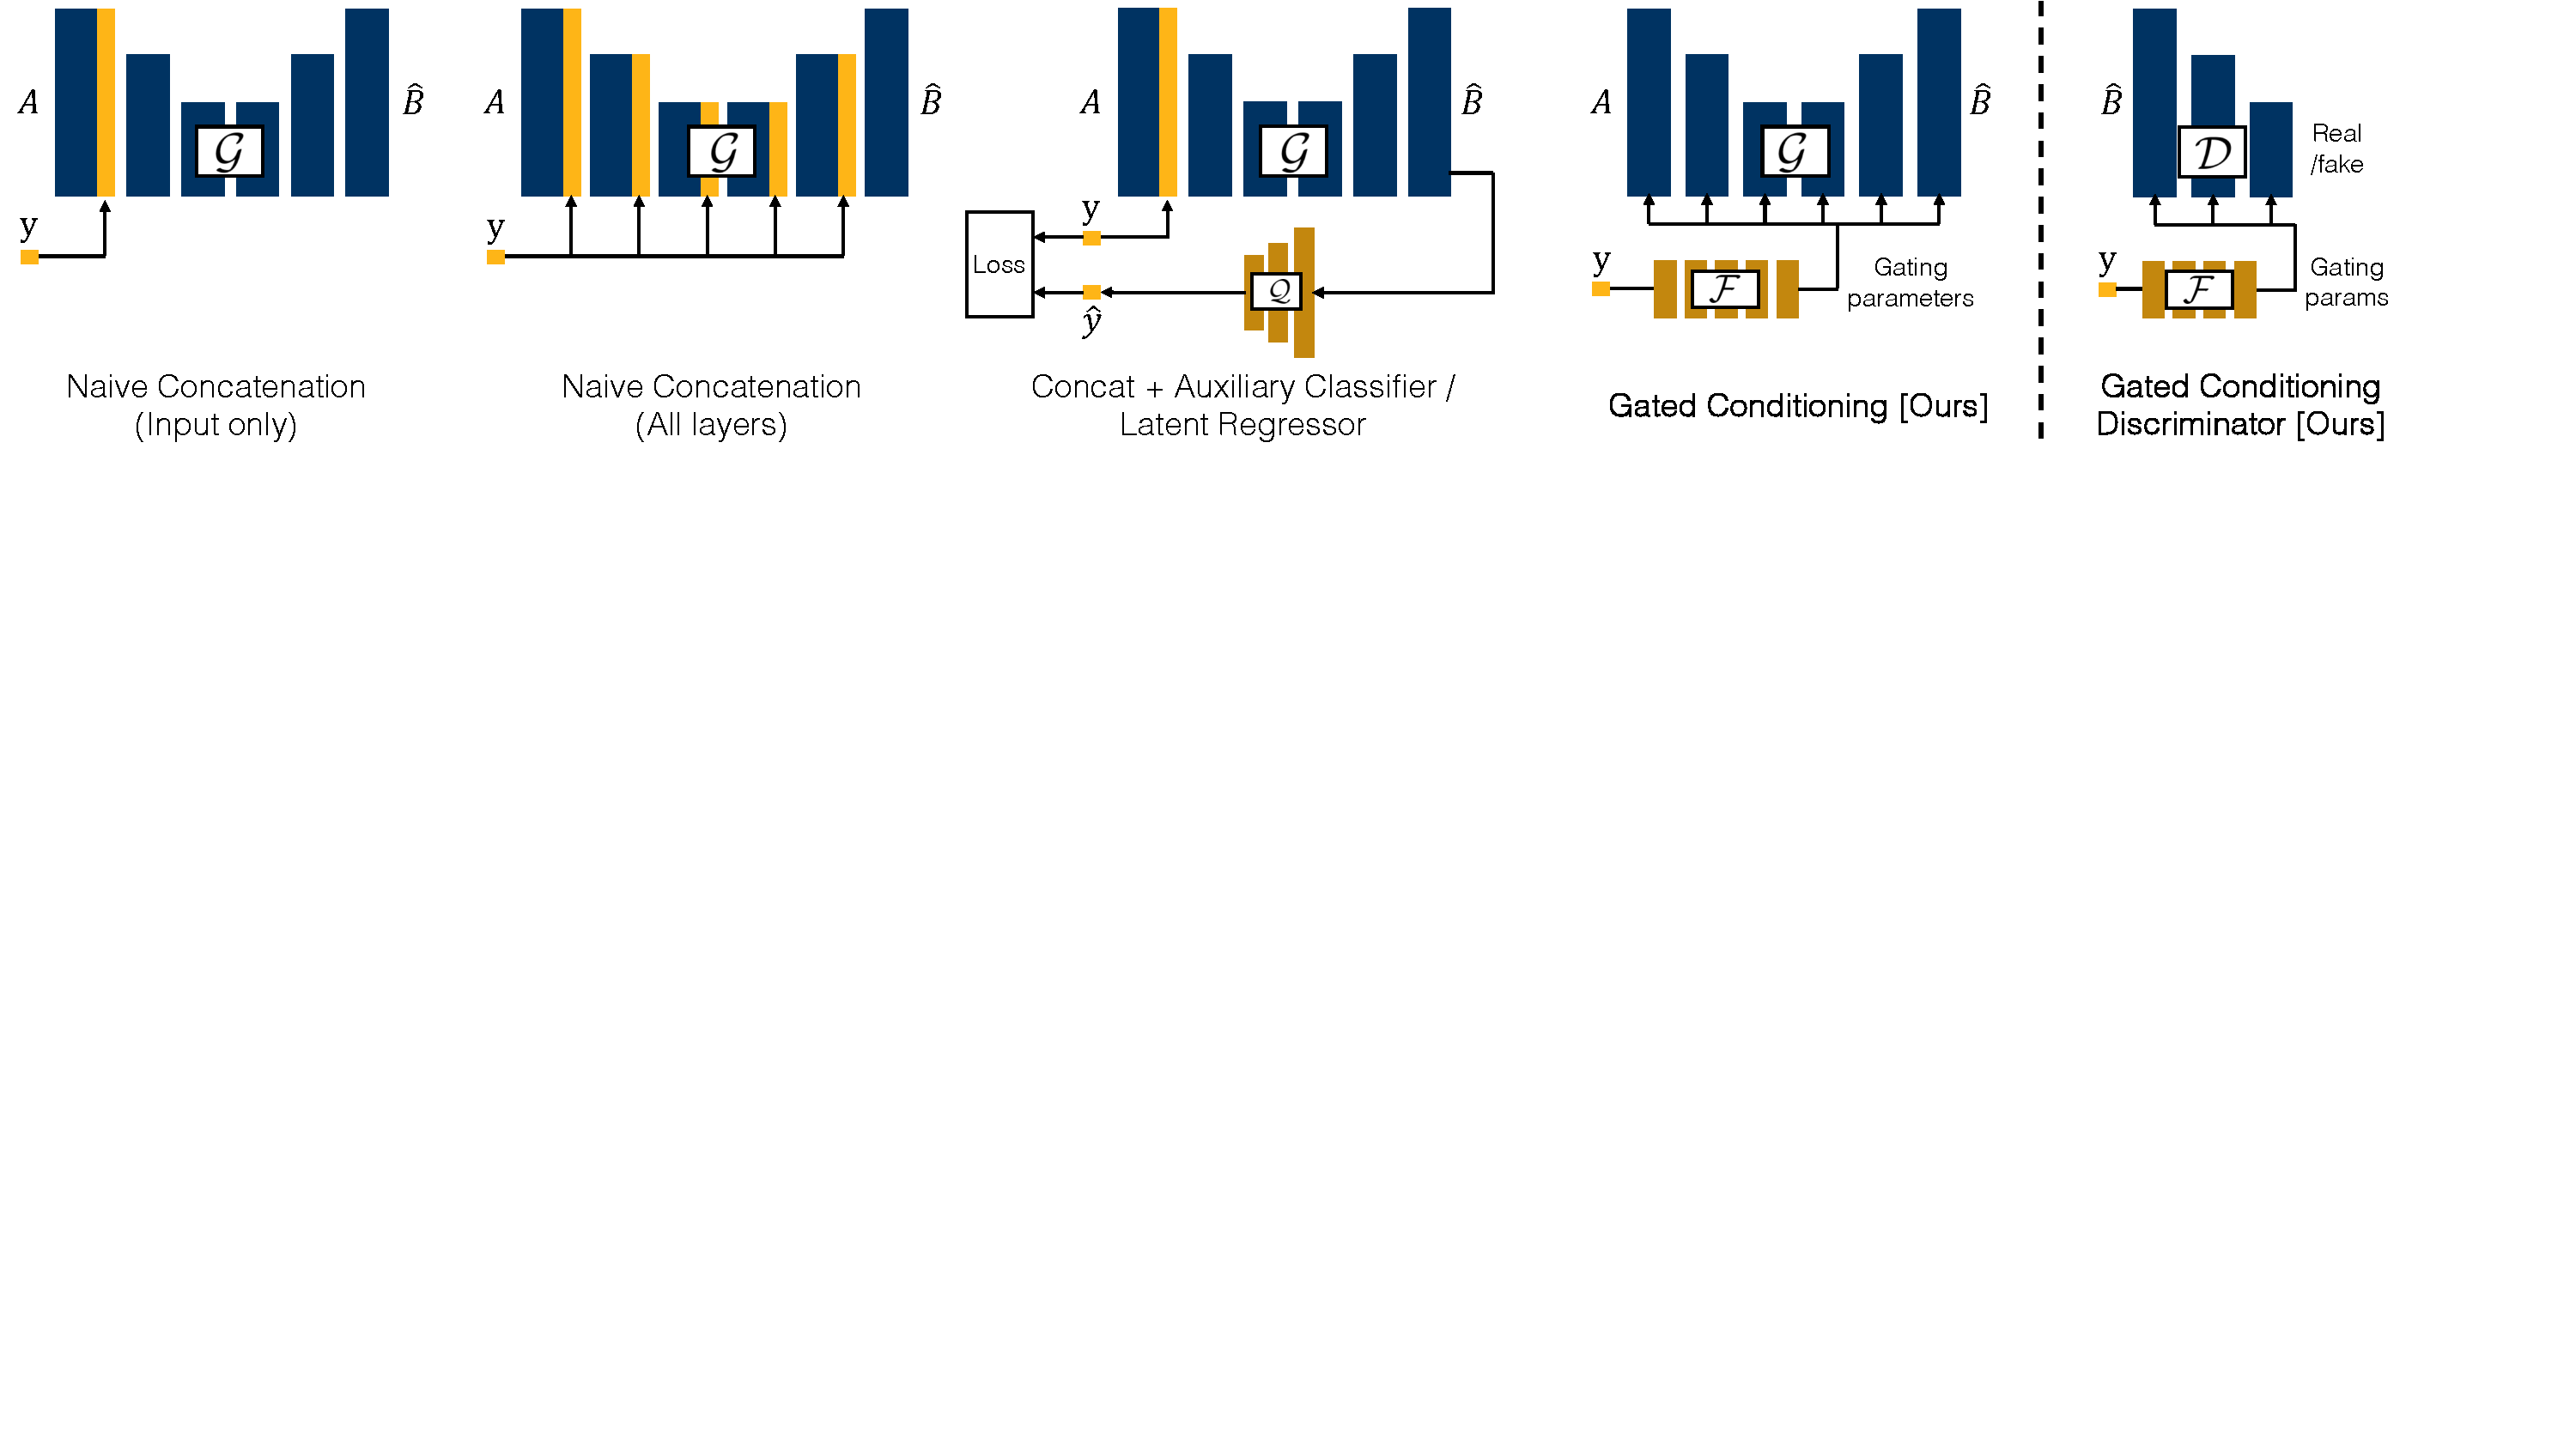
\includegraphics[width=1.\linewidth]{paper_images/arch_inject2.pdf}
	\vspace{-6mm}
	\caption{
		% \vspace{-2mm}
		{\bf Conditioning variants for the Appearance Generator} Our model uses gating on all the residual blocks of the generator and the discriminator, other forms of conditioning such as (naive concatenation in input only, all layers, AC-GAN like latent regressor \cite{odena2016conditional}) are evaluated as well. \label{fig:arch-gate1}
		% \vspace{-2mm}
	}
\end{figure*}

\begin{figure*}[t]
	\centering
	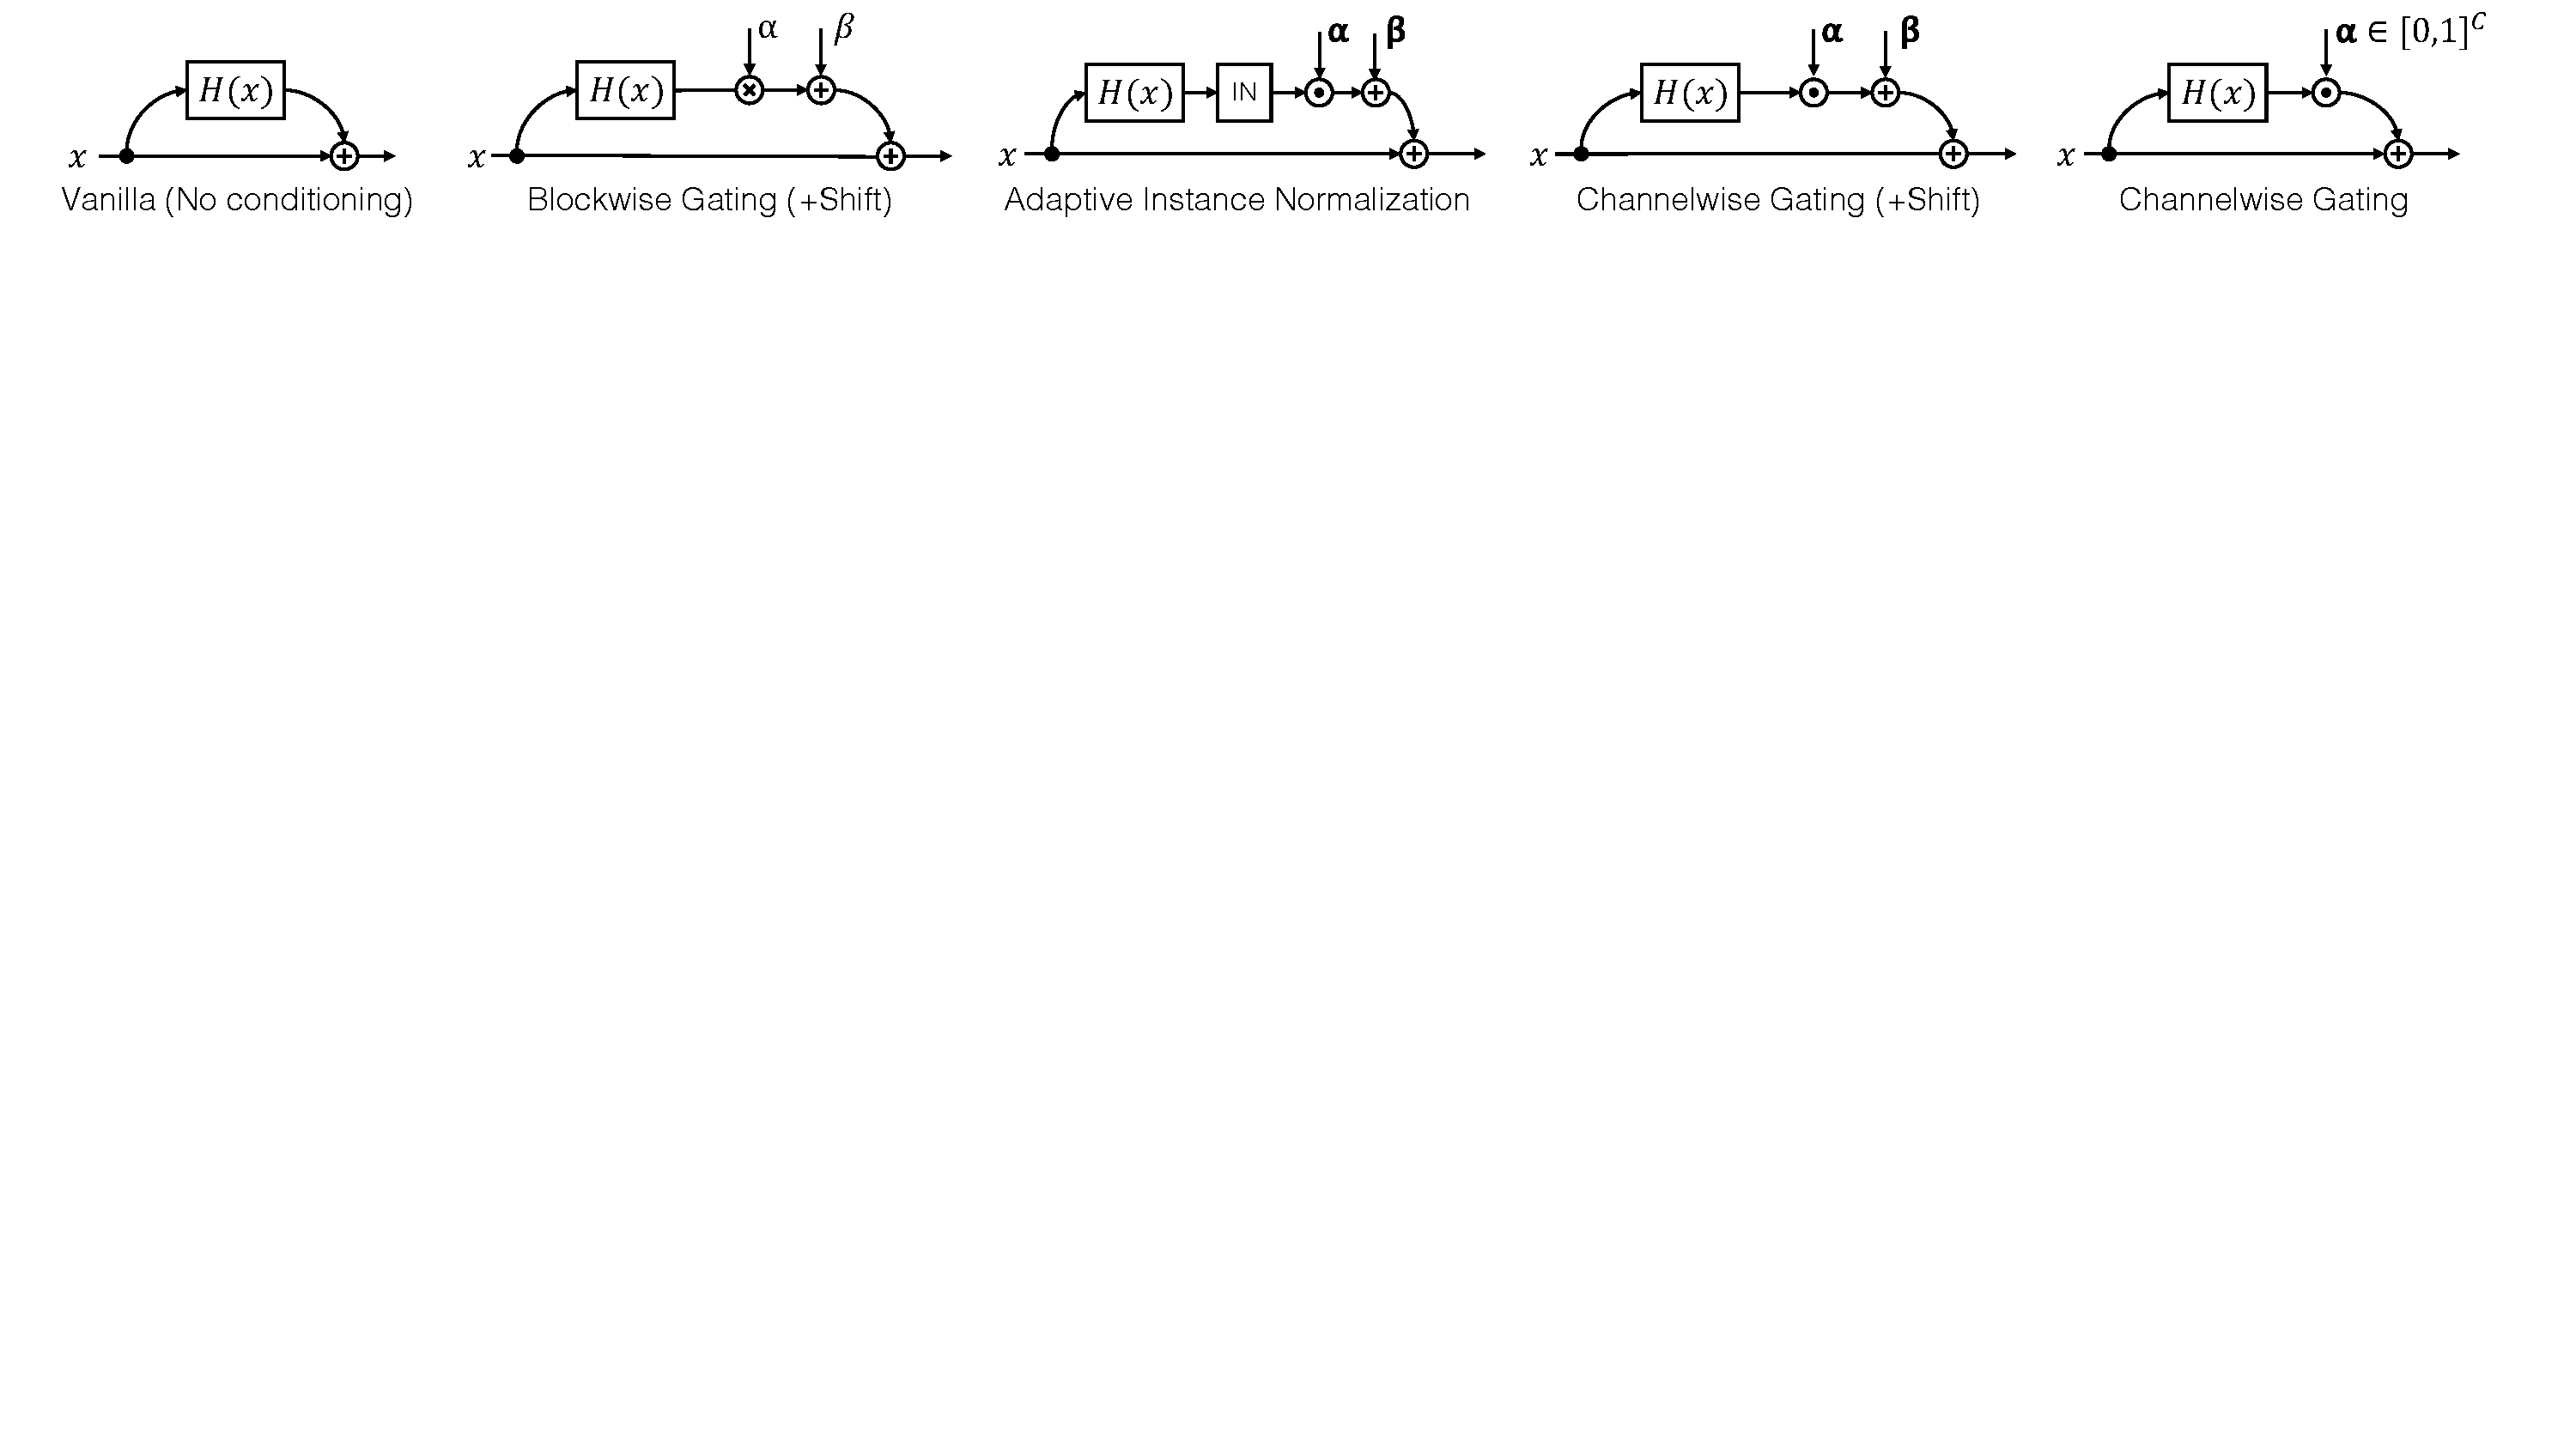
\includegraphics[width=1.\linewidth]{paper_images/arch_gate3.pdf}
	\vspace{-4mm}
	\caption{
		% {\bf Incorporating soft-gating into residual blocks.} \rz{Order got changed, may or may not need to add key for hadamard product}
		{\bf Injecting conditioning with modified residual layers} {\bf (Left)} A ``vanilla" residual block without conditioning applies a residual modification to the input tensor. {\bf (Mid-left)} The $\mathcal{H}(X)$ block is softly-gated by scalar parameter $\alpha$ and shift $\beta$. {\bf (Mid)} Adaptive Instance Normalization~\cite{huang2017arbitrary} applies a channel-wise scaling and shifting after an instance normalization layer. {\bf (Mid-right)} Channel-wise gating adds restrictions to the range of $\mbox{\boldmath $\alpha$}$. {\bf (Right)} We find that channel-wise gating (without added bias) produces the best results empirically.\label{fig:arch-gate2}
		\vspace{-2mm}
	}
\end{figure*}


\vspace{4mm}
\subsection{Appearance synthesis}
\label{sec:appearance}
%We use a conditional GAN formulation for generating images from outlines as shown by the efficacy in \cite{isola2016image2image,zhu2017toward}. 
An ideal interactive sketch-to-image system  should be able to generate multiple different image classes with a single generator. 
Beside memory and time considerations (avoiding loading/using a separate model per class, reducing overall memory), a single network can share features related to outline recognition and texture generation that are common across classes, which helps training with limited examples per class. %\es{Didn't we already said that in the intro? If yes we should remove/significantly shorten}

As we later show, class-conditioning by concatenation can fail to properly condition the network about the class information in current image translation networks~\cite{isola2016image2image,zhu2017toward}.
%
To address this, we propose an effective soft gating mechanism, shown in~\figref{fig:arch-gate1}.
Conceptually, our network consists of a small external gating network that is conditioned on the object class (encoded as a 1-hot vector).
The gating network outputs parameters that are used to modify the features of the main generator network.
Given an input feature tensor $X_l$, ``vanilla'' ResNet~\cite{he2016deep} maps it to
\begin{equation}
	X_{l+1} = X_l+\mathcal{H}_l(X_l).
\end{equation}
Changes in resolution are obtained by upsampling before or downsampling after the residual block.
Note that we omit $l$ subscript from this point forward to reduce clutter.
Our gating network augments this with a predicted scalar $\alpha$ for each layer of the network using a learned network $\mathcal{F}({\bf y})$, where ${\bf y}$ is the conditioning vector:
\begin{equation}
	X + \alpha \; \mathcal{H}(X), \text{where } \alpha \in [0,1]
\end{equation}

If the conditioning vector ${\bf y}$ has no use for a particular block, it can predict $\alpha$ close to zero and effectively switch off the layer.
% , and use that layer instead for other classes.
During training, blocks within the main network can transform the image in various ways, and $\mathcal{F}$ can modulate such that the most useful blocks are selected. 
Unlike previous feature map conditioning methods such as AdaIn~\cite{ulyanovinstance}, we apply gating to \emph{both} the generator and discriminator. 
This enables the discriminator to select blocks which effectively judge whether generations are real or fake, conditioned on the class input.
% Via accurate gradients backpropagated to the generator it also enables the generator to generate class conditioned high resolution image samples.
Some blocks can be shared across regions in the conditioning vector, whereas other blocks can specialize for a given class.

A more powerful method is to apply this weighting channel-wise using a vector {\boldmath$\alpha$}: % This is denoted as follows:
\begin{align}
	X + \mbox{\boldmath $\alpha$} \odot \mathcal{H}(X), \text{where } \mbox{\boldmath $\alpha$} \in [0,1]^c, 
\end{align}
where $\odot$ represents channel-wise multiplication. This allows specific channels to be switched ``on" or ``off", providing additional degrees of freedom.
%We make the corresponding changes in the discriminator as well. 
%Soft-gating has been explored by Veit et al.~\cite{veit2018adaptive} in a classification setting. 
We found that this channelwise approach for gating provides the strongest results. 
AdaIn describes the case where an Instance Normalization~\cite{ulyanovinstance} (IN) operation is applied before scaling and shifting the feature distribution.
We constrain each element of {\boldmath $\alpha$} and {\boldmath $\beta$} in $[-1, 1]$.
We additionally explored incorporating a bias term after the soft-gating, either block-wise using a scalar $\beta \in [-1,1]$ per layer, or channel-wise using a vector $\mbox{\boldmath $\beta$} \in [-1, 1]^c$ per layer but we found that they did not help much, and so we leave them out of our final model. Refer \figref{fig:arch-gate2} for pictorial representation of various gatings.
% \ow{but found that they did not help much, and so we leave them out of our final model?}


Finally, we describe our network architecture, which utilizes the gated residual blocks described above.
We base our architecture on the proposed residual \textbf{Encoder-Decoder} model from MUNIT~\cite{huang2018multimodal}.
This architecture is comprised of 3 \texttt{conv} layers, 8 residual blocks, and 3 \texttt{up-conv} layers. The residual blocks have 256 channels. 
First, we deepen the network, based on the principle that deeper networks have more valid disjoint, partially shared paths~\cite{veit2016residual}, and add 24 residual blocks. 
To enable the larger number of residual blocks, we drastically reduce the width to 32 channels for every layer. 
We refer to this network as \textbf{SkinnyResNet}. 
Additionally, we found that modifying the downsampling and upsampling blocks to be residual connections as well improved results, and also enables us to apply gating to {\em all} blocks. 
When gating is used, the gate prediction network, $\mathcal{F} ({\bf y})$,  
%Fig.~\ref{fig:arch-inj} (mid-right, right) 
is also designed using residual blocks. Additional architecture details are in the supplementary material. 


\begin{figure*}[t]
	\begin{tabular}{cc}
		\resizebox{0.5\linewidth}{!}{
			\begin{tabular}{*{5}{c@{\hspace{3px}}}}
				\frame{
\includegraphics[width=.12\linewidth]{images/shoe_autocomplete_render/current_scribble_5.jpg}} &
				%\frame{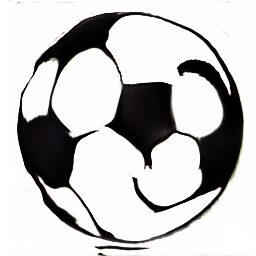
\includegraphics[width=.10\linewidth]{images/autocomplete_generate/scribble/soccer.png}} &
				\frame{
\includegraphics[width=.12\linewidth]{images/shoe_autocomplete_render/current_scribble_6.jpg}} & 
				\frame{
\includegraphics[width=.12\linewidth]{images/shoe_autocomplete_render/current_scribble_7.jpg}}&
				\frame{
\includegraphics[width=.12\linewidth]{images/shoe_autocomplete_render/current_scribble_8.jpg}} &
				\\
				\frame{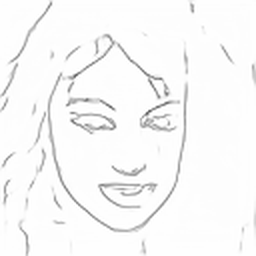
\includegraphics[width=.12\linewidth]{images/shoe_autocomplete_render/autocompleted_sketch_5.png}} &
				%\frame{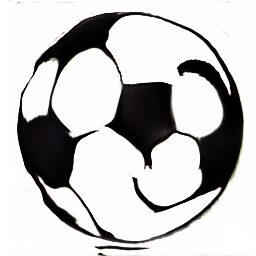
\includegraphics[width=.10\linewidth]{images/autocomplete_generate/scribble/soccer.png}} &
				\frame{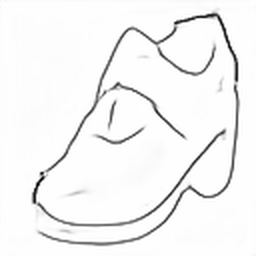
\includegraphics[width=.12\linewidth]{images/shoe_autocomplete_render/autocompleted_sketch_6.png}} & 
				\frame{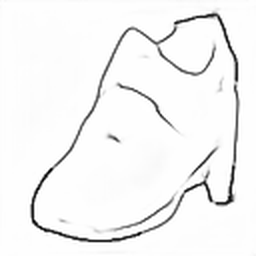
\includegraphics[width=.12\linewidth]{images/shoe_autocomplete_render/autocompleted_sketch_7.png}}&
				\frame{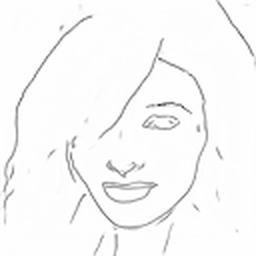
\includegraphics[width=.12\linewidth]{images/shoe_autocomplete_render/autocompleted_sketch_8.png}} &
				
				\\
				\frame{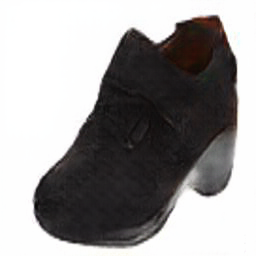
\includegraphics[width=.12\linewidth]{images/shoe_autocomplete_render/rendered_5.png}} &
				%\frame{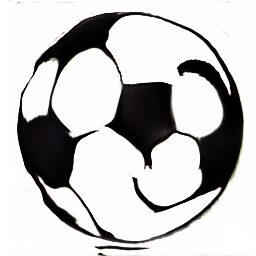
\includegraphics[width=.10\linewidth]{images/autocomplete_generate/scribble/soccer.png}} &
				\frame{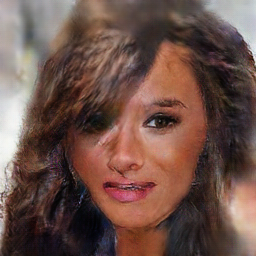
\includegraphics[width=.12\linewidth]{images/shoe_autocomplete_render/rendered_6.png}} & 
				\frame{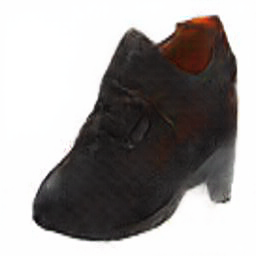
\includegraphics[width=.12\linewidth]{images/shoe_autocomplete_render/rendered_7.png}}&
				\frame{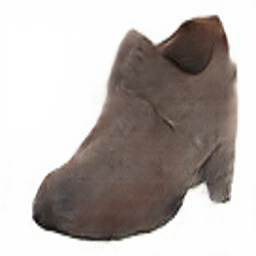
\includegraphics[width=.12\linewidth]{images/shoe_autocomplete_render/rendered_8.png}} &
				
				\\
			\end{tabular}
		}
		& 
		\resizebox{0.5\linewidth}{!}{
			\begin{tabular}{*{5}{c@{\hspace{3px}}}}
				\frame{
\includegraphics[width=.12\linewidth]{images/face_autocomplete_render/current_scribble_6.jpg}} &
				%\frame{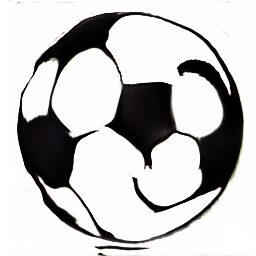
\includegraphics[width=.10\linewidth]{images/autocomplete_generate/scribble/soccer.png}} &
				\frame{
\includegraphics[width=.12\linewidth]{images/face_autocomplete_render/current_scribble_7.jpg}} & 
				\frame{
\includegraphics[width=.12\linewidth]{images/face_autocomplete_render/current_scribble_8.jpg}}&
				\frame{
\includegraphics[width=.12\linewidth]{images/face_autocomplete_render/current_scribble_9.jpg}} &
				\\
				\frame{\includegraphics[width=.12\linewidth]{images/face_autocomplete_render/autocompleted_sketch_6.png}} &
				%\frame{\includegraphics[width=.10\linewidth]{images/autocomplete_generate/scribble/soccer.png}} &
				\frame{\includegraphics[width=.12\linewidth]{images/face_autocomplete_render/autocompleted_sketch_7.png}} & 
				\frame{\includegraphics[width=.12\linewidth]{images/face_autocomplete_render/autocompleted_sketch_8.png}}&
				\frame{\includegraphics[width=.12\linewidth]{images/face_autocomplete_render/autocompleted_sketch_9.png}} &
				
				\\
				\frame{\includegraphics[width=.12\linewidth]{images/face_autocomplete_render/rendered_6.png}} &
				%\frame{\includegraphics[width=.10\linewidth]{images/autocomplete_generate/scribble/soccer.png}} &
				\frame{\includegraphics[width=.12\linewidth]{images/face_autocomplete_render/rendered_7.png}} & 
				\frame{\includegraphics[width=.12\linewidth]{images/face_autocomplete_render/rendered_8.png}}&
				\frame{\includegraphics[width=.12\linewidth]{images/face_autocomplete_render/rendered_9.png}} &
				
				\\
			\end{tabular}
		} 
		
	\end{tabular}
	\vspace{-2mm}
	\caption{\textbf{Example Sketch \& Fill Progression.} The \textbf{first row} represents the progressive addition of new strokes on the canvas, the \textbf{second row} shows the autocompleted sketch, and the \textbf{third row} is the final generated image. 
		As the sparse strokes are changed by the user, the completed shape and generated image evolve as well. Note that changing a stroke locally produces coherent changes in other parts of the image.
		\vspace{-4mm}
	}
	% \es{replace orange and chicken. maybe also moon and cupcake.}}
	\label{fig:autocomplete_generate_sketches}
\end{figure*}

\begin{figure*}[t]
	\centering
	\includegraphics[width=.9\linewidth]{paper_images/cond_comp2.pdf}
	\caption{{\bf Conditioning injection comparison.} We show results across methods on the outline$\rightarrow$image task using the \textbf{SkinnyResNet} architecture. Naive Concatenation \textbf{Concat} often confuses classes, such as oranges and basketballs, while gating mechanisms such as the \textbf{ChannelGate} method succeed. The gating method also improves results for the \textbf{EncoderDecoder} architecture. \label{fig:alg_comp} }
	\vspace{-4mm}
\end{figure*}

\vspace{-4mm}
\section{Experiments}
\label{sec:experiments}
We first compare our 2 step approach for interactive image generation on existing datasets such as the UTZappos Shoes dataset \cite{yu2014fine} and CelebA-HQ \cite{karras2017progressive}. State-of-the-art techniques such as pix2pixHD \cite{Wang_2018_CVPR} are used to generate the final image from the autocompleted sketches. We finally evaluate our approach on a multi-class dataset that we collected to test our proposed gating mechanism.


\begin{table}[t]
	\resizebox{1.\linewidth}{!} {
		\centering
		\begin{tabular}{l c}
			% \hline
			\toprule
			\textbf{Trained task} & \textbf{FID} \\ \midrule
			% PE $\rightarrow$ Image & 73.12 \% \\
			% PO $\rightarrow$ Image & 88.74 \% \\
			% EC $\rightarrow$ FE $\rightarrow$ Image & 45.96 \% \\
			% OC $\rightarrow$ FO $\rightarrow$ Image \textbf{[Ours]} & \textbf{97.38\%}  \\
			\textbf{Faces}\\ \hline
			Partial Simplified Edges $\rightarrow$ Image & 383.02 \\
			Partial Simplified Edges $\rightarrow$ Simplified Edges $\rightarrow$ Image & 374.67 \\
			\hline
			\textbf{Shoes}\\ \hline
			Partial Simplified Edges $\rightarrow$ Image & 170.45 \\
			Partial Simplified Edges $\rightarrow$ Simplified Edges $\rightarrow$ Image & 154.32 \\
			% Partial edges $\rightarrow$ Full edges $\rightarrow$ Image & 45.96 \% \\
			% \cdashline{1-2}
			% Partial outline $\rightarrow$ Full outline $\rightarrow$ Image [Ours] & \textbf{97.38\%}  \\
			\bottomrule %inserts single line
		\end{tabular}
	}
	\vspace{-2mm}
	\caption{\label{table:2step_eval_single_class} \textbf{Single-class generation, 2-stage vs 1-stage}. We evaluate the result quality from different task pipelines.
		% Evaluates the result quality from different trained task pipelines, including Partial Edges (PE), Partial Outlines (PO), Edge Completion (EC), Full Edges (FE), Outline Completion (OC), and Full Outlines (FO). Accuracy is computed by a fixed, pretrained classification network, on the resulting images.
		\vspace{-4mm}
	}
\end{table}
\vspace{-2mm}
\subsection{Single Class Generation}
\paragraph{Datasets} We use the edges2shoes\cite{isola2016image2image}, CelebA-HQ\cite{karras2017progressive} datasets to test our method on single class generation. 
We simplify the edges to attempt to more closely resemble how humans would draw strokes by first using the preprocessing code of \cite{li2019im2pencil} further reducing the strokes with a sketch simplification network \cite{simo2016learning}.
\paragraph{Architecture} We use the architecture described in Section \ref{sec:shape} for shape completion. In this case, each dataset only contains a single class, so we can use an off-the-shelf network, such as pix2pixHD~\cite{wang2017high} for rendering.

\paragraph{Results} As seen in \figref{fig:autocomplete_generate_sketches}, our 2 step technique allows us to complete the simplified edge maps from the partial strokes and also generate realistic images from the autocompleted simplified edges.
Table \ref{table:2step_eval_single_class} also demonstrates, across two datasets (faces and shoes), that using a 2 step procedure produces stronger results than mapping directly from the partial sketch to the completed image.

\begin{table}[t]
	\centering
	\begin{tabular}{l c}
		% \hline
		\toprule
		\textbf{Trained task} & \textbf{Avg Acc} \\ \midrule
		% PE $\rightarrow$ Image & 73.12 \% \\
		% PO $\rightarrow$ Image & 88.74 \% \\
		% EC $\rightarrow$ FE $\rightarrow$ Image & 45.96 \% \\
		% OC $\rightarrow$ FO $\rightarrow$ Image \textbf{[Ours]} & \textbf{97.38\%}  \\
		Partial edges $\rightarrow$ Image & 73.12 \% \\
		Partial outline $\rightarrow$ Image & 88.74 \% \\
		% Partial edges $\rightarrow$ Full edges $\rightarrow$ Image & 45.96 \% \\
		% \cdashline{1-2}
		Partial outline $\rightarrow$ Full outline $\rightarrow$ Image [Ours] & \textbf{97.38\%}  \\
		\bottomrule %inserts single line
	\end{tabular}
	\vspace{-2mm}
	\caption{\label{table:2step_eval} \textbf{Multi-class generation, 2-stage vs 1-stage}. We evaluate the result quality from different task pipelines. Accuracy is computed by a fixed, pretrained classification network, on the resulting images.
		% Evaluates the result quality from different trained task pipelines, including Partial Edges (PE), Partial Outlines (PO), Edge Completion (EC), Full Edges (FE), Outline Completion (OC), and Full Outlines (FO). Accuracy is computed by a fixed, pretrained classification network, on the resulting images.
		\vspace{-1mm}
	}
\end{table}




\begin{figure}[t]%[ht!]
	\centering
	\begin{tabular}{*{6}{c@{\hspace{3px}}}}
		\frame{\includegraphics[width=.15\linewidth]{images/ablation_images/basketball_partial_outline.png}} &
		\frame{\includegraphics[width=.15\linewidth]{images/ablation_images/basketball_full_outline.png}} &
		\frame{\includegraphics[width=.15\linewidth]{images/ablation_images/soccer_partial_outline.png}} & 
		\frame{\includegraphics[width=.15\linewidth]{images/ablation_images/soccer_full_outline.png}}&
		\frame{\includegraphics[width=.15\linewidth]{images/ablation_images/cupcake_partial_outline.png}} &
		\frame{\includegraphics[width=.15\linewidth]{images/ablation_images/cupcake_full_outline.png}}
		\\
		
		\frame{\includegraphics[width=.15\linewidth]{images/ablation_images/basketball_partial_outline_gen.png}} &
		\frame{\includegraphics[width=.15\linewidth]{images/ablation_images/basketball_full_outline_gen.png}} &
		\frame{\includegraphics[width=.15\linewidth]{images/ablation_images/soccer_partial_outline_gen.png}} & 
		\frame{\includegraphics[width=.15\linewidth]{images/ablation_images/soccer_full_outline_gen.png}}&
		\frame{\includegraphics[width=.15\linewidth]{images/ablation_images/cupcake_partial_outline_gen.png}} &
		\frame{\includegraphics[width=.15\linewidth]{images/ablation_images/cupcake_full_outline_gen.png}}
		\\
		
		% \begin{subfigure}[t]{.15\linewidth}\caption{}\label{fig:basketball_partial}\end{subfigure} &
		% \begin{subfigure}[t]{.15\linewidth}\caption{}\label{fig:basketball_full}\end{subfigure} &
		% \begin{subfigure}[t]{.15\linewidth}\caption{}\label{fig:soccer_partial}\end{subfigure} &
		% \begin{subfigure}[t]{.15\linewidth}\caption{}\label{fig:soccer_full}\end{subfigure} &
		% \begin{subfigure}[t]{.15\linewidth}\caption{}\label{fig:cupcake_partial}\end{subfigure} &
		% \begin{subfigure}[t]{.15\linewidth}\caption{}\label{fig:cupcake_full}\end{subfigure}\\
	\end{tabular}
	\caption{\textbf{Directly mapping from partial outline to image} Our proposed system uses a 2-stage approach, using a completed edge map as an intermediate. Here, we show results when directly mapping from the partial outline to the image. When the outline is well-defined, the network can generate realistic images. However, when the outline is sparse, the network struggles with the geometry.}
	\label{fig:ablation_partial_full_outline}
	\vspace{-3mm}
\end{figure}

\begin{figure}[t]%[ht!]
	\centering
	\resizebox{1.0\linewidth}{!}{
		\begin{tabular}{*{5}{c@{\hspace{3px}}}}
			\frame{\includegraphics[width=.2\linewidth]{images/autocomplete_generate/scribble/basketball.png}} &
			%\frame{\includegraphics[width=.10\linewidth]{images/autocomplete_generate/scribble/soccer.png}} &
			\frame{\includegraphics[width=.2\linewidth]{images/autocomplete_generate/scribble/watermelon.png}} & 
			\frame{\includegraphics[width=.2\linewidth]{images/autocomplete_generate/scribble/orange.png}}&
			\frame{\includegraphics[width=.2\linewidth]{images/autocomplete_generate/scribble/cookie.png}} &
			%\frame{\includegraphics[width=.10\linewidth]{images/autocomplete_generate/scribble/moon.png}} &
			%\frame{\includegraphics[width=.10\linewidth]{images/autocomplete_generate/scribble/strawberry.png}} &
			\frame{\includegraphics[width=.2\linewidth]{images/autocomplete_generate/scribble/pineapple.png}}
			%\frame{\includegraphics[width=.10\linewidth]{images/autocomplete_generate/scribble/cupcake.png}} &
			%\frame{\includegraphics[width=.10\linewidth]{images/autocomplete_generate/scribble/chicken.png}}
			\\
			
			\frame{\includegraphics[width=.2\linewidth]{images/autocomplete_generate/autocomplete/basketball.png}} &
			%\frame{\includegraphics[width=.10\linewidth]{images/autocomplete_generate/autocomplete/soccer.png}} &
			\frame{\includegraphics[width=.2\linewidth]{images/autocomplete_generate/autocomplete/watermelon.png}} & 
			\frame{\includegraphics[width=.2\linewidth]{images/autocomplete_generate/autocomplete/orange.png}}&
			\frame{\includegraphics[width=.2\linewidth]{images/autocomplete_generate/autocomplete/cookie.png}} &
			%\frame{\includegraphics[width=.10\linewidth]{images/autocomplete_generate/autocomplete/moon.png}} &
			%\frame{\includegraphics[width=.10\linewidth]{images/autocomplete_generate/autocomplete/strawberry.png}} &
			\frame{\includegraphics[width=.2\linewidth]{images/autocomplete_generate/autocomplete/pineapple.png}}
			%\frame{\includegraphics[width=.10\linewidth]{images/autocomplete_generate/autocomplete/cupcake.png}} &
			%\frame{\includegraphics[width=.10\linewidth]{images/autocomplete_generate/autocomplete/chicken.png}}
			\\
			
			
			\frame{\includegraphics[width=.2\linewidth]{images/autocomplete_generate/image/basketball.png}} &
			%\frame{\includegraphics[width=.10\linewidth]{images/autocomplete_generate/image/soccer.png}} &
			\frame{\includegraphics[width=.2\linewidth]{images/autocomplete_generate/image/watermelon.png}} & 
			\frame{\includegraphics[width=.2\linewidth]{images/autocomplete_generate/image/orange.png}}&
			\frame{\includegraphics[width=.2\linewidth]{images/autocomplete_generate/image/cookie.png}} &
			%\frame{\includegraphics[width=.10\linewidth]{images/autocomplete_generate/image/moon.png}} &
			%\frame{\includegraphics[width=.10\linewidth]{images/autocomplete_generate/image/strawberry.png}} &
			\frame{\includegraphics[width=.2\linewidth]{images/autocomplete_generate/image/pineapple.png}}
			%\frame{\includegraphics[width=.10\linewidth]{images/autocomplete_generate/image/cupcake.png}} &
			%\frame{\includegraphics[width=.10\linewidth]{images/autocomplete_generate/image/chicken.png}}
			\\
			% \begin{subfigure}[t]{.15\linewidth}\caption{}\label{fig:basketball_partial}\end{subfigure} &
			% \begin{subfigure}[t]{.15\linewidth}\caption{}\label{fig:basketball_full}\end{subfigure} &
			% \begin{subfigure}[t]{.15\linewidth}\caption{}\label{fig:soccer_partial}\end{subfigure} &
			% \begin{subfigure}[t]{.15\linewidth}\caption{}\label{fig:soccer_full}\end{subfigure} &
			% \begin{subfigure}[t]{.15\linewidth}\caption{}\label{fig:cupcake_partial}\end{subfigure} &
			% \begin{subfigure}[t]{.15\linewidth}\caption{}\label{fig:cupcake_full}\end{subfigure}\\
		\end{tabular}
	}
	% \vspace{-2mm}
	\caption{\textbf{Multiclass Sketch \& Fill results}
		A few input strokes (first row) are enough to automatically complete the class specific outlines (second) and appearance (last).
		\vspace{-3mm}
	}
	% \es{replace orange and chicken. maybe also moon and cupcake.}}
	\label{fig:autocomplete_generate}
\end{figure}

% \begin{figure}[ht!]
%   \centering
%   \begin{minipage}[t]{\linewidth}  

\begin{table}[]
	\centering
	\resizebox{1.\linewidth}{!} {
		\setlength{\tabcolsep}{6pt}
		\begin{tabular}{l c c c c}
			\toprule
			\multirow{3}{*}{\textbf{Method}} & \multicolumn{2}{c}{ {\bf SkinnyResNet}} & \multicolumn{2}{c}{ {\bf EncDec}} \\ \cmidrule(l){2-3} \cmidrule(l){4-5}
			% 	& \textbf{Accuracy} & \textbf{Realism} & \textbf{Accuracy} & \textbf{Realism} \\
			& Class. & AMT Fool. & Class. & AMT Fool. \\
			& Acc [\%] & Rate [\%] & Acc [\%] & Rate [\%] \\ \midrule
			% 	\cmidrule(l){1-1} \cmidrule(l){2-3} \cmidrule(l){4-5}
			Ground truth & 100.0 & 50.0 & 100.0 & 50.0 \\ \midrule
			1 gen/class & \textbf{\textit{97.0}} & 17.7$\pm$1.46 & -- & -- \\ \midrule
			Concat (In)	& 62.6 & 15.0$\pm$1.4 & 39.2 & 7.5$\pm$1.06 \\ 
			Concat (All) & 64.5 & 15.3$\pm$1.41 & 51.4 & 5.4$\pm$0.88 \\ \midrule
			Cat(In)+Aux-Class & 65.6 & 14.5$\pm$1.5 & -- & -- \\ 
			Cat(All)+Aux-Class & 67.0 & 19.7$\pm$1.42 & -- & --\\ \midrule
			BlockGate(+bias) & 89.6 & 19.6$\pm$1.34 & -- & --\\ 
			BlockGate & {\bf 99.6} & 17.3$\pm$1.61 & -- & --\\ 
			AdaIn & 94.5 & 14.9$\pm$1.47 & -- & --\\ 
			ChanGate(+bias) & 94.1 & 14.8$\pm$1.43 & -- & --\\ 
			ChanGate & \textbf{\textit{97.0}} & {\bf 23.4$\pm$1.99} & 92.7 & 14.1$\pm$1.48 \\ 
			\hline
			\vspace{-5mm}
			\caption{\small {\bf Accuracy vs Realism on Multiclass Outline$\rightarrow$Image task.} We measure generation accuracy with a pretrained network. We measure realism using the real vs. fake judges from AMT. Higher is better for both. Our SkinnyResNet architecture outperforms the Encoder-Decoder network, inspired by MUNIT~\cite{huang2018multimodal}. We perform a thorough ablation on our architecture and find that channel-wise gating achieves high accuracy and higher realism.
				\vspace{-5mm}
			}\label{fig:acc_vs_real}
		\end{tabular} 
	}
\end{table}


\subsection{Multi-Class Generation} 
\paragraph{Datasets} To explore the efficacy of our full pipeline, we introduce a new outline dataset consisting of 200 images (150 train, 50 test) for each of 10 classes -- basketball, chicken, cookie, cupcake, moon, orange, soccer, strawberry,  watermelon and pineapple. All the images have a white background and were collected using search keywords on popular search engines.
% \es{where are images coming from?}
In each image, we obtain rough outlines for the image. We find the largest blob in the image after thresholding it into a black and white image. We fill the interior holes of the largest blob and obtain a smooth outline using the Savitzky–Golay filter~\cite{savitzky1964smoothing}.

\paragraph{Architecture} For the shape completion, we use the architecture in Section \ref{sec:shape}. For class-conditioned image generation, test the gated architectures in Section \ref{sec:appearance}.
\vspace{-4mm}
\paragraph{Results}
In order to test the fidelity of the automatically completed shapes, we evaluate the accuracy of a trained classifier on being able to correctly label a particular generation.
We first test in Table \ref{table:2step_eval} that our 2 stage technique is better than 1 step generation.
We evaluate the results on the multi-class outline to image generations on two axes: adherence to conditioning and realism. We first test the conditioning adherence -- whether the network generates an image of the correct class.
Off-the-shelf networks have been previously used to evaluate colorizations~\cite{zhang2016colorful}, street scenes~\cite{isola2016image2image, wang2017high}, and ImageNet generations~\cite{salimans2016improved}. 
We take a similar approach and fine-tune a pretrained InceptionV3 network~\cite{szegedy2016rethinking} for our 10 classes. 
The generations are then tested with this network for classification accuracy. Results are presented in Table~\ref{fig:acc_vs_real}.

To judge the generation quality, we also perform a ``Visual Turing test" using Amazon Mechanical Turk (AMT). Turkers are shown a real image, followed by a generated image, or vice versa, and asked to identify the fake. An algorithm which generates a realistic image will ``fool" Turkers into choosing the incorrect image. We use the implementation from~\cite{zhang2016colorful}.
Results are presented in Table~\ref{fig:acc_vs_real}, and qualitative examples are shown in Fig.~\ref{fig:alg_comp}.



\paragraph{Gating Architectures}
We compare our proposed model to the residual \textbf{Encoder-Decoder} model~\cite{huang2018multimodal}.
%In addition, we evaluate and analyze different gating variants and report the most effective one in the context of the outline-to-image generation task.
In addition, we compare our proposed gating strategy and {\bf SkinnyResNet} architecture to the following methods for  conditional image generation:

\begin{itemize}[noitemsep,leftmargin=12pt]
	\item{\bf Per-class}: a single generator for each category; this is the only test setting with \textit{multiple} networks, all others train a single network
	\item{\bf Concat (In)}: naive concatenation, input layer only
	\item{\bf Concat (All)}: naive concatenation, all layers
	\item{\bf Concat (In)+Aux-Class}: we add an auxiliary classifier, both for input-only and all layers settings
	\item{\bf BlockGate(+Bias), BlockGate}: block-wise soft-gating, with and without a bias parameter
	\item{\bf AdaIn}: Adaptive instance normalization
	\item{\bf ChannelGate(+Bias), ChannelGate}: channel-wise soft-gating, with and without a bias parameter
\end{itemize}
% AdaIn describes the case where an Instance Normalization~\cite{ulyanovinstance} (IN) operation is applied before scaling and shifting the feature distribution.
% We constrain each element of {\boldmath $\alpha$} and {\boldmath $\beta$} in $[-1, 1]$ %(constraining between [0, 1] did not provide the best empirical results).
\vspace{-2mm}
% \begin{equation}
% X + \mbox{\boldmath $\alpha$} \odot \text{IN} (\mathcal{H}(X)) + \mbox{\boldmath $\beta$}
% \end{equation}


\vspace{2mm} \noindent \textbf{Does naive concatenation effectively inject conditioning?} In Fig.~\ref{fig:alg_comp}, we show a selected example from each of the 10 classes. The per-class baseline trivially adheres to the conditioning, as each class gets to have its own network. However, when a single network is trained to generate all classes, naive concatenation is unable to successfully inject class information, for either network and for either type of concatenation. For the \textbf{EncoderDecoder} network, basketballs, oranges, cupcakes, pineapples, and fried chicken are all confused with each other. For the \textbf{SkinnyResNet} network, oranges are generated instead of basketballs, and pineapples and fried chicken drumsticks are confused. As seen in Table~\ref{fig:acc_vs_real}, classification accuracy is slightly higher when concatenating all layers ($64.5\%$) versus only the input layer ($62.6\%$), but is low for both.


\vspace{2mm} \noindent \textbf{Does gating effectively inject conditioning?} Using the proposed soft-gating, on the other hand, leads to successful generations. We test variants of soft-gating on the \textbf{SkinnyResNet}, and accuracy is dramatically improved, between $89.6\%$ to $99.6\%$, comparable to using a single generator per class ($97.0\%$).
% \pd{Two variants of gating provide accuracy better than per-class generator.}
Among the gating mechanisms, we find that channel-wise multiplication
% (on both generator and discriminator)
generates the most realistic images, achieving an AMT fooling rate of $23.4\%$. Interestingly, the fooling rate is higher than the per-class generator of $17.7\%$. Qualitatively, we notice that per-class generators sometimes exhibits artifacts in the background, as seen in the generation of ``moon". We hypothesize with the correct conditioning mechanism, the single generator across multiple classes has the benefit of seeing more training data and finding common elements across classes, such as clean, white backgrounds.



\vspace{2mm} \noindent \textbf{Is gating effective across architectures?} 
As seen in Table~\ref{fig:acc_vs_real}, using channelwise gating instead of naive concatenation improves performance both accuracy and realism \textit{across} architectures. For example, for the \textbf{EncoderDecoder} architecture, gating enables successful generation of the pineapple.
Both quantitatively and qualitatively, results are better for our proposed \textbf{SkinnyResNet} architecture.

% Yes, works for both skinny resnet \& enc-dec.

\vspace{2mm} \noindent \textbf{Do the generations generalize to unusual outlines?} The training images consist of the outlines corresponding to the geometry of each class. However, an interesting test scenario is whether the technique generalizes to unseen shape and class combinations. In \figref{fig:teaser}, we show that an input circle not only produces circular objects, such as a basketball, watermelon, and cookie, but also noncircular objects such as strawberry, pineapple, and cupcake. Note that both the pineapple crown and bottom are generated, even without any structural indication of these parts in the outline.



\section{Discussion}


We present a two-stage approach for interactive object generation, centered around the idea of a shape completion intermediary. This step both makes training more stable and also allows us to give coarse geometric feedback to the user, which they can choose to integrate as they desire. 
\chapter{STEER: Simple Temporal Regularization For Neural ODEs}
%\subimport{papers/steer/}{neurips_2020}

\begin{abstract}
	Training Neural Ordinary Differential Equations (ODEs) is often computationally expensive. Indeed, computing the forward pass of such models involves solving an ODE which can become arbitrarily complex during training. Recent works have shown that regularizing the dynamics of the ODE can partially alleviate this. In this paper we propose a new regularization technique: randomly sampling the end time of the ODE during training. The proposed regularization is simple to implement, has negligible overhead and is effective across a wide variety of tasks. Further, the technique is orthogonal to several other methods proposed to regularize the dynamics of ODEs and as such can be used in conjunction with them. We show through experiments on normalizing flows, time series models and image recognition that the proposed regularization can significantly decrease training time and even improve performance over baseline models.
\end{abstract}

\section{Introduction}
\begin{figure}
	\centering
	\begin{tabular}{*{4}{c@{\hspace{3px}}}}
		\includegraphics[width=0.48\linewidth]{images/main_figure/neural_ode.png}  & 
		\includegraphics[width=0.48\linewidth]{images/main_figure/neural_ode_steer.png}
		\\
	\end{tabular}
	\caption{Flow fields of a standard Neural ODE (left) vs one equipped with STEER (right). These models transform a simple initial distribution $p(z_{t_0})$ to the target distribution $p(z_{t})$. STEER learns simpler flows, which enable faster training.}
	\label{fig:main_steer}
\end{figure}

Neural Ordinary Differential Equations (ODE) are an elegant approach for building continuous depth neural networks \cite{chen2018neural}. They offer various advantages over traditional neural networks, for example a constant memory cost as a function of depth and invertibility by construction. %
As they are inspired by dynamical systems, they can also take advantage of the vast amount of mathematical techniques developed in this field.
Incorporating continuous depth also enables efficient density estimation \cite{grathwohl2018ffjord} and modeling of irregularly sampled time series \cite{rubanova2019latent}.

The aforementioned advantages come at the expense of a significantly increased computational cost compared with traditional models like Residual Networks \cite{he2016deep}.
The training dynamics of Neural ODEs become more complicated as training progresses and the number of steps taken by the adaptive ODE solver (typically referred to as the number of function evaluations) can become prohibitively large \cite{dupont2019augmented}. In fact, several works have argued that this is one of the most pressing limitations of Neural ODEs \cite{chen2018neural, dupont2019augmented, finlay2020train}. It is therefore important to design methods that can help reduce the computational cost of this tool.

A natural approach for tackling this issue is to explore regularization techniques that simplify the underlying dynamics for these models. Indeed, simpler dynamics have shown benefits in terms of faster convergence and a lower number of function evaluations both during training and testing \cite{dupont2019augmented}.
\cite{finlay2020train} recently proposed an interesting technique for explicitly regularizing the dynamics based on ideas from optimal transport showing significant improvements in the effective convergence time.
In this work, we propose a regularization technique in order to further accelerate training. Our regularization is orthogonal to previous approaches and can therefore be used in conjunction with them. Our technique is extremely simple: during training we randomly sample the upper limit of the ODE integration.



Specifically, the solver in Neural ODEs takes as input the integration limits $(t_0,t_1)$.
We propose to introduce regularization by randomly perturbing the end time parameter $t_1$ to be $t_1\pm \delta$ where $\delta$ is a random variable.
% We show that our approach is theoretically valid by proving the existence of the solution for our perturbed ODE.
Empirically, we demonstrate that, in a wide variety of tasks, the proposed regularization achieves comparable performance to unregularized models at a significantly lower computational cost. We test our regularization technique on continuous normalizing flows \cite{grathwohl2018ffjord}, irregularly sampled time series \cite{rubanova2019latent} and image recognition tasks and show that it improves performance across all these tasks. It also performs better in certain instances of Stiff ODEs. Stiff ODEs are a widely studied topic in the field of engineering\cite{curtiss1952integration}. During training the dynamics learnt by the implicit model parametrized by the neural network can turn into an instance of a Stiff ODE. Techniques which could tackle the instances of Stiff ODE would prove to be instrumental as these implicit deep learning models mature. 



\section{Related Work}
Connections between deep neural networks and dynamical systems were made as early as \cite{lagaris1998artificial}. The adjoint sensitivity technique was explored in \cite{pearlmutter1995gradient}. Some early libraries such as dolfin \cite{farrell2013automated,rackauckas2017differentialequations}, implemented the adjoint method for neural network frameworks. Previous works have shown the connection between residual networks and dynamical systems \cite{ruthotto2019deep,haber2017stable,lu2017beyond, weinan2017proposal,wang2019resnets, avelin2019neural}. By randomly dropping some blocks of a residual network, it was demonstrated that deep neural networks could be trained \cite{huang2016deep} or tested \cite{veit2016residual,ghosh2019interactive}
with stochastic depth, and that such a training procedure produces ensembles of shallower networks. 

Neural ODEs \cite{chen2018neural} introduced a framework for training ODE models with backpropagation. Recent works \cite{massaroli2020dissecting, zhang2019approximation, cuchiero2019deep, jabir2019mean, massaroli2020stable, davis2020time, hanshu2019robustness,norcliffe2020second} have tried to analyze this framework theoretically and empirically. Neural ODEs were extended to work with flow based generative models \cite{grathwohl2018ffjord}. In contrast to standard flow based models such as \cite{kingma2018glow, dinh2016density, papamakarios2017masked, papamakarios2019normalizing}, continuous normalizing flows do not put any restrictions on the model architecture. 
Furthermore, Neural ODEs have been applied in the context of irregularly sampled time series models \cite{rubanova2019latent}, reinforcement learning \cite{du2020model} and for set modeling\cite{li2020exchangeable}. Neural ODEs have also been explored for harder tasks such as video generation \cite{yildiz2019ode2vae,kanaasimple} and for modeling the evolving dynamics of graph neural networks \cite{xhonneux2019continuous}. 
Recent work has also extended Neural ODEs to stochastic differential equations \cite{li2020scalable, liu2019neural, hodgkinson2020stochastic, oganesyan2020stochasticity, wu2020stochastic, jia2019neural}.

The methods most relevant to our work are \cite{kelly2020learning, finlay2020train} and \cite{dupont2019augmented}. A regularization based on principles of optimal transport which simplifies the dynamics of continuous normalizing flow models, was introduced in \cite{finlay2020train} to make training faster. Equations which are easier to learn were analyzed in \cite{kelly2020learning} whereby they used a differential surrogate for the time cost of standard numerical solvers, using higher-order derivatives of solution trajectories.  Augmented Neural ODEs \cite{dupont2019augmented} introduced a simple modification to Neural ODEs by adding auxillary dimensions to the ODE function and showing how this simplified the dynamics. Our work is complementary to these methods, and we empirically demonstrate that our method can be used to further improve the performance of these techniques.

There is a huge treasure of work which deals with instability in training ODEs\cite{dahlquist198533,dahlquist1976error}. Curtiss et al. \cite{curtiss1952integration} were one of the first works that dealt with solving stiff equations. It was observed in Curtiss and Hirschfelder \cite{curtiss1952integration} that explicit methods failed for the numerical solution of ordinary differential equations that model certain chemical reactions. It is very difficult to integrate "stiff" equations by ordinary numerical methods. Small errors are rapidly magnified if the equations are integrated. The other case might be that the errors oscillate rapidly. Implicit methods such as the second order Adams-Moulton (AM2) \cite{wanner1996solving} are elegant techniques which deal with some of the problems of stiff ODEs. In the context of Neural ODEs\cite{chen2018neural} implicit computations reduces the efficiency of the solvers. This effect is especially apparent in complex modeling tasks such as generative modeling using continuous normalizing flows\cite{grathwohl2018ffjord} and irregularly sampled timeseries models\cite{rubanova2019latent}. Hence an analysis of simple scenarios of stiff equations which cause problems for standard Neural ODEs are discussed in the following sections.  
% Stiff ODEs have been extensively researched in the field of differential equations \cite{brugnano2011fifty}. Inspite of years of research a concrete definition of Stiff ODEs hasn't been agreed upon \cite{soderlind2015stiffness}. We highlight how some of the problems of Stiff ODEs could impact the training dynamics of Neural ODEs in specific scenarios. Certain discussions of Stiff ODEs define that the stiffness concerns the underlying mathematical form of the equation, integration time and a set of initial data.


\section{Methodology}

\subsection{Neural ODEs}
Neural ODEs can be interpreted as a continuous equivalent of Residual networks \cite{he2016deep}. The transformation of a residual layer is $\mathbf{z}_{t+1}= \mathbf{z}_t + f_t(\mathbf{z}_t)$, where the representation at layer $t$ is $\mathbf{z}_t$ and $f_t( \mathbf{z}_t)$ is a function parametrized by a neural network. The output dimension of the function $f_t(\mathbf{z}_t)$ should be the same as the input dimension to allow it to be added to the previous layer's features $\mathbf{z}_t$. This transformation can be rewritten as

\begin{equation}
	\frac{\mathbf{z}_{t+\delta_t}-\mathbf{z}_t}{ \delta_t } = f_t(\mathbf{z}_t) , \; \; \; \delta_t = 1,
	\label{eq:resnet}
\end{equation}

which can be interpreted as finite difference approximation of the derivative. In contrast to traditional deep neural networks where $\delta_t=1$ is fixed, Neural ODEs \cite{chen2018neural} introduced a continuous version by analysing \eqnref{eq:resnet} in the limit $\delta_t \rightarrow 0$. The resulting equation becomes 

\begin{equation}
	\frac{d\mathbf{z}(t)}{dt} = f(\mathbf{z}(t),t).
	\label{eq:neural_ode_def}
\end{equation}

To transform an input $\mathbf{x}$ to an output $\mathbf{y}$, Residual networks use a sequence of $k$ functions to transform the representation. In an analogous manner, Neural ODEs evolve the  representation from the initial time $t=t_0, \; \mathbf{z}(t_0)= \mathbf{x}$, to the final time $t=t_1, \; \mathbf{z}(t_1)= \mathbf{y}$. The representation $\mathbf{z}(t)$ at any given time $t$ can then be obtained by solving \eqnref{eq:neural_ode_def} using an off-the-shelf ODE solver with the function $f(\mathbf{z}(t),t)$ parameterized by the neural network. To update the parameters of the function $f(\mathbf{z}(t),t)$ such that $\mathbf{z}(t_1) \approx \mathbf{y}$ we backpropagate through the operations of the ODE solver to obtain the appropriate gradients.



\subsection{Temporal Regularization}
The formulation of a standard Neural ODE is given by

\begin{equation}
	\mathbf{z}(t_1)= \mathbf{z}(t_0) + \int_{t_0}^{t_1} f(\mathbf{z}(t) , t , \mathbf{\theta}) dt = \text{ODESolve}  (\mathbf{z}(t_0) , f , t_0, t_1 , \mathbf{\theta}  ),
	\label{eq:ode_formulation}
\end{equation}

where $\mathbf{z}(t)$ is the latent representation at any time $t$. $\mathbf{\theta}$ are the parameters of the function $f$ and $(t_0, t_1)$ are the limits of the integration. The initial condition of the ODE is set as $\mathbf{z}(t_0)=\mathbf{x}$. 


Neural ODEs often take an excessively large time to train, especially in the case of continuous normalizing flows \cite{grathwohl2018ffjord} . The dynamics become more complicated as training progresses thus leading to an increase in the number of function evaluations. In the context of Neural ODEs, the dynamics of the ODE and training time are intricately related. In practice, simpler dynamics \cite{dupont2019augmented, finlay2020train} often lead to faster training with fewer function evaluations. Regularization is commonly used in machine learning to ease the training of a model and improve its generalization. Some common instances include Batchnorm \cite{ioffe2015batch} and early stopping \cite{yao2007early}. 




Neural ODEs continuously evolve the representation $\mathbf{z}(t)$ with time $t$. Thus in the context of neural ODEs, an alternative type of regularization is possible, namely temporal regularization. In this work, we propose a simple regularization technique that exploits this temporal property. We propose to perturb the final time $t_1$ for the integration of the Neural ODE in \eqnref{eq:ode_formulation} during training. At each training iteration, the final time $t_1$ for the integration is stochastically sampled. More formally, if we assume $t_0<t_1$, then our regularization can be formulated as 
\begin{equation}
	\begin{split}
		\label{skip_formulation}
		\mathbf{z}(t_1) &= \mathbf{z}(t_0) + \int_{t_0}^{T} f(\mathbf{z}(t) , t , \theta) dt = \text{ODESolve}(\mathbf{z}(t_0) , f , t_0, T , \theta  ), \\
		T &\sim \text{Uniform} ( t_{1}-b, t_{1}+ b ),  \\
		b &< t_1-t_0 :  \text{parameter controlling interval of uniform distribution}. \\
	\end{split}
\end{equation}


\begin{figure}
	\centering  
	\frame{\includegraphics[trim=2cm 16cm 3cm 7cm, clip=true,width=0.9\linewidth]{images/models/behavior.pdf}} 
	\caption{Effective behavior of Neural ODEs with STEER regularization. The solution is reached at a time $t_1-b$ instead of time $t_{1}$.}
	\label{fig:behavior}
\end{figure}

We call the technique STEER, which stands for Simple Temporal Regularization. 
Since Neural ODEs model a continuous series of transformations, applying STEER is essentially equivalent to performing a variable number of transformations on the input $\mathbf{x}$ in each training iteration, thereby introducing a new form of stochasticity in the training process.

We observe that the proposed regularization effectively ensures convergence to the solution at time $t_1-b$. The effective behavior of $\mathbf{z}(t)$ can be see in \figref{fig:behavior} 

\subsection{Stiff ODEs} 
\label{subsection:stiff_ode}

Stiff ODEs have been extensively researched in the field of differential equations \cite{brugnano2011fifty}. Inspite of years of research a concrete definition of Stiff ODEs has not been agreed upon \cite{soderlind2015stiffness}. We highlight how some of the problems of Stiff ODEs could impact the training dynamics of Neural ODEs in specific scenarios. Certain discussions of Stiff ODEs define that the stiffness concerns the underlying mathematical form of the equation, integration time and a set of initial data.

In terms of the mathematical equation, stiffness is a problem that can arise when numerically solving ODEs. In such systems there is typically a fast and a slow transient component which causes adaptive ODE solvers to take exceedingly small steps. This increases the number of function evaluations and the time taken to integrate the function. %
Furthermore, in Neural ODEs, the function $\frac{d \mathbf{z} }{ dt }$ is parameterized by a neural network which is updated during training, and could become stiff. This would be hard for a traditional ODE solver to integrate efficiently, thereby making this a limitation.


Stiffness ratio is one of the techniques used to characterize some forms of stiff equations. The stiffness ratio is used to characterize the stiffness for the general case of linear constant coefficient systems. These systems can be represented as 
\begin{equation}
	\frac{d \mathbf{z} }{ dt } = \mathbf{Az} + f(t),
	\label{eq:stiff}
\end{equation}
where $\mathbf {z} ,f(t) \in \mathbb{R} ^{n}$ and $\mathbf {A}$ is a $n\times n$ matrix with eigenvalues  $\lambda_{i}\in \mathbb{C} ,i=1,2,\ldots ,n$ (assumed distinct) and corresponding eigenvectors  $\mathbf {c_{i}} \in \mathbb{C} ^{n},i=1,2,\ldots ,n$. The eigenvalues and eigenvectors can be complex. 
The general solution of \eqnref{eq:stiff} takes the form
\begin{equation}
	\mathbf {z}(t)=\sum_{i=1}^{n}\kappa_{i}\exp(\lambda _{i}t) \mathbf{c}_{i}+ \mathbf{g}(t) .
\end{equation}

If $\lambda_{i}$ is complex, the term $\exp(\lambda _{i}t)$ varies sinusoidally. The stiffness ratio is defined as $\frac{\text{max}_{i=1 \dots n} |Re(\lambda_{i})|}{ \text{min}_{i=1 \dots n}|Re(\lambda_{i})|}$, where $Re(\lambda_i)$ denotes the real component of $\lambda_i \in \mathbb {C}$. Ordinarily, temporal regularization might fail in the face of stiffness. However, in our empirical experiments we observed that at least in the case of toy problems, STEER actually performed better. This analysis is provided in the next section. %In the next section, we show how STEER can help tackle stiffness for a range of stiffness ratios on a toy problem where Neural ODEs struggle.



\section{Experiments}
In this section, we demonstrate the effectiveness of the proposed method on several classes of problems.  First, we conduct experiments on continuous normalizing flow based generative models, and compare against FFJORD \cite{grathwohl2018ffjord} and RNODE \cite{finlay2020train}. 
Then, we conduct experiments on irregularly sampled time-series models, and compare against the models and baselines proposed in Latent ODEs \cite{rubanova2019latent}. 
We also conduct experiments on feedforward models for image recognition, and compare against Neural ODEs and Augmented Neural ODEs \cite{dupont2019augmented}. We finally evaluate STEER and standard Neural ODEs on a toy stiff ODE experiment.

\begin{figure}[]
	\centering
	\begin{tabular}{*{4}{c@{\hspace{3px}}}}
		\includegraphics[width=0.32\linewidth]{images/paths_b_comparison/particle_trajectory_0.png} & 
		\includegraphics[width=0.32\linewidth]{images/paths_b_comparison/particle_trajectory_25.png} &
		\includegraphics[width=0.32\linewidth]{images/paths_b_comparison/particle_trajectory_375.png} &
		\\
		$b=0$ & $b=0.25$ & $b=0.375$ \\
	\end{tabular}
	\caption{Plots showing the path taken by FFJORD with STEER regularization. STEER regularization ($b=0.25$ and $b=0.375$) performs the same transformation in shorter paths.}
	\label{fig:path_b_comparison}
\end{figure}



\subsection{Generative Models}
Continuous normalizing flow based generative models \cite{grathwohl2018ffjord, chen2018neural} provide an alternate perspective to generative modeling. 
Let $ p( \mathbf{x} )$ be the likelihood of a datapoint $\mathbf{x}$ and $p( \mathbf{z} )$ be the likelihood of the latent $\mathbf{z}$. 
FFJORD \cite{grathwohl2018ffjord} showed that under certain conditions the change in log probability also follows a differential equation $\frac{d \log(p( \mathbf{z}(t)))}{d t} = -\text{tr} \left( \frac{df}{d \mathbf{z} (t)} \right)$. Thus the total change in log probability can be obtained by integrating the equation which leads to %
\begin{equation}
	\log p( \mathbf{z} (t_1)) = \log p( \mathbf{z} (t_0)) - \int_{t_0}^{t_1} \text{tr} \left( \frac{df}{d \mathbf{z} (t)} \right) dt.  
\end{equation}
This allows to compute the point $\mathbf{z_0}$ which generates a given datapoint $\mathbf{x}$, and $\log p( \mathbf{x} )$ under the model by solving the initial value problem:
\begin{align}\label{eq:reverseivp} 
	\underbrace{\begin{bmatrix}
			\mathbf{z_0} \\ \log p(\mathbf{x}) - \log p_{\mathbf{z_0}}(\mathbf{z_0})
	\end{bmatrix}}_{\textnormal{solutions}} = \underbrace{\int_{T}^{t_0}
		\begin{bmatrix}
			f( \mathbf{z} (t), t; \theta) \\ - \text{tr} \left( \frac{df}{d \mathbf{z}(t)} \right) 
		\end{bmatrix}dt}_{\textnormal{dynamics}},\qquad
	\underbrace{\begin{bmatrix}
			\mathbf{z}(T) \\ \log p(\mathbf{x}) - \log p(\mathbf{z}(T))
		\end{bmatrix} = 
		\begin{bmatrix}
			\mathbf{x} \\ \mathbf{0}
	\end{bmatrix}  }_{\textnormal{initial values}} .
\end{align}
The combined dynamics of $\mathbf{z}(t)$ and the log-density of the sample is integrated backwards in time from $T$ to $t_0$. The log likelihood $\log p(\mathbf{x})$ can be computed by adding $\log p_{\mathbf{z_0}}(\mathbf{z_0})$ to the solution of \eqnref{eq:reverseivp}. A major drawback of continuous normalizing flow based models is extremely slow convergence.
STEER regularization enables faster convergence by sampling $T \sim \text{Uniform}(t_1-b,t_1+b)$ at each iteration.

We focus on the task of density estimation of image datasets using the same architectures and experimental setup as FFJORD  \cite{grathwohl2018ffjord}. More details are provided in the supplementary material.
The performance of the model is evaluated on multiple datasets, namely MNIST \cite{lecun1990handwritten}, CIFAR-10 \cite{krizhevsky2009learning} and ImageNet-32 \cite{Deng09ImageNet}, and the results are shown in \tabref{tab:cnf_results}.  The performance is also analyzed in the simple scenario of a 1D Mixture of Gaussians as shown in \figref{fig:path_b_comparison}. 

\begin{table}
	\centering
	\resizebox{\columnwidth}{!}{%
		\begin{tabular}{l c c c c c c}
			\toprule
			& \multicolumn{2}{c}{MNIST} & \multicolumn{2}{c}{CIFAR-10} & \multicolumn{2}{c}{IMAGENET-32}\\
			& BITS/DIM & TIME & BITS/DIM & TIME & BITS/DIM & TIME \\
			\midrule
			FFJORD, VANILLA. &  $0.974$ & $68.47$ & $3.40$ & $> 5$ days & $3.96$ & $>5$ days\\
			FFJORD RNODE. \cite{finlay2020train} & $0.973$ & $24.37$ & $3.398$ & $31.84$ & $2.36$ & $30.1$ \\
			\hdashline
			FFJORD, VANILLA. + STEER ($b=0.5$) &  $0.974$ & $51.21$ & $3.40$ & $86.34$ & $3.84$ & $>5$ days \\
			FFJORD, VANILLA. + STEER ($b=0.25$) &  $0.976$ & $58.21$ & $3.41$ & $103.4$ & $3.87$ & $>5$ days \\
			FFJORD RNODE + STEER ($b=0.5$) & $\mathbf{0.971}$ & $\mathbf{16.32}$ & $\mathbf{3.397}$ & $\mathbf{22.24}$ & $\mathbf{2.35}$ & $\mathbf{24.9}$ \\
			FFJORD RNODE + STEER ($b=0.25$) & $0.972$ & $19.71$ & $3.401$ & $25.24$ & $2.37$ & $27.84$ \\
			\bottomrule %
		\end{tabular}
	}
	\caption{Test accuracy and training time comparison on various image datasets. Unless mentioned as days, the time reported is in hours.}  %
	\label{tab:cnf_results}
\end{table}

It can be seen in \tabref{tab:cnf_results} that models with STEER regularization converge much faster. In some cases, such as on CIFAR-10, our model is $30\%$ faster than the state of the art.

\figref{fig:path_b_comparison} shows the evolution of the probability distribution from the latent distribution $p(\mathbf{z})$ to the data distribution $p(\mathbf{x})$ at different test times. It can be seen that the trajectories reach the final states at an earlier test time with STEER regularization.


\begin{table}
	\small{
		\parbox{.48\textwidth}{
			\centering
			\begin{tabular}{l c}
				\toprule
				\textbf{Model} & \textbf{Accuracy} \\ \midrule
				Latent ODE (ODE enc) & $0.846 \pm 0.013$ \\
				Latent ODE (RNN enc.) &  $0.835 \pm 0.010$ \\
				ODE-RNN &  $0.829 \pm 0.016$ \\
				\midrule
				Latent ODE (ODE enc, STEER) & $\mathbf{0.880 \pm 0.011}$ \\ 
				Latent ODE (RNN enc, STEER) & $0.865 \pm 0.021$ \\ 
				ODE-RNN (STEER) & $0.872 \pm 0.012$ \\ 
				\bottomrule %
			\end{tabular}
			\caption{Per-time-point classification accuracies on the Human Activity dataset.}
			\label{tab:latent_ode_human_activity}
		}
		\hfill
		\parbox{.48\textwidth}{
			\centering
			\begin{tabular}{l c}
				\toprule
				\textbf{Model} & \textbf{AUC} \\ \midrule
				Latent ODE (ODE enc) & $0.829 \pm 0.004$ \\
				Latent ODE (RNN enc.) &  $0.781 \pm 0.018$ \\
				ODE-RNN & $\mathbf{0.833 \pm 0.009}$ \\
				\midrule
				Latent ODE (ODE enc, STEER) & $0.810 \pm 0.018$ \\ 
				Latent ODE (RNN enc, STEER) & $0.772 \pm 0.014$ \\ 
				ODE-RNN (STEER) & $0.811 \pm 0.007$ \\ 
				\bottomrule %
			\end{tabular}
			\caption{Per-sequence classification AUC on Physionet.}
			\label{tab:latent_ode_physionet}
			
		}
	}
\end{table}

\begin{table}
	\centering
	\resizebox{\columnwidth}{!}{
		\begin{tabular}{l | c c c c | c c c c}
			\toprule
			& \multicolumn{4}{c}{Interpolation (\% Observed Pts.)} & \multicolumn{4}{c}{Extrapolation (\% Observed Pts.)}\\
			Model & 10 \% & 20 \% & 30 \% & 50 \% & 10 \% & 20 \% & 30 \% & 50 \% \\
			\midrule
			
			Latent ODE (ODE enc) & $0.360$ &  $0.295$ &  $0.300$ & $0.285$ & $1.441$ & $1.400$ & $1.175$ & $1.258$ \\
			Latent ODE (RNN enc.) & $2.477$ & $0.578$ & $2.768$ & $0.447$ & $1.663$ & $1.653$ & $1.485$ & $1.377$ \\
			ODE-RNN & $1.647$ & $1.209$ & $0.986$ & $0.665$ & $13.508$ & $31.950$ & $15.465$ & $26.463$ \\
			\midrule
			Latent ODE (ODE enc, STEER) & $\mathbf{0.230}$ &  $\mathbf{0.235}$ &  $\mathbf{0.246}$ & $\mathbf{0.210}$ & $\mathbf{1.01}$ & $\mathbf{0.98}$ & $\mathbf{1.01}$ & $\mathbf{1.04}$ \\
			Latent ODE (RNN enc., STEER) & $2.31$ & $0.561$ & $2.534$ & $0.386$ & $1.541$ & $1.498$ & $1.236$ & $1.119$ \\
			ODE-RNN (STEER) & $1.528$ & $1.09$ & $0.796$ & $0.603$ & $11.508$ & $29.34$ & $14.23$ & $23.528$ \\
			\bottomrule %
		\end{tabular}
	}
	\caption{Test Mean Squared Error (MSE) ($ \times 10^{-2}$
		) on the MuJoCo dataset.}
	\label{tab:mujoco_results}
\end{table}

\subsection{Times Series Models}



For time series models, the function is evaluated at multiple times $t_0,..t_n$. We employ the regularization between every consecutive pair of points $(t_i,t_{i+1})$. More formally, if the time is split into consecutive intervals $ (t_0,t_1)...(t_{n-1},t_n)$, we start with $t_0$ and the initialization $\mathbf{z}(t_0)$ and sample the end time as $T \sim \text{Uniform}(t_1-b,t_1+b)$. The resulting integration using the ODE solver gives us the latent representation $\mathbf{z}(t_1)$. We repeat the same procedure where the limits of integration are now $(t_1,t_2)$. In this iteration $t_1$ is not altered while $T \sim \text{Uniform}(t_2-b,t_2+b)$ is sampled to obtain $\mathbf{z}(t_2)$  and so on. 
In the case of irregularly sampled time series models, the length of the interval $t_{i+1}-t_i$ can itself vary. The parameter $b$ in this case is adaptive such that $b=|t_{i+1}-t_i|-\epsilon$. The $\epsilon$ parameter is added to avoid numerical instability issues. In the case of time series models the parameter $b$ changes at each forward pass thus adding another source of stochasticity.  %

Latent ODEs \cite{rubanova2019latent} introduced irregularly sampled time series models in which Neural ODEs perform much better. Indeed these datasets break the basic assumptions of a standard RNN, namely that the data are not necessarily collected at regular time intervals. This is the case in several real life scenarios such as patient records or human activity recognition which are observed at irregularly sampled timepoints. 

The Mujoco experiments consist of a physical simulation of the "Hopper" model from the Deepmind control suite. %
The initial condition uniquely determines the trajectory. It consists of $10,000$ sequences of $100$ time points each. 
The Human Activity dataset \cite{rubanova2019latent} consists of sensor data fitted to individuals. The sensor data is collected using tags attached to the belt, chest and ankles of human performers. It results in $12$ features in total. The task involves classifying each point as to which activity was being performed. Physionet \cite{silva2012predicting} consists of time series data from initial $48$ hours of ICU admissions. It consists of sparse measurements where only some of the features' measurements are taken at an instant. The measurement frequency is also irregular which makes the dataset quite challenging. To predict mortality, binary classifiers were constructed by passing the hidden state to a $2$ layer binary classifier.

We use the same architecture and experiment settings as used in Latent ODEs \cite{rubanova2019latent}. For the Mujoco experiment $15$ and $30$ latent dimensions were used for the generative and recognition models respectively. The ODE function had $500$ units in each of the $3$ layers. A $15$ dimensional latent state was used for the Human Activity dataset.  For the Physionet experiments the ODE function has $3$ layers with $50$ units each. The classifier consisted of $2$ layers with $300$ units each. 


In the case of irregularly sampled timeseries with Latent ODEs, the number of function evaluations is not a major concern since the training time is quite small, so we compare only in terms of accuracy. It can be seen in \tabref{tab:latent_ode_human_activity} and \tabref{tab:mujoco_results} that STEER regularization consistently improves the performance of ODE based models.  \tabref{tab:mujoco_results} demonstrates that the extrapolation results are much better with STEER regularization, indicating that it may help improve the generalization of the model. However in the case of Physionet \tabref{tab:latent_ode_physionet}, the results do not improve over standard Neural ODEs, although the performance remains very close. 

\begin{table}
	\centering
	\begin{tabular}{l c c c c}
		\toprule
		& NODE & NODE(STEER) & ANODE & ANODE(STEER) \\ \midrule
		MNIST & $97.2\% \pm 0.2$ & $98.3\% \pm 0.3 $& $98.2\% \pm 0.1$ & $\mathbf{98.6\% \pm 0.3} $ \\
		CIFAR-10 & $53.7\% \pm 0.4$ & $54.9\% \pm 0.5$ & $60.6\% \pm 0.4$ & $\mathbf{62.1\% \pm 0.2}$      \\
		SVHN &  $81.0\% \pm 0.6$ & $81.8\% \pm 0.3$  & $83.5\% \pm 0.5$  & $\mathbf{84.1 \pm 0.2}$\\
		\bottomrule %
	\end{tabular}
	\caption{Test accuracies on Feedforward models on various datsets.}
	\label{tab:recognition_accuracies}
\end{table}
\subsection{Feedforward Models}
In feedforward learning for classification and regression, the Neural ODE framework can be used to map the input data $\mathbf{x} = \mathbf{z}(t_0) \in \mathbb{R}^d$ to features $\mathbf{z}(t) \in \mathbb{R}^d$ at any given time $t$. For standard neural ODEs, one integrates in the range $(t_0,t_1)$, and for STEER the integration is performed in the range $(t_0,T)$ where $T \in \text{Uniform}(t_1-b,t_1+b)$. Once the features $\mathbf{z}(T)$ at the final time $T$ are obtained, a linear layer $\mathbb{R}^d \rightarrow \mathbb{R}$ is used to map the features to the correct dimension for downstream tasks such as classification or regression.


We evaluate STEER on a similar set of experiments as performed in \cite{dupont2019augmented} on the MNIST \cite{lecun1990handwritten}, CIFAR-10 \cite{krizhevsky2009learning} and SVHN \cite{Netzer11SVHN} datasets using convolutional architectures for $f(\mathbf{z}(t), t)$. We use the same architectures and experimental settings as used in \cite{dupont2019augmented} for both Neural ODEs (NODE) and Augmented Neural ODEs (ANODE). 
For the MNIST experiments, $92$ filters were used for NODEs while $64$ filters were used for ANODEs to compensate for $5$ augmented dimensions. For the CIFAR-10 and SVHN experiments, $125$ filters were used for NODEs while $64$ filters were used for ANODEs with $10$ augmented dimensions. Such a design was employed to ensure a roughly similar number of parameters for a fair comparison.



\tabref{tab:recognition_accuracies} demonstrates the performance of STEER regularization with $b=0.99$. STEER provides a small boost in accuracy and performs consistently across all datasets. 



\subsection{A Toy Example of Stiff ODE}

In this experiment, we analyze a toy example of stiff ODE from \cite{chapra2010numerical}. The aim of this experiment is to highlight the vulnerability of Neural ODEs to stiffness. The experimental setting for section 4.4 was similar to the one used in the official github repository \footnote{https://github.com/rtqichen/torchdiffeq/blob/master/examples/ode\_demo.py} of Neural ODE. Instead of using a 2-D ODE we used a 1-D ODE to be able to better visualize and analyze the behavior. We used Eq 12 in the paper as mentioned in the numerical methods book by \cite{chapra2010numerical} on page 752. It was surprising that a Neural ODE was able to model a 2 dimensional model with ease while the stiff equation was extremely hard for the Neural ODE to model.

The ODE is given by 
\begin{equation}
	\frac{dy}{dt}= -1000y + 3000 - 2000e^{-t},
	\label{eq:stiff}
\end{equation}



\begin{figure}
	\centering
	\begin{tabular}{*{4}{c@{\hspace{3px}}}}
		\includegraphics[width=0.48\linewidth]{images/results/stiff-experiments/neural_ode_single_clear.png} &
		\includegraphics[width=0.48\linewidth]{images/results/stiff-experiments/neural_ode_steer_single_clear.png}
		\\
	\end{tabular}
	\caption{Standard Neural ODE struggles while STEER regularization helps to fit a stiff ODE with stiffness ratio $r=1000$.}
	\label{fig:toy_steer}
\end{figure}

with the initial condition of $y(0)=0$. 
The solution for the above stiff ODE is  $y = 3 - 0.998e^{-1000t} -2.002 e^{-t}$.
We use a simple architecture with a single hidden layer of dimension $500$ for both the standard Neural ODE and the one with STEER. The effective input dimension is $2$ resulting by concatenating $y$ and $t$, and the output dimension is $1$. 


\begin{figure}
	\centering
	\includegraphics[width=0.55\textwidth]{images/results/stiff-experiments/stiffness_comparisons.png}
	\caption{Model with STEER regularization achieves a much lower MSE on a Stiff ODE as the stiffness ratio increases.} 
	\label{fig:stiffness_comparisons}
\end{figure}

As shown in \figref{fig:toy_steer}, the solution is initially dominated by the fast exponential term $e^{-1000t}$. After a short period $(t<0.005)$, this transient dies down and the solution is dictated by the slow exponential $e^{-t}$. 
The training interval $[0,15]$ is broken down into small intervals of length $(t_1-t_0)=0.125$. We sample 1000 random initial points $t_0$ and use $y(t_0)$ as the initialization and then try to estimate the value of the function $y(t_1)$ at $t_1=t_0+0.125$.
It can be seen in \figref{fig:toy_steer} that standard Neural ODE doesn't show the same asymptotic behavior as the actual solution, whereas STEER regularization enables better asymptotic behavior. The minimum Mean Squared Error(MSE) loss over all the points of the trajectory in the test interval $[0,25]$ for standard Neural ODE is $3.87$, and with STEER regularization with $b=0.124$ it is $0.52$. 


To further study the behaviour with varying stiffness ratio, the formula in \eqnref{eq:stiff} is generalized as $\frac{dy}{dt}= -ry + 3r - 2re^{-t}$. The generalized equation has the same asymptotic behavior as the original. It also reaches a steady state at $y=3$. The $-ry$ term would introduce a term of $e^{-rt}$ and another term of $e^{-t}$ would be present in the solution. Thus the stiffness ratio as described in Subsection \ref{subsection:stiff_ode} is exactly $r$. The plot in \figref{fig:stiffness_comparisons} shows that as the stiffness increases, the STEER regularization compares better in terms of MSE to models without the regularization. The experiments were performed using the dormand-prince \cite{dormand1980family} ODE solver.

While we do not promise to have proposed a solution for the difficult problem of Stiff-ODEs \cite{chapra2010numerical}, we empirically observed that it gives improvement on toy examples. We want to highlight that further research is needed in this important area of Stiffness.
We show analysis about the choice of $b$ for our technique in the appendix.



\subsection{A Toy example of a Timeseries Model:}

In this experiment, we analyze a toy example of irregularly sampled timeseries models. The experimental setting was the same as in \cite{rubanova2019latent}. The models were tested on a toy dataset of periodic trajectories. The initial point was sampled from a standard Gaussian. Gaussian noise was added to the subsequent observations. Each trajectory has a 100 observations. A fixed subset of these points from each trajectory are sampled. The entire set of 100 observations are attempted to be reconstructed. In the original experiment by \cite{rubanova2019latent} the amplitude was the same throughout the trajectories while the frequency was varied for the $A . sin(\phi t)$ where $\phi$ is the frequency of the sine component. We made a simple change to the experimental setting whereby we also added a $t$ component to the sampled periodic trajectories. Thus the final form of the trajectories being sampled are $A . sin(\phi t) + t $ where $A$ is constant and $\phi$ can vary within the sampled trajectories. In this experimental setting we see that standard Neural ODEs start to produce trajectories which are qualitatively quite different from the actual sampled trajectories. STEER on the other hand produces trajectories which match the qualitative behavior of the sampled trajectories more closely. 

% \begin{wrapfigure}[14]{r}{0.60\textwidth}
\begin{figure}
	
	
	\centering
	\begin{tabular} {c} %{*{4}{c@{\hspace{3px}}}}
		
		\frame{\includegraphics[width=0.9\linewidth]{images/timeseries_toy/steer_samples.png}}
		% &
		% \frame{ \includegraphics[width=0.48\linewidth]{Camera-Ready/images/timeseries_toy/steer.png}}
		\\
		\frame{\includegraphics[width=0.9\linewidth]{images/timeseries_toy/neural_ode_samples.png}}
		% Neural ODE & STEER \\
	\end{tabular}
	\caption{A simple addition of $t$ to $A . sin(\phi t)$ changes the qualitative performance of Neural ODE vs STEER. The top row demonstrates  the 3 sample trajectories that have been irregularly sampled using STEER, while the bottom row is with a standard Neural ODE. The green points indicate the irregularly sampled points, while the rest of the points are predicted using each trained model. The amplitude $A$ of the model is the same across the various samples but the frequency $\phi$ is variable across the samples. As we see from the sampled trajectories STEER models the qualitative behavior of the trajectories better than standard Neural ODEs. }
	\label{fig:toy_timeseries}
\end{figure}
% \end{wrapfigure}

\section{Conclusion}
In this paper we introduced a simple temporal regularization method for Neural ODEs. The regularization consists of perturbing the final time of the integration of the ODE solver. 
% We show that our approach is theoretically valid by providing a proof for the existence of this regularized solution. 
The main advantage of our work is the empirical evidence showing the regularization results in simpler dynamics for Neural ODEs models on a wide variety of tasks. This is demonstrated for a specific stiff ODE that is challenging for a basic Neural ODE solver, faster continuous normalizing flow models and improved or comparable accuracy for time series models and deep feedforward networks. We further show that our approach is orthogonal to other regularization approaches and can be thus combined with them to further improve Neural ODEs.

\section{Modified Picard's Iteration:}
Let the differential equation be

\begin{equation}
	\frac{d \phi }{dt} = f(t,\phi(t)) ,  \; \; \; \phi(t_0) = z_0.
\end{equation}
The modified Picard's iteration can be formulated as
\begin{subequations}
	\begin{align}
		\phi_0(t) &= z_0 , \label{eq:app_picard_1}\\ 
		\phi_{k+1}(t) &= z_0 + \int_{t_0}^{t + \delta_{k+1}}f(s,\phi_k(s)) ds, \label{eq:app_picard_2}\\
		\delta_{k+1} &\sim \text{Uniform}(-b,b) \label{eq:app_picard_3}.
	\end{align}
\end{subequations}


\begin{figure}[ht!]
	\centering  
	\includegraphics[trim=0cm 8cm 0cm 6cm, clip=true,width=\linewidth]{images/appendix/proof_figure/proof_figure.pdf} 
	\caption{Conditions of the proof.}
	\label{fig:proof_viz}
\end{figure}

Although the modified Picard's iteration is very close to our technique, it is not the exact same process that is simulated by our proposed technique. There are subtle differences which make the proposed technique different to the one simulated by the modified Picard's iteration. Picard's iteration constructs a sequence of approximate functions $\{ \phi_k(t) \}$ which eventually converge to the desired solution. \eqnref{eq:app_picard_1} defines the initial approximation $\phi_0(t)$ as the initial condition $z_0$ of the ODE. \eqnref{eq:app_picard_2} describes the recurrence relation that relates $\phi_{k+1}(t)$ to $\phi_{k}(t)$. The recurrence relation adds a $\delta_{k+1}$ (\eqnref{eq:app_picard_3}) term which is randomly sampled. 

It can be seen that the right-hand side \eqnref{eq:app_picard_2} defines an operator that maps a function $\phi$ to a function $T[\phi]$ as

\begin{equation}
	T[\phi_k](t) = \phi_0 + \int_{t_0}^{t + \delta} f(s,\phi_k) ds , \; \; \; \delta \sim \text{Uniform}(-b,b).
	\label{picard_operator}
\end{equation}

The following theorem shows the existence of a unique solution for the modified Picard's iteration for our method. 
\begin{theorem}
	Suppose that $f: \mathbb{R}^{2} \rightarrow \mathbb{R}$ satisfies the Lipschitz  condition   $| f(t,x_2) - f(t,x_1) | \leq L |x_2-x_1|$ where $ 0 \leq L < \infty$. Suppose that $f$ is continuous and $\exists \; M$  such that $0\leq M <\infty , \; |f (t, x)| \leq M ,\; \forall(t,x)$. 
	Then the sequence $\{\phi_k \}$ generated by the iteration  $\phi_{k+1}=T[\phi_k], \phi_0(t) = z_0$ is a contraction in expectation. 
	
	The sequence $ \{ \phi_k(t) \} $ converges to a unique fixed point $\phi^*(t)$.
	\label{theorem:picard}
\end{theorem}


\begin{proof}
	Let the starting range of $t$ for the analysis be $(t_0- \sigma , t_0+ \sigma )$. Let $c$ be such that $\forall i, |\phi_i(t)-\phi_0| \leq c$. The solution only exists in the range $t \in (t_0-\frac{a}{2}, t_0+\frac{a}{2})$ where $a<\text{min}(\frac{c}{M},\frac{1}{2L})$. The parameter $b$ for STEER is chosen as $b \leq \frac{a}{2}$ to ensure that the final effective time after sampling $\delta$ $t + \delta \in (t_0-a,t_0+a)$.
	
	Let $\phi_{k+1}(t) = T[\phi_k] = \phi_0 + \int_{t_0}^{t + \delta} f(s,\phi_k) ds , \; \; \; \delta \sim \text{Uniform}(-b,b)$ is well defined on $[t_0-a,t_0+a]$. $\phi_{k+1}(t)$ is continuous since both $\phi_k(t)$ and $f$ are continuous.
	
	$\phi_{k+1}(t)\in\mathbb{R}$ since $| \phi_{k+1}(t)-\phi_0|=|\int_{t_0}^{t_1}f(s,\phi_k(s))ds| \leq M|t-t_0| \leq Ma < c$. This is by choice of $a$.
	
	Let the metric on the space of solutions $\Phi$ be defined such that if $\Delta(\phi_{k},\phi_{k+1})=\text{max}_{[t_0-a,t_0+a]}|\phi_{k}(t)-\phi_{k+1}(t)|$. $\Phi$ is a complete metric space which implies that all Cauchy sequences converge. We show using Lemma \ref{lemma:contraction} that the operator $T$ is a contraction in expectation. Lemma \ref{lemma:sequence_convergence} shows the convergence of the sequence of functions $\{\phi_k\}$. Finally Lemma \ref{lemma:unique} shows why the fixed point is unique with high probability.
\end{proof}

\begin{lemma}
	$\E_{|\delta_2|-|\delta_1|}\Delta(T\phi_1,T\phi_2)\leq \frac{1}{2} \Delta(\phi_1,\phi_2)$
	\label{lemma:contraction}
\end{lemma}

\begin{proof}
	\begin{align}
		&  |T\phi_{2}(t) - T\phi_{1}(t)| \nonumber  \\
		&  = | \int_{t_0}^{t+\delta_{2}} (f(s,\phi_{2}(s)) ds - \int_{t_0}^{t+\delta_{1}} ( f(s,\phi_1(s)) ) ds | \nonumber \\
		&  = | \int_{t_0}^{t} (f(s,\phi_{2}(s) - f(s,\phi_1(s)) ) ds  + \int_{t}^{t+\delta_{2}} (f( s , \phi_{2}(s) )) ds - \int_{t}^{t+\delta_{1}} (f( s , \phi_{1}(s) )) ds |  \nonumber \\
		&   \leq | \int_{t_0}^{t}  (f(s,\phi_{2}(s) - f(s,\phi_1(s)) )  ds + \int_{t}^{t+\delta_{2}} (f( s , \phi_{2}(s) )) ds - \int_{t}^{t+\delta_{1}} (f( s , \phi_{1}(s) )) ds| \nonumber \\
		& \leq |L \int_{t_0}^{t} |\phi_{2}(s) - \phi_1(s)| ds + M | \delta_{2}| - M | \delta_1| |   \nonumber \\
		& \leq |L \Delta(\phi_2,\phi_1) \int_{t_0}^{t} ds + M (| \delta_{2}| -  | \delta_1|)  |  \nonumber \\ 
		& \leq |L \Delta(\phi_2,\phi_1) (t-t_0) + M (| \delta_{2}| -  | \delta_1|)  |  \nonumber \\ 
		& \leq |\Delta(\phi_2,\phi_1) La  + M (| \delta_{2}| -  | \delta_1|) |  \nonumber \\
		& \leq |\frac{1}{2} \Delta(\phi_2,\phi_1) + M(| \delta_{2}| -  | \delta_1|) |   \nonumber \\ %
	\end{align}
	
	Since $a$ is chosen such that $a < min(\frac{c}{M},\frac{1}{2L})$, hence $La<\frac{1}{2}$. If $\delta_i \sim U(-b,b)$ then $|\delta_i| \sim U(0,b)$. Further $\E_{|\delta_2|-|\delta_1|} ( |\delta_{2}| -  | \delta_1|)=0$ using Lemma \ref{lemma:diff_uniform_var}. Thus $\E_{|\delta_2|-|\delta_1|}\Delta(T\phi_1,T\phi_2)\leq \frac{1}{2} \Delta(\phi_1,\phi_2)$
\end{proof}

\begin{lemma}
	$\E_{|\delta_{i+1}|-|\delta_{i}|} (|\delta_{i+1}| -  |\delta_i|) = 0$ since $|\delta_i| , |\delta_{i+1}| \sim \text{Uniform}(0,b)$ . The difference of 2 uniform random variables $U(0,b)$ follows the standard triangular distribution. 
	\label{lemma:diff_uniform_var}
\end{lemma}
\begin{proof}
	Let $X_1=|\delta_{i+1}| , X_2=|\delta_{i}|$ are independent $U(0,b)$ random variables. Let $Y = X_1-X_2 $.
	The joint probability density of $X_1$ and $X_2$ is
	$f_{X_1,X2}(x_1,x_2)=1$ , $ 0<x_1<b, 0<x_2<b$
	Using the cumulative distribution technique, the c.d.f of Y is
	
	\begin{equation}
		\begin{split}
			F_Y(y) & = P(Y \leq y) \\
			& = P(X_1-X_2 \leq y )\\
			&= \begin{cases}
				\int_0^{b+y} \int_{x_1-y}^b 1 dx_2 dx_1  \; \; \; \; \; -B< y < 0 \\
				1 - \int_y^{b} \int^{x_1-y}_0 1 dx_2 dx_1  \; \; \; \; \; 0 \leq y < b \\
			\end{cases}\\
			&= \begin{cases}
				\frac{b^2}{2} + by + \frac{y^2}{2} \; \; \; \; \; -b< y < 0 \\
				1-\frac{b^2}{2} + by - \frac{y^2}{2}\; \; \; \; \; 0 \leq y < b \\
			\end{cases}
		\end{split}
	\end{equation}
	
	Differentiating w.r.t y yields the probability distribution function :
	\begin{equation}
		f_Y(y) =
		\begin{cases}
			y+b \; \; \; \; \; -b< y < 0 \\
			y-b \; \; \; \; \;  0 \leq y < b
		\end{cases}
	\end{equation}
	
	From the properties of standard triangular distribution, $E_Y[Y] = 0 $
	
\end{proof}

\begin{lemma}
	The sequence of functions $\{ \phi_k \}$ obtained using the transformation T as $\phi_0(t)=\phi_0, \; \phi_{k+1}=T \phi_k$ converges.
	\label{lemma:sequence_convergence}
\end{lemma}
\begin{proof}
	$\Delta(\phi_2,\phi_1)=\Delta(T\phi_1,T\phi_0) \leq \frac{1}{2} \Delta(\phi_1,\phi_0) .$
	
	Similarly, $\Delta(\phi_3,\phi_2)=\Delta(T\phi_2,T\phi_1) \leq \frac{1}{2} \Delta(\phi_2,\phi_1) \leq \frac{1}{4} \Delta(\phi_1,\phi_0) .$
	
	In general $\Delta(T\phi_{n+1},T\phi_n) \leq \left( \frac{1}{2} \right)^n \Delta(\phi_1,\phi_0) $
	
	$\implies \Sigma_{n=0}^{\infty} \Delta(T\phi_{n+1},T\phi_n) \leq \Delta(\phi_1,\phi_0) \Sigma_{n=0}^{\infty} \left( \frac{1}{2} \right)^n  $
	
	Since the above sum converges and the completeness of $\Phi$ proves that the sequence $ \{ \phi_k \} $ converges.
\end{proof}

\begin{lemma}
	T has at most one fixed point with high probability.
	\label{lemma:unique}
\end{lemma}

\begin{proof}
	Suppose there were 2 distinct fixed points $\phi_1$ and $\phi_2$. By the definition of a fixed point $T\phi_k=\phi_k$, hence we obtain $\Delta(T\phi_1,T\phi_2)=\Delta(\phi_1,\phi_2)$ which contradicts Lemma \ref{lemma:contraction}  with high probability as Lemma \ref{lemma:contraction} shows that $|T\phi_{2}(t) - T\phi_{1}(t)| \leq \frac{1}{2} \Delta(\phi_2,\phi_1) + M(| \delta_{2}| -  | \delta_1|) $. Hence $\Delta(T\phi_1,T\phi_2)$ would not be equal to $\Delta(\phi_1,\phi_2)$ with high probability.
\end{proof}



\section{Stiff ODE: Ablation Studies}
As discussed in the experiments section of the paper, we use the same setting as the one described in \cite{chapra2010numerical}. 

The ODE is given by 
\begin{equation}
	\frac{dy}{dt}= -1000y + 3000 - 2000e^{-t},
	\label{eq:app_stiff}
\end{equation}
with the initial condition of $y(0)=0$. We use the generalized version of the above equation which is $\frac{dy}{dt}= -ry + 3r - 2re^{-t}$. The generalized equation has the same asymptotic behavior as the original. It also reaches a steady state at $y=3$. Varying $r$ effectively varies the stiffness ratio of the underlying ODE. It thus allows us to analyze the behavior of the various hyperparameters across a wide range of underlying problem difficulty. The experiments were performed using the dormand-prince \cite{dormand1980family} ODE solver.

Since the experimental setting of the stiff ODE converges in minutes rather than hours, we test out a variety of settings for $b$. We try to identify strategies for choosing the hyperparameter $b$ for the proposed STEER regularization. We also consider the use of a Gaussian distribution in place of the Uniform distribution. We further test out the effect of the capacity on the regularization. We perform experiments to observe the behavior by varying the number of units in the hidden layer of the neural network.

\begin{wrapfigure}[20]{r}{0.6\textwidth}
	\centering
	\includegraphics[width=0.6\textwidth]{images/appendix/results/steer_stiffness_comparisons_varying_b.png}
	\caption{Comparison of the losses for the various choices of b across varying stiffness ratios.} 
	\label{fig:steer_stiffness_comparisons_b_varying}
\end{wrapfigure}

\textbf{Effect of varying $b$:} As we observe from \figref{fig:steer_stiffness_comparisons_b_varying} as the parameter $b$ varies, we obtain a range of behavior in terms of the MSE error across a wide variety of stiffness ratios. The general trend indicates that larger $b$ such as $b=0.124,0.115,0.085$ have similar behavior and achieve the minimum error in general. Smaller $b$ on the other hand shows behavior similar to standard Neural ODE as is evident from the plots of $b=0.025,0.045$. An intermediate value of $b=0.065$ shows behavior which is better than very small values of $b$ while worse behavior than the large values of $b$. This indicates that higher values of $b$ are better for the proposed STEER regularization as long as $b$ is less than the length of the original interval. 





\textbf{Effect of varying distributions:} In the proposed STEER regularization we use the Uniform distribution to sample the end point of the integration. The simplicity of the Uniform distribution adds an elegance to the proposed technique. We want to analyze whether it is the inherent stochasticity that makes the technique effective or the particular choice of the Uniform distribution. As we see from \figref{fig:gaussian_stiffness_comparisons_var_varying} we observe a similar trend as we had seen in \figref{fig:steer_stiffness_comparisons_b_varying}. Greater the stochasticity in the end time the better the performance in terms of MSE. 

\begin{wrapfigure}[14]{r}{0.4\textwidth}
	\centering
	\includegraphics[width=0.4\textwidth]{images/appendix/results/gaussian_stiffness_comparisons_varying_var.png}
	\caption{Comparison of the losses for the various choices of standard deviation ($std$) of the Gaussian across varying stiffness ratios.} 
	\label{fig:gaussian_stiffness_comparisons_var_varying}
\end{wrapfigure}


Delving deeper into the experimental setting of the Gaussian distribution, we sample an end time $t \sim N(t_1,std)$, where $t_1$ was the original end time of the integration and $std$ is the parameter controlling the standard deviation of the Gaussian distribution. \figref{fig:gaussian_stiffness_comparisons_var_varying} indicates that higher standard deviations $std=0.124,0.05$ lead to better performance in terms of MSE. Very small standard deviations start approaching a behavior that is similar to the one shown by standard Neural ODE as exemplified by $std=0.01,0.02,0.03$. It is interesting to note that the transition from $std=0.03$ to $std=0.04$ is rather abrupt and shows an intermediate behavior between the smaller and larger values of $std$.




As we observe from \figref{fig:gaussian_stiffness_comparisons_var_varying} we see the effective behavior of the best approaches with the Uniform distribution and the Gaussian distribution respectively compared alongside a standard Neural ODE. This plot indicates that the high stochasticity in the cases of the Uniform and Gaussian distributions leads to lower losses in terms of the MSE. We observe a slight advantage of using Uniform distribution rather than the Gaussian distribution.



Although we observe in this case that the Gaussian distribution leads to similar behavior as the Uniform distribution, it comes along with its own implementation challenges. We observe from \figref{fig:gaussian_stiffness_comparisons_var_varying} that better performance is obtained when $std$ is high. On the flipside when $std$ is high, there might be some sampled values of $t$ which might be less than the initial time $t_0$. To avoid such scenarios, we would have to employ clipping on one side. Clipping on only one side would skew the resulting distribution. Clipping on both sides would add another parameter $clip$. It would decide how much to clip on either side of $t_1$. To simplify the technique and reducing the number of hyperparameters we chose to use the Uniform distribution. While Gaussian distribution with intelligent clipping could be a viable alternative we leave its analysis for future work. 



\begin{figure}[]
	\centering
	\begin{tabular}{*{4}{c@{\hspace{5px}}}}
		\includegraphics[width=0.5\linewidth]{images/appendix/results/stiffness_comparisons_unit_wise_steer.png} &
		\includegraphics[width=0.5\linewidth]{images/appendix/results/stiffness_comparisons_unit_wise_standard.png}
		\\
		STEER($b=0.124$) & Standard Neural ODE  \\
	\end{tabular}
	\caption{Comparison of the losses for the various number of units in the hidden layer for the case of STEER with $b=0.124$ and a stanard Neural ODE across varying stiffness ratios.}
	\label{fig:stiffness_comparisons_unitwise}
\end{figure}
\textbf{Effect of varying the network capacity:} To complete our ablation study, we also compare the effect of varying the number of units in the hidden layer of the network. In case of STEER regularization, the reduction of the number of units generally hurts as shown in \figref{fig:stiffness_comparisons_unitwise}. The worst performance is obtained with $250$ hidden units. The performance in terms of MSE keeps getting better by increasing the number of hidden units till $500$. Increasing further to $700$ leads to similar behavior but slight reduction in performance. In case of a standard Neural ODE on the other hand, the behavior is quite erratic as seen in \figref{fig:stiffness_comparisons_unitwise} .  Increasing the number of units in the hidden layer doesn't consistently decrease the MSE error.  


\begin{wrapfigure}[14]{r}{0.4\textwidth}
	\centering
	\includegraphics[width=0.4\textwidth]{images/appendix/results/gaussian_vs_steer_stiffness_comparisons.png}
	\caption{Comparison of a standard Neural ODE along with the Gaussian and Uniform distributions from which the end time $t_1$ can be sampled.} 
	\label{fig:gaussian_vs_steer_stiffness_comparisons}
\end{wrapfigure}


\textbf{Other forms and failure cases:} We analyze other instances of the equation to delve deeper into the effective behavior. When additional terms in form of $e^{-kt}$ are added to the differential equation, our proposed STEER regularization is able to reasonably reach steady state solutions as shown in \figref{fig:stiffness_misc_cases}. We analyze some failure cases in \figref{fig:stiff_failure}. We observe that when a $sin(t)$ term is added our proposed STEER regularization struggles to fit the periodic behavior. Smaller changes such as changing the steady state from $y=3$ to $y=7$, causes our regularization to fail to reach the steady state solution. This indicates that stiff ODEs need further analysis. Alternative techniques or regularizations may be required to deal with harder instances of stiff ODEs. 

\begin{figure}[]
	\centering
	\begin{tabular}{*{4}{c@{\hspace{5px}}}}
		\includegraphics[width=0.5\linewidth]{images/appendix/miscellaneous/steer_2_e_neg_t_e_neg10_t.png} &
		\includegraphics[width=0.5\linewidth]{images/appendix/miscellaneous/steer_2_e_neg_t_e_neg10000_t.png}
		\\
		$\frac{dy}{dt}= -1000y + 3000 - 2000(e^{-t} + e^{-10t})  $ &  $\frac{dy}{dt}= -1000y + 3000 - 2000(e^{-t}+e^{-10000t})$ \\
	\end{tabular}
	\caption{We experiment with 2 cases which have multiple $e^{-kt}$ in the $\frac{dy}{dt}$ function to be estimated. STEER regularization doesn't totally fail in these scenarios although the performance reduces. }
	\label{fig:stiffness_misc_cases}
\end{figure}


\begin{figure}[]
	\centering
	\begin{tabular}{*{4}{c@{\hspace{5px}}}}
		\includegraphics[width=0.5\linewidth]{images/appendix/Failure/steer_2_e_neg_t_sin_t.png} &
		\includegraphics[width=0.5\linewidth]{images/appendix/Failure/steer_failure_steady_state_7.png}
		\\
		$\frac{dy}{dt}= -1000y + 3000 - 2000e^{-t} + 1000sin(t)$ & $\frac{dy}{dt}= -1000y + 7000 - 2000e^{-t}$  \\
	\end{tabular}
	\caption{Failure cases of the proposed STEER regularization. Adding a periodic term to the equation $\frac{dy}{dt}$ makes it harder to learn. Changing the behavior of the steady state from $y=3$ to $y=7$ causes STEER to not reach a viable steady state solution. Note that a standard Neural ODE also fails in these cases}
	\label{fig:stiff_failure}
\end{figure}

\begin{table}[ht!]
	\centering
	\begin{tabular}{l c c }
		\toprule
		& \multicolumn{2}{c}{MNIST} \\
		& BITS/DIM & TIME \\
		\midrule
		\hdashline
		\multicolumn{3}{c}{$t_1:t_1+b=t_1^{original}=1$} \\
		\hdashline
		FFJORD RNODE + STEER ($b=0.5$) & $0.971$ & $16.32$ \\
		FFJORD RNODE + STEER ($b=0.375$) & $0.973$ & $17.13$  \\
		FFJORD RNODE + STEER ($b=0.25$) & $0.972$ & $19.71$  \\
		FFJORD RNODE + STEER ($b=0.125$) & $0.973$ & $22.32$  \\
		\hdashline
		\multicolumn{3}{c}{$t_1:t_1=t_1^{original}=1$} \\
		\hdashline
		FFJORD RNODE + STEER ($b=0.5$) & $0.974$ & $25.81$ \\
		FFJORD RNODE + STEER ($b=0.375$) & $0.98$ & $25.72$  \\
		FFJORD RNODE + STEER ($b=0.25$) & $0.971$ & $25.23$  \\
		FFJORD RNODE + STEER ($b=0.125$) & $0.976$ & $24.32$  \\
		\bottomrule %
	\end{tabular}
	\caption{Comparison of $b$ in case of Continuous Normalizing Flows. Greater values of $b$ lead to faster convergence. Altering $t_1$ such that $t_1+b=t_1^{original}$ leads to faster convergence times.}  %
	\label{tab:b_comparison_cnf_results}
\end{table}


\section{Generative Models: Ablation Studies}
We analyze the effect of varying $b$ in case of continuous normalizing flow based generative models. We conduct ablation studies on the setting of RNODE \cite{finlay2020train} since it converges much faster. Multiple possible values of $b$ could be experimented, since convergence is fast. 
As we observe from \tabref{tab:b_comparison_cnf_results} there is a general trend which is similar to the one we observed in the case of stiff ODEs. The greater the stochasticity due to a larger value of $b$, the faster the convergence time. The best results were obtained by using $b=0.5$. In case of generative modeling, to obtain faster convergence, the end time $t_1$ had to be constrained such that $t_1+b=t_1^{original}$. The original ending time was $t_1^{original}=1$ for the experiments in \tabref{tab:b_comparison_cnf_results}.  The bottom half of  \tabref{tab:b_comparison_cnf_results} demonstrates that if the $t_1$ is not altered i.e. $t_1=t_1^{original}$, faster convergence is not observed. 
%now enable appendix numbering format and include any appendices
% \appendix
% \include{appendix1}
% \include{appendix2}

\appendix

\begin{appendices}
	
\chapter{MADGAN Paper}	
\includepdf[pages=-]{pdfs/madgan.pdf}

\chapter{iSketchNFill Paper}
\includepdf[pages=-]{pdfs/isketchnfill.pdf}

\chapter{DGPose Paper}
\includepdf[pages=-]{pdfs/dgpose.pdf}

\chapter{STEER Paper}
\includepdf[pages=-]{pdfs/steer.pdf}
\end{appendices}

%next line adds the Bibliography to the contents page
\addcontentsline{toc}{chapter}{Bibliography}
%uncomment next line to change bibliography name to references
%\renewcommand{\bibname}{References}
% \bibliography{refs}        %use a bibtex bibliography file refs.bib
% \bibliographystyle{plain}  %use the plain bibliography style
\printbibliography
\end{document}
